\documentclass[a4paper, 11pt]{article}
\usepackage{comment} % enables the use of multi-line comments (\ifx \fi) 
\usepackage{lipsum} %This package just generates Lorem Ipsum filler text. 
\usepackage{fullpage} % changes the margin
\usepackage{amsmath} % assumes amsmath package installed
\usepackage{amssymb}  % assumes amsmath package installed
\usepackage{cleveref}
\usepackage{url}
\usepackage{algpseudocode}
\usepackage[ruled,noend,linesnumbered]{algorithm2e}
\usepackage{listings}
\usepackage{lastpage}
\usepackage{fancyhdr}
\usepackage[most]{tcolorbox}
\usepackage{graphicx}
\usepackage{color}
\usepackage{xspace}
\usepackage{parskip}
\usepackage{refcount}
\usepackage{paralist}
\usepackage{authblk}
\usepackage{etoolbox}
\usepackage{listings}
\usepackage{lipsum}
\usepackage{enumitem}
%\usepackage{fancyhdr}% http://ctan.org/pkg/fancyhdr
\usepackage{verbatim}% http://ctan.org/pkg/verbatim
\usepackage{multirow}
\usepackage{slashbox}
\usepackage{caption}
\usepackage{cite}
\usepackage{tikz}
\usepackage{pgfplots}
\pgfplotsset{compat=1.15} 
\usepgfplotslibrary{patchplots}
% Extra depth for titles
\usepackage{titlesec}
\setcounter{secnumdepth}{5}
\setcounter{tocdepth}{3}

%  MARGIN
% \addtolength{\textwidth}{-1in}

\DeclareMathOperator*{\argmax}{arg\,max}

\newcommand{\boxedtext}[1]{\fbox{\scriptsize\bfseries\textsf{#1}}}
\newcommand{\myremark}[2]{
   \textcolor{blue}{\boxedtext{#1}
      {\small$\blacktriangleright$\emph{\textsl{#2}}$\blacktriangleleft$}
}}
\newcommand{\DELETE}[2]{
   \textcolor{red}{
         {\small$\blacktriangleright$\st{#2}$\blacktriangleleft$}
    }
}
\newcommand\GB[1]{\myremark{GB}{#1}}
\newcommand\CK[1]{\myremark{CK}{#1}}
\newcommand\FC[1]{\myremark{FC}{#1}}
\newcommand\RW[1]{\myremark{RW}{#1}}

\newcommand{\etc}{etc.\xspace}
\newcommand{\ie}{i.e.,\xspace}
\newcommand{\etal}{et al.\xspace}
\newcommand{\eg}{e.g.,\xspace}


\title{\LARGE \bf Preservation of security properties during the migration of virtual networks in a SDN environment}

\author{Fabien Charmet}


\begin{document}


%Header-Make sure you update this information!!!!
\noindent
\maketitle

\begin{abstract}
Abstract
\end{abstract}

\tableofcontents
\thispagestyle{empty}
% \pagestyle{empty}


\section{Introduction}
\subsubsection{Introduction}
We study existing network hypervisors through the prism of virtual network migration.
The scope is restricted to general purpose platforms and equipments to provide the network virtualization service. Therefore, hypervisors using specific technologies such as WiFi, radio frequencies or optical fiber \etc. are out of the scope of this work.

We categorize existing hypervisors using several criteria, how virtual networks are presented to the tenants and whether or not the migration of virtual networks is possible in the considered hypervisor.

\textbf{Abstracting the physical infrastructure\\}
The first criterion used to classify existing hypervisor is how the virtual network is presented to the tenant. We have presented in Section~\ref{def:netvirt} the possible abstractions: slicing the infrastructure, mapping each Virtual Networks with their allocated physical resources, or exposing an specific API to the tenant.

\textbf{Migrating virtual networks\\}
The second criterion we consider is the ability of the network hypervisor to migrate a virtual network in case of a physical failure or an attack on the infrastructure.

\textbf{Tenant identification}
An important aspect of the virtualization is how the network hypervisor implements the identification of each tenant in the infrastructure, to determine how to process the network traffic.

\textbf{Resource Isolation}
The network hypervisor enforces isolation between the different tenants.
This isolation ensures that each tenant is served with the appropriate amount of resources.


 
\section{Glossary}

VM
VN
SDN
MDP
GMB

\newpage
\section{State of the Art}
\FC{This introduction is not meant to stay, it's just a rough explanation of the plan}
We know for a fact that there is not much work done on the security of VN migration.
In order to prove the usefulness of my work, I start with a SotA of VM migration, and the related security issues.
THe aim is to show that there are vulnerabilities and attacks existing with VMs that are inherently relevant with VN migration.
Then the topic of SDN virtualization, listing existing hypervisor. (Stating there was no usable tool ?)
Then we go for the security of VN migration. Since there is not much about the security of the process in itself, it will most likely be about secure VNE etc.
We have now provided enough content to justify why the problem we work on is worth it.
Now I will introduce the topics/tools/techniques I used to answer it.

We start from the formal models. The very first work I did was to determine whether there was an adequate existing model, if it could be extended to fit my purposes. 
The second part of the work was to do the monitoring of network events, in order to connect these to the formal model. This part is partly covered in the SDN section of SotA.
The last part was the verification of the security properties using the network trace and the theorem prover.

The Game Theory section should outline the properties I wanted to use for my game. This should also lead to an obvious lack of ``advanced" models solving solutions. Obviously, there are also a lot of dead ends in GT that lead to going on using MDP instead. I don't know if this should be here.

Then we have the RA problem, with the different methodologies. This should look like the work we've done for NCA 2019 but with a better organisation, as suggested by Christophe. I've added attack graphs because I have some documents in Mendeley I want to go through and see their relevance. This section might disappear.


\subsection{Network virtualization using SDN}

\subsection{Slicing based hypervisors}
\label{sec:existing-nhv}
In this section, we describe the hypervisors using the slicing technique to abstract the physical infrastructure into virtual networks.

\subsubsection{FlowVisor}

FlowVisor~\cite{FlowVisor-Sherwood2009} is the first SDN hypervisor ever implemented.
FlowVisor creates Virtual Networks by slicing the physical infrastructure, providing each tenant with a set of physical resources (\ie a slice).
The tenant will then assign a flowspace to each physical node he has been allocated.
The flowspace corresponds to the set of flow rules that are used as filters for the tenant's traffic.
Finally, the virtual network\GB{you used to capitalize the term ``Virtual Network''. Please be consistent throughout the manuscript} presented to the tenant is the set of physical nodes that match the incoming traffic defined by the allocated flowspace.
The tenant then connects their SDN controller to the slice, enabling them to interact with their virtual network.

% Virtual networks are defined as a set of links between physical SDN switches.
% These links will only match the traffic belonging to the tenant.
% FlowVisor introduce them as flowspace and each flowspace maps a tenant with a physical node and a specific match-action criteria for the traffic.
% For a tenant, the collection of these flowspaces is called a slice and represent their virtual network. 


\begin{figure}[ht]
    \centering
    \includegraphics[scale=0.6]{figures/flowvisor-process.pdf}
    \caption{Message processing in Flowvisor~\cite{FlowVisor-Sherwood2009}}
    \label{fig:flowvisor-process}
\end{figure}

FlowVisor enforces isolation between tenants by acting as a proxy between them and the physical infrastructure, as depicted in Figure~\ref{fig:flowvisor-process}.
FlowVisor abstracts the physical architecture by showing each tenant only the resources that have been allocated to each of them.
When a tenant wants to deploy an OpenFlow rule (OF rule) on a physical node (1), FlowVisor intercepts it, checks the resources allocated to the slice (2) and rewrites match and action fields so the rule only affects the virtual network and not all the incoming traffic (3).
Similarly, when an OpenFlow message is sent from a physical node to the controller, FlowVisor intercepts the message and forwards it only to the tenants whose slice's policy matches the message (4).
Precisely, the flowspace assigned to the slice serves as an identifier to determine to which tenant the message should be forwarded.

Flowvisor provides mechanisms to enforce isolation mechanisms for the bandwidth, topology, switch CPU, flowspace, flow tables and the southbound interface\GB{you used to capitalize the term ``SouthBound Interface''. Please stay consistent throughout the manuscript.} communications (\ie rewriting OF messages to prevent overlapping of identifiers used by controllers belonging to different tenants).
Bandwidth isolation is enforced by assigning flows to different QoS queues using the VLAN PCP field.
CPU isolation is done by either limiting the rate of tenant messages to switches, or by rewriting flow rules to limit the number of messages that would be generated by the switch.
Isolating these resources will prevent a tenant from exceeding the amount of resources he has been allocated or prevent a malicious or misconfigured flow rule from modifying the traffic of another user without authorization.
However, FlowVisor does not implement major components related to virtualization, such as arbitrary topologies and virtual network migration.
This can be explained because the slicing of physical resources makes it impossible for the hypervisor to define a new physical substrate that would be suited for the new embedding of the Virtual Network.
These aspects have been tackled in several subsequent hypervisors based on FlowVisor.

\subsubsection{Enhanced FlowVisor}
Enhanced FlowVisor~\cite{EnhancedFV-Min2012} extends FlowVisor by implementing an admission control process that verifies if a new virtual network request can be accepted in the infrastructure. 
Information about virtual networks, tenants information, among others, are stored in a database. When a new request for a virtual network is received, a potential physical substrate will be mapped to the request. Then Enhanced FlowVisor will query the database to check if each link in the physical substrate satisfies the requested bandwidth of the virtual network. If it cannot, then the request is denied. 
If it can, the flowspace is assigned an identifier based on 3 bits of the VLAN PCP field which restricts the total number of tenants to 8.
Enhanced FlowVisor includes a minimum guaranteed bandwidth feature. It ensures that each tenant of a virtual network will be served with the required amount of bandwidth for all the links in his topology.
Instead of using the VLAN PCP field to enforce bandwidth isolation, Enhanced FlowVisor uses a feature deployed in certain switches: the Guaranteed Minimum Bandwidth (GMB).
Enhanced FlowVisor is based on the NOX controller and uses HP ProCurve switches that implement the bandwidth isolation feature.

\subsubsection{Slices Isolator}
Slices Isolator~\cite{SlicesIsolator-El-Azzab2011} is an\GB{it seems to be ``a'' hypervisor rather than ``an'', according to Wikipedia. Please check the articles in your manuscript.} hypervisor providing resource isolation between slices. A slice is defined as a subdivision of the physical infrastructure, to which flows will be assigned. Slices Isolator provides isolation for interfaces, flow processing and memory. Interface isolation consists in either providing a dedicated network interface to a slice or to aggregate incoming traffic to one interface and then distributing the control to the different tenants. Processing isolation defines which flows will be processed using the same set of rules.
% \GB{not clear: is slicing done per flow entry or per flow table?}. 
% \GB{the following example's purpose is not very clear}
Each flow is divided into two subflows,  The first subflow is processed by the switch, and the other one is discarded. This can be illustrated by considering all traffic with destination port 80 (Web traffic) but only accepting traffic within a specific IP range (the customer's web server) and dropping the rest. This helps reducing the size of processing tables but if a poorly designed rule is added, then it may compromise the expected behavior of the system. Therefore, processing isolation works by determining if the addition of the new rule does not conflict with the previous rules. Determining potential conflicts between existing rules and the next rule to be added works as follows: if the filters used by the new flow rule does not overlap with existing filters, then there is no conflict.
If there is an overlap, there is a conflict if and only if the overlap between the new flow rule and the existing one is not on the discard subflow but on the processed subflow. Finally, memory isolation is implemented with queuing algorithms for the traffic, ensuring a slice does not exceed its allocated resources. 

\subsubsection{Conclusion} 
Overall, network hypervisors using slicing have not been designed to support the migration feature but are oriented toward providing resource isolation between slices. Because the set of possible network slices is limited by the physical infrastructure, it will not always be possible to find another slice that will match the original topology of the virtual network to implement a Virtual Network migration process. This limitation leads to the abstraction of the physical resources by mapping them with the different virtual networks\GB{The limitation does not ``lead'' to a solution. Please rewrite this last sentence.}.

\subsection{API based hypervisors}
% \GB{is API meant as a layer on top of another control/data abstraction (mapping/slicing).}
API based hypervisors are using specific APIs that allow a tenant to interact with the physical infrastructure instead of directly installing OF rules.
From an architectural point of view, users are not presented with their own virtual network they can modify at will, but instead the manipulation of the physical infrastructure is abstracted to implement\GB{the expression ``to be abstracted to implement'' is really awkward. Please rewrite the sentence.} an efficient OF rules deployment and to allow the coexistence of heterogeneous SDN applications.


\subsubsection{Network Hypervisor}
The Network Hypervisor~\cite{NetworkHypervisor-Huang2013} aims at providing a unified virtualization over multi-domain SDN infrastructures. 
% Authors present a vision of the future of SDN network and how infrastructure providers, services resellers and users would work to provide a seamless virtualization service that would alleviate the maintenance operations burden from the tenants.
The ultimate goal of the Network Hypervisor is to enable HyperNets~\cite{HyperNet-Huang2013a}. HyperNets are envisioned as an optimal design of network services. A user may request a virtual network to serve specific needs (\eg Video Streaming) and connect specific clients together.
The HyperNet should be able to automatically determine what are the physical resources that should be allocated in terms of physical location, computational power, etc. In addition to this, HyperNets should provide routing procedures specifically designed for the requested service (\ie prioritize video traffic over less relevant traffic).
In order to enable the support of said HyperNets, the Network Hypervisor provides API functions. These functions integrate network discovery so they can allocate suitable physical resources close to the users' location, as well as, design a suitable topology to interconnect all participants.
Moreover, they implement a dynamic join/leave feature, where users, identified by their IP address, will be allowed to connect to an SDN virtual network without being physically connected to the underlying infrastructure. The use of IP tunneling solves such connectivity issues.
Aside from these high level API functions, the role of the Network Hypervisor is to concatenate the different network resources connected to it.
This hypervisor has been implemented to work on top of the ProtoGENI~\cite{protoGENI} infrastructure.

\subsubsection{Compositional Hypervisor}
The aim of Compositional Hypervisor~\cite{CompositionalHypervisor-Jin2014} is to provide an homogeneous layer between SDN controllers and tenant applications.
Each application is designed to work with a specific SDN controller and is based on a specific programming language (Java, Python, \etc). Therefore, it is next to impossible for a tenant to concurrently run different applications from different environments on top of the same SDN Controller.
Compositional Hypervisor differs from most solutions because it was designed to be used by a single tenant to aggregate all his SDN controllers and applications.
% Compositional Hypervisor sits between\GB{well of course, this is the control plane, why do you always state that the NH is the control plane?} the physical infrastructure and the SDN applications used by the tenant.
Each application generates a set of flow rules, which is referred to as a policy.
The tenant is then able to combine these policies using arithmetic operators.
% \GB{it seems combination is rather limited. do you agree?}.
These operators allow to have policies being enforced either in parallel or sequentially. 
In Figure~\ref{fig:compositional-hyp}, a load balancing application co exists with a routing and a monitoring application. The arithmetic shows that the load balancing rules should process the traffic first, and then the routing and monitoring applications will see their flow rules combined into a unique treatment.
This composition simplifies the OF rules deployed in each switch by providing a single list of OF rules. When one of the policies is updated, the hypervisor will recompute the updated policy depending on whether a rule has been added/removed/modified.

\begin{figure}[ht]
    \centering
    \includegraphics[scale=0.7]{figures/compositional-structure.pdf}
    \caption{Flow rules arithmetic from Compositional Hypervisor~\cite{CompositionalHypervisor-Jin2014}}
    \label{fig:compositional-hyp}
\end{figure}


\subsection{Mapping based hypervisors without migration}
The hypervisors presented in this section maintain a mapping between the virtual network they present to the tenant and the physical resources used to embed it but do not support the migration of virtual networks.

\subsubsection{ADVisor}
ADVisor~\cite{ADVisor-Salvadori2012} is based on FlowVisor and tackles two design issues introduced by FlowVisor.
The first contribution is the implementation of arbitrary virtual topologies.
Instead of slicing physical resources and presenting them to the tenants, 
The virtualization completely decouples the abstract view of the virtual network from the physical resources embedding it.
A virtual link between two virtual nodes might in fact be composed of several physical links. The role of ADVisor is to hide these intermediate nodes from the tenant.

The second contribution of ADVisor consists in sharing the flowspace proposed by FlowVisor.
Originally, the definition of a flowspace would restrict the manipulation of a certain type of traffic (\eg port 80, filter by source MAC address) to only one tenant.
Giving access of one flowspace to two different tenants would break the isolation and allow one to control and alter the traffic of the other.
The same limitations hold regarding the address space available to tenants.
ADVisor alleviates this limitation by defining a set of identifiers that will be allocated to each tenant. Each tenant can deploy his OF rules without being limited by the other tenants' configurations, \ie each tenant has access to the whole flowspace (as defined in Section~\ref{def:netvirt}), with the exception of the few bits reserved by ADVisor to store these necessary identifiers.
ADVisor proposes three possible fields to store tenants' identifiers, namely VLAN ID, MPLS labels or 802.1ad multiple VLAN tagging.

\begin{figure}[ht]
    \centering
    \includegraphics[scale=0.6]{figures/double_fv.pdf}
    \caption{Architecture of Double FlowVisor~\cite{DoubleFV-Yin2013}}
    \label{fig:double-fv}
\end{figure}

\subsubsection{Double FlowVisor}
Double FlowVisor~\cite{DoubleFV-Yin2013} combines two instances of FlowVisor to virtualize a multi-domain network and provide a unified view of the virtual network, as presented in Figure~\ref{fig:double-fv}. The first instance of FlowVisor (FlowVisor 1) is used to hide the heterogeneity of the different network domains. These domains are connected together, composing the physical infrastructure, and a NOX controller~\cite{nox-gude2008} is connected to FlowVisor\GB{in the Figure, NOX is linking both FlowVisor layers. Please rewrite the pararaph to highlight the position of NOX.}.
Then, the second FlowVisor instance (FlowVisor 2) connects NOX with the tenants' applications. This instance maintains the embedding between virtual resources and the physical substrate, and translates commands sent by the tenant into commands deployed on the physical infrastructure. In addition to that, the second FlowVisor instance is in charge of tagging each flow with an identifier related to the tenant.

\begin{figure}[ht]
    \centering
    \includegraphics[scale=0.7]{figures/openvirtex.pdf}
    \caption{Identifier translation at edge switches in OpenVirteX~\cite{OpenVirteX-Al-Shabibi2014}}
    \label{fig:openvirtex}
\end{figure}

\subsubsection{OpenVirteX}
OpenVirteX~\cite{OpenVirteX-Al-Shabibi2014} (OVX) is a network hypervisor based on the same design as FlowVisor~\cite{FlowVisor-Sherwood2009}, \ie OVX serves as a proxy between the tenants' controllers and the underlying physical infrastructure. OVX provides both full virtual topology abstraction and full address space abstraction. 

When a tenant requests a virtual network, he describes the different resources, nodes and links he needs.
Then OVX will determine the adequate physical substrate to embed the virtual network.
The virtual/physical resources mapping is stored by OVX and is used to present the virtual network to the controller.
While FlowVisor will hide messages to unintended recipients, OVX intercepts LLDP packets used for topology discovery. Everytime an LLDP message arrives at a virtual switch, OVX uses the mapping to determine the virtual node at the other end of the virtual link. An LLDP response is forged by OVX with matching information and forwarded to the corresponding tenant's controller.

OVX enables tenants to use the full address space by assigning an identifier, stored in the IP and MAC address fields, to each tenant and then combining it with a unique identifier for each host. Figure~\ref{fig:openvirtex} depicts the two cases where the identifier translation is performed. In the first case, when the tenant Network Operating System wants to deploy flow rules, he will specify its own virtual identifiers. OpenVirteX will intercept the flow rules, translate the virtual IP addresses into the corresponding physical ones. The second case is when traffic goes through an edge switch of the physical network, the switch is in charge of translating the IP headers back into the flowspace used by the Virtual Machine (VM).

\subsubsection{SR-PVX}
SR-PVX~\cite{PVX-Li2017} is the first network hypervisor supporting Protocol Oblivious Forwarding~\cite{pof-song2013} (POF). POF is an extension of the concept set up by OpenFlow~\cite{Openflow-McKeown2008}, where developers may implement new protocols without by the design\GB{this is an obvious typo. Please rewrite.} of the OpenFlow protocol (\eg how messages should be formatted and processed).
SR-PVX provides two main features, namely the improved programmability of the POF paradigm and a reduced resource consumption to implement network virtualization.

The programmability proposed by POF consists in replacing protocol specific headers by a set of \textit{\{offset,length\}} tuples. This way, developers will be able to specify their own data structures and how the switch will process them, instead of being constrained by existing structures, like Ethernet and IP headers for instance. This allows to encapsulate tenants identifiers on top of the packet, and to  use Source Routing (SR), where routing instructions are also encapsulated inside the packet to route it across the network instead of being stored in each switch.
Upon receiving a virtual network request, a Network Embedder will determine the optimal physical substrate. Then the hypervisor will generate the related specific forwarding instructions and deploy them only on the physical switches used to embed virtual nodes. Every other physical switch used to connect two virtual nodes is hidden from the tenant's view and is abstracted as part of the virtual link.

In SR-PVX, the authors outline the physical limitations encountered by physical switches.
Traditional network hypervisors quickly reach the maximum capacities of the network equipments because of the high number of users and the regular changes in the infrastructure due to failures or VM relocation. The SR paradigm is leveraged to tackle this issue. Each physical node embedding a virtual node stores encapsulation rules toward the next virtual node. Between them may sit several switches with no rules deployed. Instead, they treat incoming traffic by decapsulating the next available header indicating which port the packet must be sent to. By reducing the number of switches on which the rules must be installed, SR-PVX greatly improves the resource consumption of SDN virtualization. The authors propose in~\cite{pvflow-Li2018} a flowtable virtualization mechanism that improves the work done with the design of SR-PVX by reducing the number of flow rules required for each tenant.
    

\subsubsection{WhiteVisor}
WhiteVisor~\cite{whitevisor-Yu2019} is designed to support SDN-based virtualization on white box switches (\ie bare metal equipments).
White box switches are networking elements that do not natively embark any operating system and simply provide network forwarding functions that will be used by the operating system.  
The main challenge of using these switches is that they provide a specific set of instructions and flow tables to process packets. 
WhiteVisor uses the VLAN ID field to identify tenants.
Moreover, the L2 and L3 routing is not performed on the same flow tables and associated pipelines.
WhiteVisor is based on two main components, a virtual to physical pipeline converter as well as a storage component.
A pipeline is a sequence of processing functions used for a specific flow.
The pipeline converter translates a virtual pipeline by taking each processing function, translating the virtual identifiers into physical ones and generating the corresponding flow rules. These rules are then installed in the different flow tables of the white box switches. WhiteVisor implements both Layer 2 and Layer 3 routing and details the different mechanisms associated to each routing scheme. The authors also highlight the technical constraints of white box switching related to the ordering of flow processing and header matching. The storage component is used to keep a mapping of the physical and virtual pipelines and to notify tenants when a pipeline is removed. 


\subsubsection{ONVisor}
ONVisor~\cite{ONVisor-Han2018} is a network hypervisor based on the ONOS~\cite{onos-Berde2014a} controller.
It has been designed along three main ideas: a distributed hypervisor to provide flexibility and scalability, an abstraction of the heterogeneous hardware and protocols implementations (\eg various implementations of OpenFlow v1.3),  and finally, VN federation to allow different virtual networks of a same tenant to interact.
ONVisor implements network virtualization by extending ONOS's Southbound interface.
Precisely, ONVisor implements two new components, the \textit{Virtual Provider} and the \textit{Virtual Manager}.
The \textit{Virtual Manager} provides tenants with service interfaces, similarly to the northbound interface implemented by ONOS. 
Tenants are identified by using an identifier encapsulated in the packets.
Tenants are able to interact with their VN through this component.
The \textit{Virtual Provider} in turn receives the commands sent from the \textit{Virtual Manager} and translates them so they can be deployed in the physical infrastructure. This component also receives networking events and translates them before forwarding them to the tenants' applications.

\subsection{Mapping based hypervisors supporting the migration}
The hypervisors presented in this section abstract the physical resources behind a mapping with the virtual network presented to the tenant. In opposition to the previous section, these hypervisors provide a form of virtual network migration. 

\subsubsection{VeRTIGO}
VeRTIGO~\cite{VeRTIGO-Corin2012a} is an extension of the work done with ADVisor and offers two different types of virtual networks.
Either the tenant has the full control over the virtual network (including traffic engineering techniques) or he is presented with a single node and leave the handling of network operations to the service provider.
The latter abstract view is often referred to as the ``Big Switch Abstraction".
It provides a virtual network to a tenant who is not interested in handling network operations himself.
VeRTIGO identifies tenants by storing the header sequence of each flow in a database.

VeRTIGO implements virtual network migration using a component called VT Planner. The VT Planner consists in a set of precached virtual topologies that is deployed in case of a link failure. In case of a link congestion or a physical failure, the VT Planner migrates the virtual network by deploying the configuration rules into the corresponding network equipments.

\subsubsection{CoVisor}
CoVisor~\cite{CoVisor-Jin2015} extends Compositional Hypervisor~\cite{CompositionalHypervisor-Jin2014} by making two significant contributions.
The first one is a novel policy combination algorithm that focuses on the performance of the policy deployment in terms of packets sent and computation time.
CoVisor exploits the policies being composed to generate specific data structures that will serve as rule identifiers.
Regrouping composed policies based on the common fields they affect reduces the number of rules  considered at compilation time.
Similarly, they correlate common attributes between policies to serve as identifiers for storage. The intersection of the matching fields for two policies determines the identifier storage for the composed policy.
This algorithm also supports the case where a single physical node spans multiple virtual switches.

The second contribution is related to the view provided by the hypervisor to each application.
CoVisor presents an abstract view of the topology based on the operational needs of the application, thus enhancing the security of the infrastructure by only granting rights for the requested usage. 
For instance, a firewall may only see the infrastructure as a big switch since the incoming traffic should be dropped at the ingress point of the network.
Similarly, a routing application will require full access to the network to determine the optimal routing paths.
CoVisor also limits the actions available to each application using a fine-grained control over the capacities of each controller.
For example, a MAC learner application should only match packets based on MAC addresses, or a firewall should only be able to accept or drop packets, and not to modify them.
By design, CoVisor implements two fail-over mechanisms regarding controller failures and switch failures.
Controller failure is handled by introducing a third operator in the policy composition, namely the override operator. The first two operators introduced by Compositional Hypervisor are the sequential and parallel policy composition operators. The override operator specifies which policy to apply if every other fails.
In case of a physical failure of a switch, CoVisor notifies each application impacted by the failure and redeploys required OF rules elsewhere in the network when possible.


\subsubsection{FlowN}
FlowN~\cite{FlowN-Drutskoy2012} is a network hypervisor designed to provide a full abstraction of the physical infrastructure and to propose a container-based application virtualization system. 
The hypervisor serves each tenant with a custom virtual topology. The virtual topology requires a specific number of nodes and links but FlowN also implements bandwidth reservation as well as maximum latency per link. 
In case of a switch or link failure, FlowN will migrate the virtual node on a new physical switch without notifying the impacted tenants.

% The virtualization of the control layer places FlowN between tenants' applications and the physical infrastructure\GB{as usual}. 
When an SDN application makes a function call, FlowN intercepts it and translates it to preserve the mapping between the virtual address space and the physical address space. Since FlowN is based on the NOX~\cite{nox-gude2008} SDN controller, tenants application are limited by the capacities of this controller. 
% The design of an API between applications and the hypervisor is in opposition to the concept of FlowVisor~\cite{FlowVisor-Sherwood2009} where tenants directly interact with the physical nodes and FlowVisor only restrict and translate OF rules to respect the isolation requirements of the virtualization.

FlowN also offers the full abstraction of the address space for the tenants.
Each tenant is able to use all the header fields, and FlowN maintains the mapping between the physical node address space and the virtual one inside a database. FlowN uses encapsulation at the ingress point to determine to which tenant the packet must be forwarded to. Encapsulation is based on VLAN tagging, in a fashion similar to Nicira~\cite{nicira}\GB{Nicira is a brand. You are referring to the Network Virtualization Platform.}.   
FlowN leverages databases to simplify the mapping of physical and virtual elements, and to add consistency in the network state view.  


\subsubsection{AutoSlice}
AutoSlice~\cite{AutoSlice-Bozakov2012} is designed to tackle the scalability issues of a distributed hypervisor, and optimize the resource consumption of physical switches to overcome specific limitations.
In~\cite{AutoSlice-Bozakov2012}, the authors present the basis of the AutoSlice hypervisor.
Each physical SDN infrastructure is managed by its own controller proxy (CPX).
Each CPX is in charge of accessing corresponding physical switches and translating OF rules from the virtual flowspace to the physical one.
AutoSlice instantiates virtual networks over several SDN domains and each CPX deploys the corresponding OF rules in their infrastructure.
Each CPX is in charge of migrating virtual resources within their own domain.
AutoSlice overcomes the physical limitations of Openflow switches by delegating part of OF rules storage to a set of software switches.
These switches are running on commodity servers and therefore have the sufficient resources to store all the possible OF rules.
AutoSlice uses a statistical distribution to assume that low volume flows will generate most of the OF rules and store them in the software switches. In opposition, the biggest volume flows use a rather small set of OF rules and deploy them inside the physical switches.
In~\cite{AutoSlice2-Bozakov2014}, the authors go into more details about several design requirements they have expressed. They extend the notion of isolation between tenants by introducing a set of identifiers to prevent the overlap of OpenFlow rules installed by different tenants.
The isolation of flow tables is ensured by adding a \textit{Virtual Table Identifier}, thus sharing the physical flow table among the different tenants.
Similarly, all packets are tagged with a \textit{Packet Identifier} so it can be mapped with the \textit{Virtual Table Identifier} and determine the tenant and how the packet should be processed.
The authors also propose virtual network migration techniques based on information duplication, and highlight the potential excessive usage of flow table resources.
% There is no evaluation provided in both~\cite{AutoSlice-Bozakov2012} and~\cite{AutoSlice2-Bozakov2014}.

\subsubsection{NVP}
The Network Virtualization Platform~\cite{NVP-Koponen2014} (NVP) proposes a network hypervisor for multi-tenant datacenters. Instead of focusing on virtualizing the physical network of the data center, NVP provides a virtual network on top of the OpenvSwitches~\cite{openvswitch} deployed in each VMWare Hypervisor. These software switches are then interconnected using tunnels for end-to-end communication. 
The physical network is simply used to support these tunnels and is assumed to possess standard capacities.
The paper makes several contributions: the implementation of logical networks based on OpenvSwitch (OVS), the creation of a Domain Specific Language (DSL) to declare the connectivity between hypervisors, switches and more generally the forwarding rules of all network equipments.
% \etc and tackle scalability and availability issues encountered by NVP.

The logical networks proposed to a tenant in NVP consist in creating a fully meshed virtual network between every compute node running the tenant's VMs.
The creation of the virtual network is as follows:
each VM hypervisor hosting VMs belonging to a tenant will instantiate a \textit{logical datapath}\GB{please briefly explain what a datapath is since it is first mentioned here} inside its own OVS. 
Then, for each pair of logical datapaths that have been created, NVP will create a tunnel between them.
Each time an incoming packet goes through an ingress port of the hypervisor, the packet will be redirected to the correct\GB{what does ``correct'' mean here?} logical datapath then transmitted to the logical datapath corresponding to the destination VM.
The tenant can configure these datapaths with regard to switching, routing and security matters, similarly to legacy networking elements.
The isolation between tenants is ensured by assigning unique identifiers to each logical datapath, preventing unauthorized access to the tenant's traffic.
NVP implements failover mechanisms of physical networking elements, as well as controllers, by running backup nodes supporting similar functions, which will be used in case of a failure.
A load balancing mechanism is used to replace a failed node by one of the backup nodes.

NVP introduces \textit{nlog}, a DSL proposed to tackle the computational challenge of keeping up with the evolution of the forwarding state inside the logical datapaths. Changes in the forwarding state include arrivals and departures of tenants inside the infrastructure, migration of the different VMs, reconfiguration of logical datapaths by the tenants. \textit{nlog} presents a logical abstraction that decouples the concrete forwarding state and rules from the logic described by NVP. Note that \textit{nlog} is not used by tenants but by NVP when instantiating logical datapaths for tenants.
Tenants are provided an API to interact with NVP.
Using \textit{nlog} to describe the state of the logical abstractions enables an incremental computing of the forwarding state that is resource efficient compared to a naive implementation where any change requires the full recalculation of the forwarding state.

% Scalability inside NVP is ensured by distributing computation over several logical and physical controllers. Logical controllers compute the flow and tunnels corresponding to datapaths. Physical controllers are in charge of the communication with the different service nodes, gateways and hypervisors.
% NVP enforces VN migration in case of a failover of either the physical or logical layer using a sharding mechanism similar to the one used in cluster nodes~\cite{sharding}. 
% A sharding coordinator will monitor the signals sent by the different nodes and will promote a node to the master role if the current master fails.

% The evaluation of NVP focuses on two things, the time and resources required to setup NVP in different scenarios and the available throughput based on which tunneling mechanism is used by NVP. Theses results are then followed by a serie of reflexions based on the experience gained after the implementation of NVP and how design challenges have been tackled.

\begin{figure}[ht]
    \centering
    \includegraphics[scale=0.5]{figures/litevisor.pdf}
    \caption{LiteVisor architecture~\cite{Litevisor-Yang2018}}
    \label{fig:litevisor}
\end{figure}

\subsubsection{LiteVisor}
LiteVisor~\cite{Litevisor-Yang2018} is an SDN hypervisor supporting network reconfiguration for VM migration.
The authors outline the previous work on flow aggregation to reduce the consumption of switch resources as well as the performance-sensitive context of datacenters and the limitations of existing encapsulation techniques.
LiteVisor is divided in three components illustrated in Figure~\ref{fig:litevisor}. The identifier mapper translates messages sent between tenants and the hypervisor by rewriting the identifiers inside each message. Identifiers may be stored in either the IP header or the VxLAN ID field.
The second component is the LITE manager, responsible for aggregating flows sent by the tenant's controller, as well as deploying them on the physical switches. 
The last component is the migration manager. When a VM is migrated, the cloud orchestration system notifies the migration manager about the new location of the VM. The manager then computes a new physical flow that will be transmitted to the LITE manager, which in turns decides if it can be aggregated with an existing flow, or deploys it according to configuration rules in the physical infrastructure.




Table~\ref{tab:existing-nhv}\GB{in the reference column, to keep it short, you could either put the author name or the proposal name but not both.} summarizes existing hypervisors, the type of abstraction used to present each tenant with his virtual network and whether or not the hypervisor handles the migration of virtual networks.


\subsubsection{Reference architecture}
\label{sec:reference_archi}
%\GB{a good start is the paper from Casado et al., published at PRESTO'10, where the idea of a network hypervisor is introduced. A quick introduction of network virtualization in general, and how SDN stands in this landscape, would be helpful. Please refer to the following website: \url{http://packetpushers.net/sdn-network-virtualization-hypervisors/}. I suggest to even go as far as to mention the state of the art of network virtualization: from VLANs and VPNs, to network slicing, to network hypervisors}
A reference architecture is the theoretical design of an element that will include all necessary components. 
We consider here the design of a network hypervisor supporting a secure virtual network migration.
A network hypervisor should support the following operations:
\begin{itemize}
    \item Providing an abstraction of the physical infrastructure to tenants
    \item Providing an interface for tenants to interact with their virtual network
    \item Ensuring isolation between tenants to prevent unwanted interactions 
    \item Enabling automated virtual network migration in case of attacks or failures
    \item Ensuring security of the hypervisor and the virtual networks
\end{itemize}


\begin{figure}[h]
\centering



\tikzset{every picture/.style={line width=0.75pt}} %set default line width to 0.75pt        

\begin{tikzpicture}[x=0.75pt,y=0.75pt,yscale=-1,xscale=1]
%uncomment if require: \path (0,587.1666717529297); %set diagram left start at 0, and has height of 587.1666717529297

%Rounded Rect [id:dp6657423098815228] 
\draw  [fill={rgb, 255:red, 184; green, 233; blue, 134 }  ,fill opacity=1 ] (38,393.93) .. controls (38,371.51) and (56.18,353.33) .. (78.6,353.33) -- (385.4,353.33) .. controls (407.82,353.33) and (426,371.51) .. (426,393.93) -- (426,515.73) .. controls (426,538.16) and (407.82,556.33) .. (385.4,556.33) -- (78.6,556.33) .. controls (56.18,556.33) and (38,538.16) .. (38,515.73) -- cycle ;
%Straight Lines [id:da9581441235133058] 
\draw    (123,461.33) -- (217,415) ;


%Straight Lines [id:da390156809167017] 
\draw    (238,527.33) -- (332,481) ;


%Straight Lines [id:da016159254093403685] 
\draw    (240,411.33) -- (344,463.33) ;


%Straight Lines [id:da1558560515309626] 
\draw    (123,470.33) -- (227,522.33) ;


%Image [id:dp1943708609890895] 
\draw (232,527.83) node  {\includegraphics[width=52.5pt,height=52.5pt]{figures/router-29825_1280.png}};
%Image [id:dp4786061414756648] 
\draw (232,407.83) node  {\includegraphics[width=52.5pt,height=52.5pt]{figures/router-29825_1280.png}};

%Image [id:dp9691436731399989] 
\draw (349.5,467.83) node  {\includegraphics[width=52.5pt,height=52.5pt]{figures/router-29825_1280.png}};
%Image [id:dp9494715890151124] 
\draw (114.5,467.83) node  {\includegraphics[width=52.5pt,height=52.5pt]{figures/router-29825_1280.png}};




%Rounded Rect [id:dp3362169615585995] 
\draw  [fill={rgb, 255:red, 246; green, 185; blue, 255 }  ,fill opacity=1 ] (14.33,161.8) .. controls (14.33,142.3) and (30.14,126.5) .. (49.63,126.5) -- (421.03,126.5) .. controls (440.53,126.5) and (456.33,142.3) .. (456.33,161.8) -- (456.33,267.7) .. controls (456.33,287.2) and (440.53,303) .. (421.03,303) -- (49.63,303) .. controls (30.14,303) and (14.33,287.2) .. (14.33,267.7) -- cycle ;
%Rounded Rect [id:dp9567502407138185] 
\draw  [fill={rgb, 255:red, 255; green, 255; blue, 255 }  ,fill opacity=1 ][line width=1.5]  (194.83,194.22) .. controls (194.83,190.83) and (197.58,188.08) .. (200.97,188.08) -- (294.7,188.08) .. controls (298.09,188.08) and (300.83,190.83) .. (300.83,194.22) -- (300.83,212.62) .. controls (300.83,216) and (298.09,218.75) .. (294.7,218.75) -- (200.97,218.75) .. controls (197.58,218.75) and (194.83,216) .. (194.83,212.62) -- cycle ;

%Rounded Rect [id:dp009214837373342832] 
\draw  [fill={rgb, 255:red, 255; green, 255; blue, 255 }  ,fill opacity=1 ][line width=1.5]  (35.46,194.22) .. controls (35.46,190.83) and (38.2,188.08) .. (41.59,188.08) -- (159.07,188.08) .. controls (162.46,188.08) and (165.21,190.83) .. (165.21,194.22) -- (165.21,212.62) .. controls (165.21,216) and (162.46,218.75) .. (159.07,218.75) -- (41.59,218.75) .. controls (38.2,218.75) and (35.46,216) .. (35.46,212.62) -- cycle ;

%Rounded Rect [id:dp7376385480360085] 
\draw  [fill={rgb, 255:red, 255; green, 255; blue, 255 }  ,fill opacity=1 ][line width=1.5]  (156.05,116.22) .. controls (156.05,112.83) and (158.79,110.08) .. (162.18,110.08) -- (333.49,110.08) .. controls (336.87,110.08) and (339.62,112.83) .. (339.62,116.22) -- (339.62,134.62) .. controls (339.62,138) and (336.87,140.75) .. (333.49,140.75) -- (162.18,140.75) .. controls (158.79,140.75) and (156.05,138) .. (156.05,134.62) -- cycle ;

%Rounded Rect [id:dp19791531901769066] 
\draw  [fill={rgb, 255:red, 255; green, 255; blue, 255 }  ,fill opacity=1 ][line width=1.5]  (156.05,294.22) .. controls (156.05,290.83) and (158.79,288.08) .. (162.18,288.08) -- (333.49,288.08) .. controls (336.87,288.08) and (339.62,290.83) .. (339.62,294.22) -- (339.62,312.62) .. controls (339.62,316) and (336.87,318.75) .. (333.49,318.75) -- (162.18,318.75) .. controls (158.79,318.75) and (156.05,316) .. (156.05,312.62) -- cycle ;

%Straight Lines [id:da3071607162532064] 
\draw  [dash pattern={on 4.5pt off 4.5pt}]  (246.5,141.33) -- (247.5,187.83) ;


%Straight Lines [id:da5811563165265446] 
\draw  [dash pattern={on 4.5pt off 4.5pt}]  (103,271.83) -- (103,217.83) ;


%Straight Lines [id:da36813314079504633] 
\draw  [dash pattern={on 4.5pt off 4.5pt}]  (144.6,267.22) -- (194.83,212.62) ;


%Straight Lines [id:da7736079542900215] 
\draw  [dash pattern={on 4.5pt off 4.5pt}]  (247,219.83) -- (247,287.83) ;


%Straight Lines [id:da5692634255089728] 
\draw  [dash pattern={on 4.5pt off 4.5pt}]  (166,204.33) -- (194,203.33) ;


%Straight Lines [id:da11917773489604144] 
\draw  [dash pattern={on 4.5pt off 4.5pt}]  (163.78,258.44) -- (326.44,255.11) ;


%Straight Lines [id:da7770404819607903] 
\draw  [dash pattern={on 4.5pt off 4.5pt}]  (246.79,319.31) -- (247,354.33) ;


%Straight Lines [id:da8379163771385384] 
\draw  [dash pattern={on 4.5pt off 4.5pt}]  (130,270.33) -- (129.44,352.78) ;


%Straight Lines [id:da7179548819350594] 
\draw  [dash pattern={on 4.5pt off 4.5pt}]  (247,69.33) -- (247,109.33) ;


%Rounded Rect [id:dp3518984914276363] 
\draw  [fill={rgb, 255:red, 56; green, 144; blue, 249 }  ,fill opacity=1 ] (105.5,17.37) .. controls (105.5,9.98) and (111.48,4) .. (118.87,4) -- (345.13,4) .. controls (352.52,4) and (358.5,9.98) .. (358.5,17.37) -- (358.5,57.47) .. controls (358.5,64.85) and (352.52,70.83) .. (345.13,70.83) -- (118.87,70.83) .. controls (111.48,70.83) and (105.5,64.85) .. (105.5,57.47) -- cycle ;
%Rounded Rect [id:dp09188382569915587] 
\draw  [color={rgb, 255:red, 0; green, 0; blue, 0 }  ,draw opacity=1 ][fill={rgb, 255:red, 255; green, 255; blue, 255 }  ,fill opacity=1 ][dash pattern={on 5.63pt off 4.5pt}][line width=1.5]  (113.7,35.2) .. controls (113.7,31.87) and (116.4,29.17) .. (119.73,29.17) -- (218.94,29.17) .. controls (222.27,29.17) and (224.97,31.87) .. (224.97,35.2) -- (224.97,53.3) .. controls (224.97,56.63) and (222.27,59.33) .. (218.94,59.33) -- (119.73,59.33) .. controls (116.4,59.33) and (113.7,56.63) .. (113.7,53.3) -- cycle ;
%Rounded Rect [id:dp24603064281963627] 
\draw  [color={rgb, 255:red, 0; green, 0; blue, 0 }  ,draw opacity=1 ][fill={rgb, 255:red, 255; green, 255; blue, 255 }  ,fill opacity=1 ][dash pattern={on 5.63pt off 4.5pt}][line width=1.5]  (239.03,35.2) .. controls (239.03,31.87) and (241.73,29.17) .. (245.06,29.17) -- (344.27,29.17) .. controls (347.6,29.17) and (350.3,31.87) .. (350.3,35.2) -- (350.3,53.3) .. controls (350.3,56.63) and (347.6,59.33) .. (344.27,59.33) -- (245.06,59.33) .. controls (241.73,59.33) and (239.03,56.63) .. (239.03,53.3) -- cycle ;

%Rounded Rect [id:dp758697930562836] 
\draw  [fill={rgb, 255:red, 255; green, 255; blue, 255 }  ,fill opacity=1 ][line width=1.5]  (93.06,245.55) .. controls (93.06,242.16) and (95.81,239.42) .. (99.19,239.42) -- (175.47,239.42) .. controls (178.86,239.42) and (181.6,242.16) .. (181.6,245.55) -- (181.6,263.95) .. controls (181.6,267.34) and (178.86,270.08) .. (175.47,270.08) -- (99.19,270.08) .. controls (95.81,270.08) and (93.06,267.34) .. (93.06,263.95) -- cycle ;

%Straight Lines [id:da6795518551939627] 
\draw  [dash pattern={on 4.5pt off 4.5pt}]  (309,140.83) -- (308.78,287.78) ;


%Straight Lines [id:da055910518428688105] 
\draw  [dash pattern={on 4.5pt off 4.5pt}]  (169.78,140.44) -- (169.72,239.92) ;


%Straight Lines [id:da9613526114203358] 
\draw  [dash pattern={on 4.5pt off 4.5pt}]  (50.44,218.44) -- (49.78,295.78) -- (156.05,294.22) ;


%Straight Lines [id:da3742893196331808] 
\draw  [dash pattern={on 4.5pt off 4.5pt}]  (332,140.83) -- (331.78,287.78) ;


%Rounded Rect [id:dp9140860086605985] 
\draw  [fill={rgb, 255:red, 255; green, 255; blue, 255 }  ,fill opacity=1 ][line width=1.5]  (319.83,245.55) .. controls (319.83,242.16) and (322.58,239.42) .. (325.97,239.42) -- (419.7,239.42) .. controls (423.09,239.42) and (425.83,242.16) .. (425.83,245.55) -- (425.83,263.95) .. controls (425.83,267.34) and (423.09,270.08) .. (419.7,270.08) -- (325.97,270.08) .. controls (322.58,270.08) and (319.83,267.34) .. (319.83,263.95) -- cycle ;


% Text Node
\draw (90.66,137.09) node [scale=0.9] [align=left] {Network Hypervisor};
% Text Node
\draw (372.83,256.08) node  [align=left] {Security};
% Text Node
\draw (137.33,256.08) node  [align=left] {Monitoring};
% Text Node
\draw (144.93,11.75) node [scale=0.9,color={rgb, 255:red, 0; green, 0; blue, 0 }  ,opacity=1 ] [align=left] {Tenants};
% Text Node
\draw (294.08,45.17) node  [align=left] {\textcolor[rgb]{0,0,0}{Controllers}};
% Text Node
\draw (168.75,45.17) node  [align=left] {\textcolor[rgb]{0,0,0}{Applications}};
% Text Node
\draw (247.83,304.75) node  [align=left] {Data Plane Abstraction};
% Text Node
\draw (247.83,126.75) node  [align=left] {Control Plane Abstraction};
% Text Node
\draw (100.33,204.75) node  [align=left] {Resource Isolation};
% Text Node
\draw (247.83,204.75) node  [align=left] {VN Embedding};
% Text Node
\draw (127.66,363.17) node [scale=0.9] [align=left] {Physical Infrastructure};


\end{tikzpicture}

\caption{Reference architecture of a network hypervisor}
\label{fig:reference-archi-nh}
\end{figure}
  
Figure~\ref{fig:reference-archi-nh} presents the the reference architecture of a network hypervisor.
On a top-down perspective, there are three different levels in the reference architecture.
The tenant level, where end-users can deploy their own applications, SDN controllers, etc.
The hypervisor level, including all the components required to achieve network virtualization and present the tenant with an abstract view.
The lowest level includes all the networking equipments, like SDN-enabled switches and routers.

\paragraph{Control Plane Abstraction}
The Control Plane Abstraction component (CPAC) provides the tenants with an interface to interact with the rest of the virtualization layer.
This component is essential to the functioning of a network hypervisor and is implemented in every hypervisor.
When a tenant requests a virtual topology, he describes his requirements in terms of virtual nodes, links, minimal bandwidth, security etc. This request is received by the CPAC that will transmit it to the VN Embedding component for further treatment.
CPAC also defines tenants' capacities to interact with their virtual network, which can be either hypervisor based control or full control.
Hypervisor based control limits the capacities of the tenants by only exposing an API to interact with their slice in a specific manner. For instance, the tenant may only use the API of the hypervisor or must use a specific programming language to implement his applications for the hypervisor~\cite{FlowN-Drutskoy2012,NetworkHypervisor-Huang2013}. 
The full control describes an hypervisor where the tenant can use any application or SDN controller to interact with his virtual network. The tenant is not constrained by technical limitations of the hypervisor's components.
This is achieved by exposing a standard interface to the tenant (\eg OpenFlow~\cite{Openflow-McKeown2008}).


\paragraph{Data Plane Abstraction}
\label{sec:abstraction_comp}
The Data Plane Abstraction Component (DPAC) abstracts the physical infrastructure to serve each tenant with their own topology and resources.
Similarly to the CPAC, this component is essential and implemented in every hypervisor.
It maintains the mapping between logical and physical topology to translate logical decisions into physical one.
It also makes sure the interactions of a tenant with its virtual network does not compromise the operations of other tenants. When a tenant deploys a new configuration in his network, like routing protocols, ACLs etc., the DPAC is in charge of translating the virtual parameters and values used by the tenant into the corresponding ones for the physical infrastructure.

In practice, the abstraction can be done for several resources:

\subparagraph{\textbf{Topology}}\textbf{}\\
The hypervisor decouples the logical topology required by the tenant from the physical infrastructure.
Topology mapping can be either 1-to-1 or many-to-1. 
The first mapping corresponds to the case where one virtual node is embedded on one physical node, similarly FlowVisor~\cite{FlowVisor-Sherwood2009} where the physical infrastructure is sliced and a small portion of it is presented to each tenant.
The second one abstracts several physical nodes and links to a virtual single node or link, as  presented in~\cite{OpenVirteX-Al-Shabibi2014}.
A particular approach is when the tenants only requires one virtual node to interconnect his VMs, and does not want to bear the burden of maintaining physical equipments, or the enforce routing etc. This approach is referred in the literature as the ``Big Switch Abstraction".


\subparagraph{\textbf{Flowspace}}\textbf{}\\
The flowspace of a virtual network defines the range of values in the header fields a tenant can use in his addressing and routing schemes or if he can exploit the whole address range and other header fields.
This includes MAC addresses, IP addresses, transport layer ports, VLAN ID etc.
FlowVisor~\cite{FlowVisor-Sherwood2009} requires to share the flowspace among all tenants while other solutions like OpenVirteX~\cite{OpenVirteX-Al-Shabibi2014} offer a full address space virtualization.

\subparagraph{\textbf{Node Resources}}\textbf{}\\
The resources provided by a physical node are CPU power, and flow tables entries.
These resources are dissociated because they serve two distinct goals.
CPU provides computation power for incoming packets and defines the forwarding capacity.
Flow tables store the rules each tenant had inserted in the node.
Therefore one tenant can have high CPU percentage with a small flow table if the point is to switch multiple packets to a small set of sources and destination.

\subparagraph{\textbf{Link Resources}}\textbf{}\\
We consider here the bandwidth and the buffer
Abstracting the physical link resources is done by giving access to the bandwidth and the links' buffers to the tenants.
As presented for the node resources, link resources can be shared independently.
Depending on the usage of the resources desired by each tenant, one might big buffers for reception but a low bandwidth to transmit the packets.
Another only requires a minimum bandwidth on each virtual link.

\paragraph{Virtual Network Embedding Component}

The Virtual Network Embedding Component (VNEC) is in charge of determining the optimal set of physical resources to embed a virtual network and to handle the case where a virtual network must be migrated due to failure of a switch or because of an attack on the system.

\subparagraph{Virtual Network Embedding}
The Virtual Network Embedding (VNE) is a resource allocation problem, linked with Linear Programming and optimization techniques.
The use of VNE algorithm to automatically deploy virtual networks is compulsory to avoid manual and impractical configuration operations.
The VNEC is in charged of keeping track of available resources so he can determine whether or not to accept the virtual network creation request.
The set of physical resources may also be subject to location or security constraints.
A standard user requirements can be either resources or placement.
For instance, a user will need a certain amount of nodes, connected with a minimum bandwidth with the possibility to automatically migrate the topology in case of failures.
More specific constraints would be the physical location of the topology.
It can happen the traffic may not go through certain physical nodes.
This placement problem is similar to virtual machine placement since there might be legal limitations to ensure the data is staying in a closed environment.
Distributed network hypervisors or multi-cloud hypervisor may be subject to this constraint since network equipments are geographically distributed.
Security constraints include the availability of cryptography to cipher the communication end to end, the possibility to refuse to host a virtual network on the same physical substrate or even the same datacenter that another virtual network etc.

\subparagraph{Virtual Network Migration}
In order to answer to failures, attacks, and optimization issues, it is possible to migrate the virtual network on a different set of physical resources. 
Therefore, changes in the infrastructure, failure on a link or a switch, or over-consumption of network resources may require a change in the mapping of the virtual topology on the physical network.
The VNEC will be notified by the monitoring component, and then recompute the mapping of the topology with the physical infrastructure~\cite{VeRTIGO-Corin2012a,AutoSlice-Bozakov2012,CoVisor-Jin2015}.
There are cases where the tenant should be notified about the migration.
For instance, depending on the Service Level Agreement (SLA) between a particular tenant and the infrastructure provider, the migration may not be doable.

\paragraph{Resource Isolation}
The resource isolation component (RIC) ensures tenants that they are served the amount of resources they have requested.
It ensures that each tenant does not exceed the amount of resources they have been allocated.
FlowVisor-based hypervisors~\cite{FlowVisor-Sherwood2009,ADVisor-Salvadori2012,VeRTIGO-Corin2012a,EnhancedFV-Min2012,SlicesIsolator-El-Azzab2011,DoubleFV-Yin2013} all implement bandwidth and CPU isolation, and some tackle advanced issue on resource sharing. One of the problems with implementing resource isolation is that the hypervisor relies on vendor specific implementation of these isolation features, thus leading to heterogeneity problems.


\paragraph{Monitoring}
Monitoring the virtualization infrastructure serve two different purposes.
The first one is to ensure the proper functioning of the hypervisor's operations and is implemented on every hypervisor. However, it can range from switch discovery (similarly to a SDN controller) to resource monitoring and failure detection.
The second one is to serve the Security Component with data that will be used in detecting, preventing and mitigating attacks on tenants' virtual networks or on the hypervisor.
Most hypervisors implement a monitoring component to perform standard virtualization operations, while very few solutions implemented a monitoring to support advanced features or detect attacks~\cite{VeRTIGO-Corin2012a,CoVisor-Jin2015,FlowN-Drutskoy2012,AutoSlice-Bozakov2012,NVP-Koponen2014,ONVisor-Han2018}.

There are several different type of information hat must be monitored:

\subparagraph{Tenant to hypervisor traffic} Requests and configuration commands sent by a tenant can impact the security of the virtualization infrastructure. A malicious tenant may exploit vulnerable hypervisors by sending forged requests that will alter legitmate users' virtual networks. The monitoring module may forward the tenant's requests to the Security Component for further investigation.

\subparagraph{Management traffic} 
The notifications sent by topology discovery protocols such as LLDP notify the hypervisor about the current state of the physical network equipments. If a switch has a failure or becomes the target of an attack the VNEC or the Security Component will be notified. The VNEC may then trigger a migration to relocate the virtual network on a new physical substrate or the Security Component will raise an alert and trigger mitigation procedures.
Management traffic also includes packets sent by and to physical equipments to ensure their proper functioning.
This includes metrics about the resources used on each switch, information about the particular configuration of a switch or the potential errors raised.

\subparagraph{Configuration requests} An attacker located inside the physical infrastructure may leverage vulnerabilities in switches or in the authentication scheme to deploy malicious configuration rules These rules may alter the behavior of the networking equipments and may lead to a data exfiltration scenario or a Denial of Service.
The Security Component will be notified about these configuration packets.

\paragraph{Security Component}
The Security Component (SC) is in charge of detecting, preventing and mitigating attacks on the virtualization infrastructure. The SC relies on the monitoring in the infrastructure to collect useful data related to the security of the virtual networks and the physical equipments.
The problem of the security inside a network hypervisor is not very well studied and especially in the context of the migration of virtual networks.
The SC can operate on several levels, namely detection, prevention and mitigation.

\subparagraph{Detection}
The detection of attacks relies on associating networking events and tenant inputs with a security model.
For instance, the number of tenant requests may be monitored in order to detect a flooding behavior that would lead to an overload of the system. Another fitting example is to examine the content of configuration rules and determine if their deployment in the infrastructure would generate unwanted behavior.
There is so far no proposition of an attack detection mechanism for network hypervisors.

\subparagraph{Prevention}
Prevention of attacks can be implemented by either limiting the attack surface accessible to an attacker or by preventing the attack to reach its destination. The limitation of the attack surface is proposed by CoVisor~\cite{CoVisor-Jin2015} where each tenant is limited in its ability to process packet.
NVP~\cite{NVP-Koponen2014} implements tunnels between virtual nodes to simplify the routing the physical infrastructure and ensure a certain level of confidentiality.
ONVisor~\cite{ONVisor-Han2018} implements an access control module in charge of authenticating tenants applications and prevent them from interfering with other virtual networks.
This will require the setup of particular pipeline that may redirect packets to the security component and drop them accordingly. This aspect is not well exploited because it is strongly correlated to the ability of detecting attacks, which is also not well investigated. 

\subparagraph{Mitigation}
Depending on the type of attack, the mitigation can take several form. 
In case of a DoS attack, the security component would rely on the VNEC to provide an adequate migration scheme but it can also improve the performance of the VNEC by leveraging security techniques to determine a better substrate. 
If the configuration of physical nodes has been altered, the redeployment of configuration rules could take into account the location of the attacker.


% \paragraph{Workflows}
% In this section, we describe how the different components interacts together.
% There are several scenarios presented, initial deployment, migration.
% %\FC{Add scenarios if needed}
% Figure~\ref{fig:Workflow} represents the interactions and interfaces of these processes.
% \subparagraph{\textbf{Initial Deployment}}\textbf{}\\
% In a first time, the tenant will use the configuration component to describe the topology and the resources needed, as well as the different authorizations for communicating with other tenants' topologies.
% The output of this component would be a configuration file.
% Then, this file will be transmitted to the abstraction component (AC), the multi-tenants communication component (MCC) and the VNE Component.
% There are three simultaneous steps.
% The abstraction component will store the resources requested by the users.
% The MCC will store the description of the rights given by the user to the other tenants.
% The configuration file will be analyzed by the VNE component in correlation with the MCC and  the AC and will decide, if possible, which physical nodes are best suited to host this topology, according to the resource allocation policy.
% At this point, the hypervisor knows which nodes and which links will be used for this topology.
% The mapping computed by the VNE will be stored in the AC so it can process user requests.
% Therefore, these information can be transmitted to the VNI component that will push the different flow rules into the nodes.
% However, in case the requested topology cannot fit in the infrastructure, due to lack of resources, inter-tenants communication requests etc., the VNE component must return an error to the user.

% \begin{figure}[h]
% \centering
% \includegraphics[scale=0.7]{figures/network-hypervisor-workflow}
% \caption{Deploying a topology in a network hypervisor.\label{fig:Workflow}}
% \end{figure}

% \subparagraph{\textbf{Migration}}\textbf{}\\
% The migration component collects alerts from the infrastructure about failures or resource congestion.
% Figure~\ref{fig:Workflow} illustrates how the component receives an infrastructure alert and transmits it to the VNE component so he can recompute the topologies.

% During runtime, a user may push a request for resources.
% This request is transmitted to the RAC for verification.
% If the request can be granted, the RAC will notify the VNI to deploy the resources.
% Oherwise, an error should be raised and returned to the user.

\subsubsection{Summary}
We have presented a reference based on the existing network hypervisors using the SDN paradigm.
Table~\ref{tab:comparison-refarchi} summarizes if and how each hypervisor implements the different modules of the reference architecture.
Both DPAC and CPAC are implemented in every hypervisors, as they are essential for a basic support of network virtualization.
Openflow is the main implementation for the DPAC as it is a standard supported by the industry and is widely studied.
Providing a mapping between physical and virtual resources in the DPAC has become a main goal since arbitrary topologies often come with flowspace virtualization, thus giving tenants a lot of flexibility.
In a similar way, the VNEC greatly simplifies the administration of virtual networks and thus has been integrated in early prototypes.
While FlowVisor provides CPU and bandwidth (BW) isolation, only Sliaces Isolator~\cite{SlicesIsolator-El-Azzab2011} and Double FlowVisor~\cite{DoubleFV-Yin2013} extend this isolation to the interfaces (Int) of a switch as well as the memory (Mem).
We observe that few solutions have implemented an advanced monitoring module (\ie monitoring more than Discovery Protocols Notifications).
In addition to that, network hypervisors do not tackle the migration problem often, leaving a lot of space for resarchers.




% Please add the following required packages to your document preamble:
% \usepackage{multirow}
% \usepackage{graphicx}
\begin{table}[]
\centering
\resizebox{\textwidth}{!}{%
\begin{tabular}{|c|c|c|c|c|c|c|l|c|}
\hline
Name                     & CPAC                      & DPAC          & Topology      & VNE & VNM & Monitoring & Security & Resource Isolation \\ \hline
FlowVisor                & \multirow{6}{*}{Openflow} & Proxyfication & Not arbitrary & No  & No  & Management & No       & CPU/BW             \\ \cline{1-1} \cline{3-9} 
ADVisor                  &                           & Mapping       & Arbitrary     & No  & No  & Management & No       & CPU/BW             \\ \cline{1-1} \cline{3-9} 
VeRTIGO                  &                           & Mapping       & Arbitrary     & Yes & Yes & Management & No       & CPU/BW             \\ \cline{1-1} \cline{3-9} 
Enhanced FV              &                           & Proxyfication & Not Arbitrary & No  & No  & Management & No       & CPU/BW             \\ \cline{1-1} \cline{3-9} 
Slices Isolator          &                           & Proxyfication & Not Arbitrary & No  & No  & Management & No       & CPU/BW/Int/Mem     \\ \cline{1-1} \cline{3-9} 
Double FV                &                           & Mapping       & Arbitrary     & Yes & No  & Management & No       & CPU/BW/Int/Mem     \\ \hline
Compositional Hypervisor & Openflow                  & Openflow      & Not Arbitrary & Yes & No  & Management & No       &                    \\ \hline
CoVisor                  & Openflow                  & Mapping       & Arbitrary     & Yes & Yes & Management & Yes      &                    \\ \hline
FlowN                    & API                       & Mapping       & Arbitrary     & Yes & Yes & Management & No       & BW                 \\ \hline
Network Hypervisor       & API                       & API           & Arbitrary     & Yes & No  & Management & No       &                    \\ \hline
AutoSlice                & Openflow                  & Mapping       & Arbitrary     & Yes & Yes & Management & No       & BW                 \\ \hline
NVP                      & Openflow                  & Mapping       & Full Mesh     & No  & Yes & Management & Yes      &                    \\ \hline
OpenVirteX               & Openflow                  & Mapping       & Arbitrary     & Yes & No  & Management & No       &                    \\ \hline
SR-PVX                   & POF                       & Mapping       & Arbitrary     & Yes & No  & Management & No       & BW                 \\ \hline
WhiteVisor               & White box                 & Mapping       & Arbitrary     & Yes & No  & Management & No       &                    \\ \hline
ONVisor                  & API                       & Mapping       & Arbitrary     & Yes & No  & Management & Yes      &                    \\ \hline
LiteVisor                & Openflow                  & Mapping       & Arbitrary     & Yes & Yes & Management & No       &                    \\ \hline
\end{tabular}%
}
\caption{Comparison of the network hypervisors with the reference architecture}
\label{tab:comparison-refarchi}
\end{table}

\newpage
\subsection{Migration of virtual networks with SDN}
\label{sec:sota-vnmigration}
In this section, we discuss the different virtual network migration solutions.
We start by presenting solutions published on the same year as OpenFlow and that have been used as a reference in a majority of SDN-based migration solution.

\subsubsection{Preliminary work}

\paragraph{VROOM}
Virtual ROuters On the Move (VROOM)~\cite{VROOM-Wang2008} is an early work about how the migration of virtual routers should be implemented on top of the physical infrastructure. 
VROOM outlines that most of the network state changes are caused by planned maintenance.
Moreover, power consumption is also a primary concern because efficient migrations can save up to hundreds of millions of dollars.
In this regard, VROOM presents a network virtualization and migration technique aiming at minimizing these costs and the duration of maintenance.
VROOM is composed of 3 building blocks: router virtualization, data and control plane separation, and dynamic interface binding.
Router virtualization is already implemented in some commercial routers, and VROOM presents two prototypes, one software based and the other one hardware based.
Data and control plane separation is achieved by using different virtualization environments (VE) in a virtualization infrastructure, namely OpenVZ~\cite{openvz}.
The data plane is implemented using OpenVZ first VE (VE0) in which the software implementation of the VROOM router will use a Linux kernel in a commodity server while the hardware implementation will use a NetFPGA circuit.
The control plane is also implemented using OpenVZ but using separate VEs (VE1, VE2, ...).
Each virtual router is stored in a VE, in which a kernel and routing protocol are implemented using a software suite.
The dynamic binding of the physical and virtual interfaces is divided into two main functions.
The first one implements the mapping of the virtual router with the corresponding Forwarding Information Base (FIB) inside the physical router.
The second one is the mapping of the FIB of the physical router with a corresponding physical interface.

\paragraph{Virtual Network Embedding and path migration}
Yu~\etal proposed in~\cite{VNE-Yu2008} a VNE model designed to support the splitting of a virtual link over several physical links, as well as dynamic virtual network reconfiguration.
The whole work is intended to improve resource allocation and maximize the acceptance rate. 
Path splitting takes a virtual link with a required amount of bandwidth that cannot be embedded on the physical infrastructure, and divides it into several smaller links that can be accepted by the infrastructure.
Several VNE algorithms are proposed, including one tailored to fit a type of topology that is expected to be common.
Path migration extends the usability of path splitting by allowing to recalculate the embedding of existing virtual networks and freeing extra resources otherwise not available using path splitting solely.
Authors provide an extensive evaluation of their mapping and migration algorithms using a simulator~\cite{vnesimulator}.

Both~\cite{VROOM-Wang2008} and~\cite{VNE-Yu2008} have been published on the same year as the publication of OpenFlow~\cite{Openflow-McKeown2008}, an implementation of the Software Defined Network paradigm that will become the standard of SDN for both industry and academia.
Despite the fact that these publications are not based on SDN, they lay grounds for plenty of the works we will now describe.

We divide the existing VN migration solutions based on the research issue they tackle to identify the existing lacks in the study of the migration process.
We summarize these issues into three categories: whether the solution is designed to improve the performance of the infrastructure, whether it was implemented to explore technical limitations on a virtualization platform or finally if it explored the migration from a formal perspective.

\subsubsection{Improving the performance of the infrastructure}
% Ye~\etal propose in~\cite{Ye2017a} a resource utilization model in which they aim to maximize the resource allocation on switches while looking to determine controllers that can be shut down due to underutilization and migrate switches.
% Authors solve the resource allocation problem using optimization under constraints techniques. 
% The switch migration problem is described as NP-hard and is approximated using a Log-sum-exp approximation.
% This approximation determines the allocation of network switches on controllers that will maximize their utilization. 
% From this distribution, authors construct a Markov chain that represent the different distributions strategies and where transitioning from a state to another corresponds to migrating a switch from a controller to another controller.

% In~\cite{Wang2017d}, Wang \etal study a problem similar to~\cite{Ye2017a}, but are more focused on the migration and its efficiency, and present a Switch Migration-based Decision Making (SMDM) scheme. The problem is divided into three parts: detecting the overload of the controller due to an excessive amount of OF requests, the modeling of the migration's performance and finally, modeling the trade-off between the profit generated by the migration and the cost it incurred.
% The overload detection correlates two types of information to determine overloaded controllers.
% The first one is the actual amount of requests received by controllers, while the second is the load ratio between each pair of controllers.
% This ratio is then bound to a threshold above which a migration will be triggered to relieve one controller from its load and reallocate it to the other.
% Modeling the efficiency of the migration considers both the load variation of the controllers as well as the overhead of messages exchanged to implement the migration.  
% Finally, the migration strategy is in charge of determining which switch should be selected as the next candidate for the migration and where it should be migrated.
% Figure~\ref{fig:smdm-wang2017d} illustrate the interactions of the different components of the solution.

% \begin{figure}[ht]
%     \centering
%     \includegraphics[scale=0.65]{figures/wang2017d.png}
%     \caption{Architecture of the SMDM scheme~\cite{Wang2017d}}
%     \label{fig:smdm-wang2017d}
% \end{figure}

Lo~\etal introduce in~\cite{vnm-lo2013} the design of a virtual network migration process.
The cost of the migration is based on two metrics, the completion time of the migration as well as the bandwidth consumption.
Based on the original embedding and the new destination substrate, the goal is to determine the ordering of node migration that will minimize the cost of the migration.
For each step in the migration, the time taken to migrate a node is divided into two parts. The first one represents the time taken to prepare the migration and the second one is the time taken to actually transmit the different information to the destination substrate.
The cost of a migration step is the product of the time it takes to migrate the information and the impact the migration incurs on the bandwidth.
Virtual nodes are categorized based on whether the node has been migrated, if it will be at this step of the migration or if it will be later.
Similarly, the virtual links' are divided into three categories, whether the nodes composing the links have been migrated, will be migrated or will not be migrated.
The categorization of virtual resources is then used to determine the cost of the migration.
Three different virtual network migration algorithms are presented, differentiated by the fact that nodes may be either migrated one node at a time or multiple nodes may be migrated together.
The first algorithm is a greedy iteration over the individual costs of migrating each nodes.
The second algorithm is designed to minimize the migration time. Since migrated nodes are constrained not to be a neighbour of any other node, the algorithm determines the biggest set of independent nodes.
Then, the algorithm leverages the fact that several nodes can be migrated simultaneously to reduce the total migration time.
The third algorithm is a combination of the first two, where a tradeoff between migration time and migration cost is sought. The algorithm computes the different sets of independent nodes, and instead of choosing the largest one, choose the set with the smallest cost.
Again, this algorithm uses the simultaneous node migration to choose the set with the smallest cost.

Robust virtual network migration is studied in~\cite{Ko2017c}. Authors outline that traditional migration suffers from down times proportional to the size of the migrated virtual networks, while protection mechanisms cannot be adapted to support the dynamic changes in the network.
Three requirements are defined while considering drawbacks of existing migration techniques. 
First, the tenant's controller should never be notified of the migration.
Second, the migration process should account for the network traffic status inside the physical infrastructure.
Finally, the migration process should minimize the number of interactions between the network hypervisor and the physical infrastructure.
Protection and restoration techniques are described to account for these requirements.
Protection consists in deploying backup paths on the physical nodes, calculated prior to any incident.
This way, in case of a failure the traffic can immediately be routed through the alternative path. 
This method implies that the hypervisor must maintain regularly updated backup paths in each node, incurring computational overhead, bandwidth consumption as well as limitations on the physical resources of the switch.
Restoration is the case where all the backup paths are stored inside the network hypervisor and only deployed in case of a failure.
This method is based on the assumption that failures will rarely happen, thus the method being resource effective because it will not generate an important number of messages between the infrastructure and the hypervisor.
The network hypervisor determines a backup path that will minimize the the amount of messages sent to the infrastructure.
To do so, the backup path must use the same links as the original while only differing at the failure point.
Updates of backup paths are performed regularly while a monitoring device collects statistic on available resources to determine if the current backup paths can still be used.
The migration solution is implemented using OpenVirteX~\cite{OpenVirteX-Al-Shabibi2014}, where the path calculator and storage mechanisms are adapted to fit the new requirements. 
% Then new components related to the prioritization of backup paths, updating existing paths and monitoring the physical network are implemented and integrated into the hypervisor.

Improving the revenue generated with network virtualization can be done through migration.
In~\cite{fragment-Liu2018}, the purpose of VN migration is to optimize the acceptance ratio of new virtual network requests as well as the revenue to cost ratio.
While traditional VNE algorithms only rely on the individual capacities of nodes and links, they do not consider nodes with the bandwidth of adjacent virtual links.
To this end, the notion of fragment degree for a virtual node is introduced and is defined as a weighted combination of the CPU consumption ratio of the virtual node on its embedding node and the bandwidth consumption ratio of adjacent virtual links on the physical substrate.
The fragment degree of each virtual node is then associated with the embedding cost of existing virtual networks into a multi-objective integer linear program. The solution of this program being NP-hard to solve, authors make it computationally tractable with a novel algorithm: Fragment-aware Virtual network Reconfiguration (FA-VNR).
This algorithm first defines a migration trigger. 
% Maximizing revenue over time pushed for a periodical migration of VNs.
Then, it determines which set of physical nodes must be reconfigured by computing a dynamic threshold of ``fragmentation" in the infrastructure.
Similarly, the algorithm determines a set of virtual nodes to migrate based on their economical performance.
Once the destination substrate has been chosen, virtual nodes will be migrated and each virtual link connected to them will be redeployed using a shortest path algorithm.

\subsubsection{Evaluating virtualization platforms}
We present here two migration solutions that have been implemented on a particular physical infrastructure.
While~\cite{Lo2014} is not specifically designed to work on an SDN infrastructure, the problems and challenges it explores remain valid in the SDN paradigm.
Both solutions aim at outlining the technical limitations faced when migrating VNs.

\paragraph{PlanetLab}\textbf{\\} 
PlanetLab~\cite{planetlab} (PL) is a virtualization infrastructure used to provide slices of network resources for research experiments. Lo~\etal state in~\cite{Lo2014} that VN migration is a field where practical implementation and evaluation remain to be explored. They proposed a migration scheme and implemented it in PL, namely PL-VNM. This process should be designed to be automated, fast and to minimize the service disruption time. While the migration process is automated, there is no detection component to automatically trigger the migration. Due to technical limitations of PL it is impossible to migrate a VN from a slice to another. An alternative is proposed by partitioning the resources within a slice thus defining new virtual networks inside a PL slice and limiting the migration to the VNs created in a single slice. Virtual routers are instantiated for each virtual node required by the topology, and use an API to install forwarding rules in the kernel space of the physical node.
Authors proprose a simple migration algorithm based on the size of the flows to migrate.
The migration process consists in cloning the network state of virtual nodes (\ie FIB) and then  redirect VMs' traffic through the newly created virtual network.
While the duplication of networking state does not cause any packet loss from the tenant's point of view, setting up the redirection is most likely to create service disruption.
Two different approaches are taken and evaluated.\\
The first approach consists in preparing the scheduling for the host redirection and then sequentially send commands to the gateways connected to the hosts, namely remote scheduling.
Figure~\ref{fig:plvnm} depicts the modules of PL-VNM and how the migration process is handled.
One of the drawbacks of this method is the delay existing between the migration instruction being sent by the controller and the instruction actually being run at the gateway.\\
The second approach relies on determining the migration ordering and then scheduling the migration in the gateway using the UNIX command \textit{at}. The \textit{at} command makes sure that the migration is performed on time by synchronizing the gateway via the NTP protocol. Here, the potential latency to execute the migration is based on the time it takes for NTP to trigger \textit{at} and on the load of the gateways' CPU.
Both approaches make it hard to have a full control over the migration's timing.
Authors conclude with three recommendations for the PL infrastructure and in general for network hypervisors.
First, enabling gateway task scheduling with a magnitude order of milliseconds. As is, \textit{at} scheduling uses seconds for tasks triggers while path latency of remote scheduling is a few hundreds of ms.
Then, allowing the migration scheduler to prioritize migration commands to reduce the delay induced in the actual start of the command.
Finally, implementing asymmetric packet routing inside the infrastructure.
Because of the routing mode used in PL, each link in the gateway must have the same physical source and destination, thus preventing an asymmetric migration of the FIB from being effective. 

\begin{figure}[ht]
    \centering
    \includegraphics[scale=0.5]{figures/pl-vnm.png}
    \caption{Architecture of PL-VNM~\cite{Lo2014}}
    \label{fig:plvnm}
\end{figure}

\paragraph{GENI} \textbf{\\}
The GENI platform~\cite{GENI-Berman2014} is a network infrastructure based on SDN and used to provide isolated environments for researchers to run experiments.
Zhao~\etal propose in~\cite{Zhao2017} a VN migration scheme implemented using GENI. 
Similarly to PlanetLab, GENI has not been designed to support the migration of VNs over different physical substrates. 
We differentiate \textbf{slice} from \textbf{Virtual Networks (VN)} in~\cite{Zhao2017}.
A \textbf{slice} is a GENI slice, \ie the set of resources allocated to a tenant, while \textbf{VN}  are a subset of these resources.
Implementing VNs (original and migration backups) can be done by allocating all required resources to a single slice. This approach comes with drawbacks however: no clear isolation between VNs, lack of flexibility in case there is a need for a topology change and finally, in case of a failure of a VN or a host, the whole topology must be rebuilt.
Another approach consists in allocating one slice for a single VN and then, when migrating it allocate a new slice. The main challenge is to set up communication between the old and the new slice during the migration, since GENI enforces isolation between its slices.
In addition to the inter-slice communication, the migration process should not cause packet loss and be invisible to the tenant.
A proposed approach separates the old VN, the new VN and the VMs by setting up a different slice for each group. Two extra gateways are inserted in the VMs' slice, each connected to one of the other slices.
Without these gateways, the learning switch implemented by GENI would not allow to connect the hosts to the new VN because of conflicting rules (same source/destination, different output ports).
The three slices will then share a common VLAN to communicate together.
In order to minimize the packet loss incurred by the migration, the migration is optimized by scheduling the sequence of flows that will be deployed on the physical substrate.
First the rules between gateways and the new VN are set up, then the hosts' traffic is redirected towards the second gateway and finally old VN rules are dropped leading to a full disconnection of the former VN.
A problem similar to the migration with PlanetLab is how the migration is scheduled on the physical switches.
The first option is to remotely control network interfaces using SSH.
An SSH connection with each switch is established and old interfaces will be shut down while activating the new ones.
However, the latency induced by SSH authentication and by the time it takes to transmit commands makes the migration unpredictable.
On the other hand, the migration can be done by sending OF rules as the migration progresses. This method is deemed faster than the other one because it does not use SSH and its authentication overhead but it is also less secure.
Finally, the transparency of the migration is ensured by the migration controller who will act as a proxy between VNs and switches, intercepting packets and rewriting header fields to maintain a consistent view of the network.

\subsubsection{Formal verification of the migration}
In complement to the works aiming at improving the performance and the scalability of the virtualization infrastructure and the migration process, we now consider the works taking a formal approach to study specific properties of the migration and the migration process. These approaches contrast with the previous ones because they study specific properties related to the migration of virtual networks instead of focusing on operational aspects. Formal approaches are useful to model underlying concepts of practical solutions.

\paragraph{Inter-flow consistency}\textbf{\\}
In an SDN infrastructure, the configuration deployed on SDN switches will be updated and evolve regularly. Such modifications are invoked by the SDN controller and deployed among several switches.
Flow consistency ensures that each flow will be processed by either the old or the new configuration all along the way, and not by a combination of the two.
However, Liu~\etal argue in~\cite{Liu2015a} that making sure that each individual flow has its own consistency preserved is not enough to respect certain security and reliability requirements.
It becomes necessary to model relationships between flows and to preserve certain properties throughout the migration.
The properties considered here are spatial isolation and version isolation.
The spatial isolation of two flows consists in preventing them from sharing a common physical resource before, during and after a change in the network configuration.
For instance, a critical flow carrying important information should not share a link with a certain traffic that may be subject to surges, thus leading to link congestion and the important flow not being delivered. Another case would be when attackers would try to intercept information on critical flows and then exploit the infrastructure.
Version isolation ensures that a configuration affecting different flows is fully deployed and prevents one flow being processed with one configuration and another flow with another version of the configuration.
This problem is related to the delay in actually deploying the configuration inside the switches, as outlined with PlanetLab and GENI.
The spatial isolation problem is approached using a dependency graph. Each path taken by a flow is mapped with the physical nodes they go through. Then, in case of overlapping node for several flows, the node is seen as a mutex node (similarly to the mutex of an operating system).
No flow may go through a mutex node if another flow is currently using it.
This ensures that specific traffic may not cohabit inside the same physical resources.
To ensure the version isolation of different flows, the system identifies the set of flows that must be isolated. Then, it picks one to be processed normally and forward to the controller all the traffic of the remaining flows. This way, it makes sure that there are not two flows being processed by 2 different versions of a configuration. And when all the cached traffic is re-injected inside the infrastructure, it is being processed by a fully updated networking state.
The generation of the dependency graphs is done by categorizing flows into two classes, whether they should be forwarded to the hypervisor, and using a greedy algorithm to determine how to minimize the amount of packet caching that would be done at the controller.
The ordering of the migration sequences is determined from the graph. Each sequence is composed of several configuration modifications, and these modifications are also ordered to minimize the migration time. 

\paragraph{Moving Target Defense}\textbf{\\}
Dynamically changing the location of sensitive targets is a technique called Moving Target Defense (MTD). Such changes prevent an attacker from accurately knowing the attack surface of the system he is attacking. 
% because the configuration regularly changes. 
Chowdhary~\etal~\cite{Chowdhary2016} use MTD techniques as part of a Detect-Analyze-Counter cycle inside an SDN-based Cloud infrastructure. 
The security system is composed of four modules: a detection module, a vulnerability analyzer, a counter-measure creation and deployment component and a policy conflict resolution.
The detection module is in charge of gathering information about the vulnerabilities in the infrastructure.
Then, the analyzer will use these information to dynamically generate an attack graph representing the capacities of the attacker. 
A counter-measure will then be generated to mitigate the potential attacks and be proposed to the conflict resolution module. This module  will determine if the newly created counter-measure is not going to have any harmful side effects. Once the counter-measure is accepted it is deployed in the infrastructure and the detection module is notified of the new configuration. 
The attack detection aspect is left out in this paper, as it is already a widely explored topic.
A well known drawback of attack graphs is the poor scalability when the number of states grows.
This problem makes the graph generation computationally intractable. Partitioning the attack graph into smaller regions based on each tenant using the infrastructure simplifies the generation.
These sub-attack graphs are then simply merged together for the counter measure to be generated.
The counter-measure component determines which VM should be migrated based on the CVSS Base Score.
Once the target VM is chosen, new flow rules are computed to implement the migration. 
The conflict resolution inspects the flow rules that should be deployed and extracts the actions of each rule and verify that they do not overlap with other existing flow rules. If a conflict arises, this module will try to find alternative rules. In the event where this would not be possible, the proposed counter-measure is rejected and a new one is computed.

\paragraph{Seamless migration}\textbf{\\}
In the previous works, minimizing the service disruption caused by the migration has always been a major concern in the design of the solution. However, while the efficiency of the solution was evaluated with various experiments, there was no formal approach describing the transparency of the migration and ensuring that no disruption of service will be experienced by a tenant.
The topic of seamless migration is brought up in~\cite{toward-Ghorbani2014} where Ghorbani~\etal take a closer look at network virtualization using SDN techniques.
Precisely, the focus is put on the one-to-many mapping, also known as the `Big Switch" abstraction.
Distributing a single virtual resource over several physical one may not preserve the per-flow correctness.
Similarly to the version isolation presented in~\cite{Liu2015a}, flow correctness considers flows individually and ensures that each packet of each flow  is always processed by one specific version of a network configuration. 
% Version isolation ensures that flows are processed by a single global configuration while flow correctness ensures that end points receive packets in the proper order to avoid errors at the application level.
However, this definition does not ensure that the ordering of packets as seen by the tenant's applications and controllers is a good representation of how the packets were originally sent and ordered by the other end point.
A new definition of correctness is proposed to make sure that the ordering of packets is preserved from end to end.
From this definition  a solution for a seamless migration of VNs and VMs is proposed in LIME~\cite{Lime-Ghorbani2014}.
The first contribution of this paper is a formal model for network virtualization migration, and it defines a transparency property related to the physical observation of the migration.
The second is an implementation of a virtual network migration process that is proven to respect the transparency property previously defined.
It is important to note that transparency does not exclude packet loss but is aimed to reduce it drastically.
The migration of the virtual network resources relies on switch cloning.
LIME will instantiate several copies of each virtual node and orchestrate the migration so the tenant's traffic is still forwarded during the migration.
In opposition to the requirement made in~\cite{Ko2017c}, LIME will notify the tenant application in case of a physical failure of a link.
Ghorbani~\etal then use the formal model to extend the transparency property to the one-to-many mapping problem of~\cite{toward-Ghorbani2014}.
Since the idea is to propose a ``Big Switch" abstraction while  the virtual resource is being replicated across several physical nodes. The point is to make sure that all nodes located on the edge of the Big Switch are preserving the ordering of the packets even when the configuration is updated.
The observation correctness introduced in LIME is enhanced with the concept of weak causality where an event has weak causal dependency with another if the first event has triggered the other under certain conditions.
Thus, the observable ordering of events will matter only if those events are correlated.


\subsubsection{Summary}
The study of VN migration remains a topic of interest as it has been studied but often with the same objective: creating a migration process that will improve the performance of the infrastructure. 
Table~\ref{tab:existing-vnm} summarizes the surveyed works. Several types of algorithms are proposed, usually either a migration scheduling algorithm or a VNE-related algorithm. 
The bandwidth remain the most common metric used, as it is one of the main criteria to support virtual networks. Other operational metrics like migration duration of CPU consumption are used for performance improvement.
The migration process has not been studied under the security perspective.
This leaves space for defining the security of the migration process, its properties and how can they be observed and verified.From an architectural point of view, users are not presented with their own virtual network that they will be able to modify at will, but instead the manipulation of the physical infrastructure is abstracted to implement an efficient OF rules deployment and to allow the coexistence of heterogeneous solutions.

% Please add the following required packages to your document preamble:
% \usepackage{graphicx}
\begin{table}[]
\centering
\resizebox{\textwidth}{!}{%
\begin{tabular}{|l|l|l|l|}
\hline
\textbf{Reference}       & \textbf{Algorithms}                                                                                                          & \textbf{Metrics}                                                                              & \textbf{Summary}                                         \\ \hline
\cite{VROOM-Wang2008}    & N/A                                                                                                                          & \begin{tabular}[c]{@{}l@{}}Power consumption\\ Bandwidth\\ CPU\end{tabular}                   & Early prototyping virtual network migration              \\ \hline
\cite{VNE-Yu2008}        & \begin{tabular}[c]{@{}l@{}}Link/Node mapping\\ Path splitting\\ Path migration\\ Custom topology mapping\end{tabular}        & \begin{tabular}[c]{@{}l@{}}CPU\\ Bandwidth\\ Request processing time\end{tabular}             & Migration to improve the acceptance ratio                \\ \hline
\cite{vnm-lo2013}        & \begin{tabular}[c]{@{}l@{}}Greedy minimum cost\\ Biggest set of independent nodes\\ Biggest set  + minimum cost\end{tabular} & \begin{tabular}[c]{@{}l@{}}Migration duration\\ Bandwidth\end{tabular}                        & Scheduling algorithms for the migration                  \\ \hline
\cite{Ko2017c}           & Backup path computation                                                                                                      & Bandwidth                                                                                     & Migration module on top of OpenVirteX                    \\ \hline
\cite{fragment-Liu2018}      & \begin{tabular}[c]{@{}l@{}}Target selection\\ VNE\end{tabular}                                                               & \begin{tabular}[c]{@{}l@{}}CPU\\ Bandwidth\end{tabular}                                       & Improving the acceptance ratio                           \\ \hline
\cite{Lo2014}            & Flow size based migration                                                                                                    & \begin{tabular}[c]{@{}l@{}}Packet loss\\ Migration time\end{tabular}                          & Implementing VN migration on PlanetLab~\cite{planetlab}  \\ \hline
\cite{Zhao2017}          & Seamless traffic redirection                                                                                                 & \begin{tabular}[c]{@{}l@{}}Packet loss\\ Migration time\\ Control plane overhead\end{tabular} & Implementing VN migration on GENI~\cite{GENI-Berman2014} \\ \hline
\cite{Liu2015a}          & \begin{tabular}[c]{@{}l@{}}Flow classification\\ Mutex nodes\\ Migration scheduling\end{tabular}                             & \begin{tabular}[c]{@{}l@{}}Bandwidth\\ Memory\end{tabular}                                    & Consistent flow processing during configuration changes  \\ \hline
\cite{Chowdhary2016}     & \begin{tabular}[c]{@{}l@{}}Attack graph analysis\\ Counter measure selection\end{tabular}                                    & Vulnerabilities                                                                               & VN migration for VM security                             \\ \hline
\cite{Lime-Ghorbani2014} & \begin{tabular}[c]{@{}l@{}}Node cloning\\ Iterative migration\\ Simulataneous migration\end{tabular}                         & \begin{tabular}[c]{@{}l@{}}Latency\\ Packe loss\\ Bandwidth\\ Network updates\end{tabular}    & Formal verification of the seamless migration            \\ \hline
\end{tabular}%
}
\caption{Summary of VN migration}
\label{tab:existing-vnm}
\end{table}

\subsection{Security of VM migration}

In this section, we take a closer look at the security of the live migration of VMs.
We first detail the existing vulnerabilities and possible attacks, and then detail different security solutions, either using the migration process as a way to overcome security issues or to analyze and improve the security of the migration process itself.

\subsubsection{Attacking the VM migration process}
Traditional hypervisors have been around for decades now, and the live migration of a virtual machine is a well known process. There has been several security surveys on the topic of VM hypervisors~\cite{Reuben2007,Rehman2013,Sahoo2010,Perez-Botero2013}, and on the security of Cloud environments~\cite{cloudenvironmentsecuritysurvey-fernandes2014}.
Most of the security issues with VMs are related to the unlawful interactions between a VM and other VMs or the hypervisor\GB{Confusing: you cannot write a sentence with A AND B OR C. Please either use proper punctuation or split the sentence, or rewrite it altogther.}.
% GB{too many ``or''s: please rewrite}.
An attacker may exploit vulnerabilities in the hypervisor and force it to execute arbitrary code or access restricted memory zone.
Another type of attack consists in corrupting the resource scheduler of the hypervisor, thus preventing other users to get the allocated resources they required.

We will focus here on the attacks that can impact the live migration of a VM.
Oberheide~\etal proposed in~\cite{empirical-oberheide2008} several attack classes that will affect the migration of VMs: attacks on the control plane, the data plane and the migration module.
Attacks are summarized in Table~\ref{tab:vm-attacksurface}.

Attacks impacting the control plane can be divided into two categories: resource exhaustion and hypervisor spoofing. Resource exhaustion corresponds to the case where the attacker is triggering an unlawful migration to either move a VM toward a non-secure physical location or to deplete the hypervisor's resources.

The second attack class is Fake Resource Advertising and relies on hypervisor spoofing. This kind of attacks are particularly efficient in systems where the migration is automated, because the generation of fake servers inside the topology can make the hypervisor trigger migration of VMs on resources that do not exist.

Attacking the data plane during the live migration can take two forms: passively exfiltrating sensitive information or actively altering the traffic during the migration.
In the first case, the attack results in a loss of confidentiality for the stolen data and it might be exploited later on to launch other attacks on the VM.
In the second case, altering the traffic can either create a Denial-of-Service because the VM virtual disk has been compromised, or in a potentially even more harmful scenario, the VM keeps running but under a compromised state, as the memory of the VM has been altered by the attack.

The VM migration module can also be attacked to allow an attacker's VM to share the same physical server as the victim's VM. Stalling the migration is studied in~\cite{stalling-atya2017} where the attacker prevents the victim's VM and his own VM from being separated so he can completely corrupt the memory pages of the victim's VM. It is shown that maintaining the co-residency between the VMs allows an attacker to use side-channel attacks that will have a bigger impact on the victim.
% A presentation on these side channel attacks is detailed in~\cite{malicious-atya2017}.

% Please add the following required packages to your document preamble:
% \usepackage{multirow}
% \usepackage{graphicx}
\begin{table}[ht]
\resizebox{\textwidth}{!}{%
\begin{tabular}{|c|c|c|}
\hline
Attack                     & Methodology                                                                             & Impact                                       \\ \hline
\multicolumn{3}{|c|}{\textbf{Control Plane}}                                                                                                                                 \\ \hline
Incoming migration         & \multirow{2}{*}{Resource exhaustion}                                                    & Co-residency of the victim with the attacker \\ \cline{1-1} \cline{3-3} 
Outcoming migration        &                                                                                         & Overload of the hypervisor                   \\ \hline
Fake resource advertising & Hypervisor spoofing                                                                     & Faulty deployment of virtual networks      \\ \hline
\multicolumn{3}{|c|}{\textbf{Data Plane}}                                                                                                                                    \\ \hline
Passive Snooping           & Network probe                                                                           & Information leakage                          \\ \hline
Active manipulation        & Network man-in-the-middle                                                               & Data corruption                              \\ \hline
Host identification        & \begin{tabular}[c]{@{}c@{}}Network monitoring\\ Migration characterization\end{tabular} & Specific targeting for future attackst       \\ \hline
\multicolumn{3}{|c|}{\textbf{Migration module}}                                                                                                                              \\ \hline
Software attacks           & Heap, stack, integer overflow                                                           & Service disruption, Incorrect behaviour      \\ \hline
Migration stalling attacks        & Denial of Service, Resource depletion     & Co-residency between attacker and victim \\
\hline
\end{tabular}%
}
\caption{Attack surface of live VM migration}
\label{tab:vm-attacksurface}
\end{table}

\subsubsection{Protecting the VM migration process}
The Moving Target Defense (MTD) paradigm is a technique used to limit the co-residency between an attacker and his victim, thus leading to a reduced attack surface for side channel attacks.
Zhang~\etal introduce a Game Theory model~\cite{incentivemtd-Zhang2012} to represent the incentives a Cloud Provider has to migrate VMs in his infrastructure when opposed to an attacker who will benefit from the co-residency. Results outline that it is not necessary to permanently migrate all VMs but only a subset of them. In addition to this, the game can be extended to include cooperation between the legitimate users and the Cloud Provider.
A similar approach using MTD against side-channel attacks is presented in Nomad~\cite{nomad-Moon2015b}. Nomad is built on several assumptions: 
\begin{inparaenum}[i)]
\item the attacker cannot be precisely located inside the infrastructure,
\item can launch potentially unknown side channels attacks and 
\item can precisely target his victim.
\end{inparaenum}
The migration process proposed in Nomad provides tenants with an API to describe a set of constraints on their VM that has to be respected throughout the migration.
Nomad provides a scalable VM placement algorithm, a framework that does not require to modify the OS, the hardware or the hypervisor, other than the migration algorithms.
The protection of the migration traffic by making it indistinguishable from regular network traffic using noise generation is studied in~\cite{stealth-Achleitner2017a}. Even if encryption is applied to the migration traffic, an attacker located inside the infrastructure may still distinguish migration traffic from the regular one. Indeed, migration traffic can easily be characterized as a set of data bursts through the network. The proposed solution uses a traffic generator to implement a white noise that will dynamically adapt to the traffic generated by the migration. This method will make the migration traffic look like a constant flow of indistinguishable data.



\subsection{Formal Models for network security}

\cite{M2D2-Morin2002,AICPub2006:2015,HLPSL-Chevalier2004,Marsalek2018,ISO/IEC270012013,abstraction-reitblatt2012,validation-naylor1967,M4D4-Morin2008,CSP-Schneider1996}

Formal models for network security cover a broad range of topics and applications.
We consider here the models providing a form of algebra to represent, to a certain extent different security properties.

\subsubsection{Confidentiality and authentication}
In computer networks, confidentiality and authentication of the communications were among the most important properties to measure and protect.
In~\cite{CSP-Schneider1996}, messages exchanged between users are described and characterized by a set of security properties.
The author uses the Communicating Sequential Processes (CSP) algebra to represent the different actors involved in a network communication, including a potential attacker.


\subsubsection{Alert correlation}

\subsection{Resource Allocation}
The resource allocation (RA) problem consists in determine the optimal way to spend limited resources in order to achieve maximum profit while respecting a set of constraints.
In this section we consider three different techniques used to solve the RA problem, under certain circumstances. 


\subsubsection{Linear Programming}
\newtcolorbox{myformula}{colback=block-gray,boxrule=0pt,boxsep=0pt,breakable,halign= flush left}
\definecolor{block-gray}{gray}{0.95}

Linear Programming (LP) is a for mathematical optimization used to determine the best outcome in a mathematical model described by a linear objective function@ey and constrained under linear inequalities.
\\A LP problem is defined as follows:

\begin{myformula}
\begin{equation*}
    \begin{aligned}
    \min \sum\limits_{i=1}^n c_{i}x_i\\
    \sum_{\substack{1 \leqslant i \leqslant n \\  1 \leqslant j \leqslant n}} a_{ij}x_j \geqslant b_i
    \end{aligned}
\end{equation*}

$\sum\limits_{i=1}^n c_{i}x_i$ is called the objective function\\
$c_i$ are the cost coefficients\\
$x_i$ are the decision variables\\
$a_{ij}$ are the technological costs\\
$b_i$ are the available budgets.
\end{myformula}


Linear Programming is particularly fit to solve Resource Allocation problems since LP determines the optimal way to spend limited resources.
An important aspect of models using LP is the amount of parameters that are considered to refine the problem. 
Kwak \etal~\cite{lpmedical-kwak1997} model the resource allocation problem in a health care organization and take into account several criteria such as, physician and nurse allocation, payroll optimization and constrain the human recruitment to respect particular ratios.

We consider now the work done for network technologies and security. 
Network communications have always been subject to resource constraints since there can be an overwhelming number of users on the same physical equipment. 
The physical constraints of wired/wireless communications may affect the proper behavior of the system as well.
In~\cite{wirelessvirt-moubayed2015}, the authors study resource sharing in cellular communications and the underlying noise and interference problems when devices communicate together.
However, the resource sharing problem they present is non linear and a division of this complex problem into two simpler ones is proposed and solved using LP.
The first subproblem is a RA problem to allocate cellular resources to each users while the second subproblem is to determine which set of allocated resources should be shared between devices.
Authors outline that simplifications were made on the type of ongoing traffic and that more should be expressed to improve the realism of the model.
Similarly, in~\cite{ofdma-awad2008}, Awad~\etal determine the optimal resource sharing in two-hop communications relay networks, where users will communicate cooperatively with a base station and relay stations to alleviate the load on the base station. Their results show that LP can achieve a near optimal resource sharing with a low computation complexity.
Optimizing the deployment of security resources has always been of critical importance, especially in vital infrastructures.
Early work related to defense is presented in~\cite{monitoring-nash1977}, in which the authors use LP to determine the capacities of a set of sensors to track their target. More precisely, the authors determine the maximum detection range each sensor should have in order to ensure the proper tracking of each threat. 
Reducing the chances of an attacker being successful on a large scale is studied in~\cite{Almohri2016}. The problem is divided into two parts: estimating the chances of success for the attacker and optimizing the security to reduce the chances of a successful attack.
Attack graphs are used as input to represent the different choices an attacker can make to conduct his attack. Each path in the attack graph has a certain chance of being chosen to realize the attack. These chances are originally determined using standard vulnerability assessment techniques.
This attack graph is used to determine the most vulnerable targets in the network.
LP is then used to determine the optimal deployment of security resources, while considering the different potential targets.
Providing a safe embedding for virtual networks is studied in~\cite{Chowdhury2016d,safevne-bays2012,Boutigny2018} as they model the security properties of the resources they are allocating. Similarly to previous works, LP helps determining the optimal partitioning for network resources while ensuring the required security level is always met.
The focus is put on survivable VNE~\cite{Chowdhury2016d}, while in~\cite{safevne-bays2012} aims at ensuring security resources requirements. This approach is extended to a multi-provider approach in~\cite{Boutigny2018}.
More details on LP, its uses and related algorithms can be found in~\cite{book-LP}.

\paragraph{Definitions}
Game theory is a mathematical model used to represent the interactions between several agents (\ie players).
The model is called a game, in which players will have the possibility to choose an action and will be rewarded based on their choice and the choice made by the other players.
We now provide a set of definition that will be used throughout this section.

\textbf{Strategies} are the actions available to a player. Each player has its own strategies, that may differ from a player to another.

\textbf{Utility function} is a function representing the gains and cost for a player

\textbf{Nash equilibrium} is a set of strategies from which no player has any incentive to unilaterally deviate.

\textbf{Cooperative games} are games where all players will collaborate to maximize their gain in opposition to non-cooperative games where players only maximize their own benefits.

\textbf{Two players zero-sum games} describe a situation where the gain obtained by a player equals the other player's loss.

\textbf{Static games} are games where players choose their strategy simultaneously. These games are also often referred to as \textit{one-shot} games.

\textbf{Dynamic games} are games where players choose their strategy sequentially. These games are also named \textit{Sequential} games.

\textbf{Stochastic games} are games described by a set of state and where the players strategies may have the game to transition to a state from another.

\textbf{Perfect information} describes a game where each player knows the full history of strategies played by other players. Otherwise the game is an imperfect information game.

\textbf{Complete information} describes a game where each player knows the possible stragegies available to all other players as well as their payoff. The opposite is called an incomplete information game.

\textbf{Security games} are two players non cooperative games where an attacker will interact with a defense system.

Game Theory has been applied to network security in different ways, IDS configuration and optimization, as well as resource allocation problems. We will focus on the latter.

%  \paragraph{Static games}
 A seminal work using Game Theory applied to network security is presented by Kodialam~\etal in~\cite{MuraliKodialam2003}, where they model a link sampling for attack detection problem.
 An attacker will launch attacks from a single node and choose one out of several paths and try to reach the victim's node.
 If one packet reaches the victim without being detected, the attack is considered successful.
 Both attacker and defender are under budget constraints to decide which strategy to implement.
 The formulation is represented as a minmax problem where the the attacker will minimize the maximum detection probability possible for the defender.
 The game is then solved using the max-flow algorithm, which determines the attacker's strategy as well as the corresponding optimal sampling distribution.
 Otrok~\etal extends this work in~\cite{otrok1,otrok2} where the model is extended in two ways: either the game is played with imperfect information or the attack model is extended.
 In~\cite{MuraliKodialam2003} the attacker was forced to choose one path to launch his attack to his victim, while in~\cite{otrok1} the attacker may fragment his attack through several paths in the network.
 Two scenarios are examined: one attacker sending multiple packets and multiple attackers sending one packet.
 In the first case, the attack is deemed successful if the attacker can send a certain amount of packets without being detected.
 In the second case, the attack is a success if each attacker can send one packet to the victim without being detected.
 The game is formulated with the same notations as in~\cite{MuraliKodialam2003} and is solved similarly as well.
 The second extension~\cite{otrok2} uses a MANET network for the infrastructure.
 A MANET network is composed of several clusters geographically closed from each other.
 Each cluster is comprised of several nodes, and regularly one node in the cluster will be elected leader and will be tasked to perform the detection tasks. Authors address several issues arising with this election system and potentially reluctant node to perform intrusion detection.
 Since the real intentions of the nodes in the cluster are not precisely known, a reputation system is considered to determine the amount of trust given to each node.
 Formally speaking, the game is said of imperfect information because it cannot be definitely determined if a leader node has loyally fulfilled his duties.
 
 A standard approach in network security is to determine which nodes in the infrastructure are the most likely to be targeted by attacks. 
 Similarly to previous works, both attacker and defender are under constraint budgets.
 Agah~\etal consider this problem in a sensor network, where sensors are grouped into clusters and where one sensor is the clusterhead who will support the detection tasks.
 The game considered in this situation is usually to let the attacker choose one or more clusterheads to attack, or does nothing, while the defender will choose which clusterhead to defend.
 Attacking and defending the infrastructure incur certain costs and reward that are expressed in the utility functions.
 
 Chen~\etal study the same problem in a traditional network~\cite{Chen2009}. The attacker possess a certain budget to be spent on attacking the nodes while the defender will allocate resources to protect certain nodes.
 Each node is assigned an asset, which represent the raw gain obtained by the attacker if he targets this node.
 This raw gain is then impacted with the detection probability and the false positive rate, which determine the final payoffs for both players.
 The game is solved using the Nash Equilibrium~\cite{nasheq} to determine the optimal mixed strategies for both player.
 This work has then been extended in~\cite{interdep-ismail2017} to consider the interdependencies of nodes.
 The assumption is that the attacker can target specific nodes because they may grant him some additional privileges to attack other nodes.
 The work concludes with a set of formal results for static security games.
 
 An alternative approach to security games is presented in~\cite{Zhu2009b} where players are given incentives to work together and provide a collaborative intrusion detection.
 Each node in the network is constrained by a set of resources and may distribute these resources to other nodes in order to participate to the intrusion detection.
 The game describes an altruistic utility function in which two main criteria are taken into account: the amount of trust between nodes and the satisfaction level for the quality of service provided.

%  \paragraph{Stochastic games}
In previous games, the consequences of actions were accounted for in the utility function, where the detection of an attack would impact with a coefficient the gain (resp. loss) for an attacker (resp. defender).
However, stochastic games allow to model the different possible outcomes of a situation in a more detailed fashion.
For instance, if the attack is successful, the system may transition from a healthy state toward a compromised state, where the attacker is given better payoff functions etc.
In this regard, Sallhammar~\etal describe such a game in~\cite{sallhammar2005}.
The system is modeled as a Continuous Time Markov Chain in which the transition probabilities will depend the attack performed on the system. Similarly to previous work, the attacker may also choose to do nothing.
This work focuses on modelling intentional faults due to attacks, since faults due to accident have different statistical properties such has randomness, faults are independent from each other etc.
They also consider several type of attacker behavior where the consequences of being detected may be unknown and or the attacker may not care about them.
The model is then extended in~\cite{Nguyen2009} where the model accounts for interdependencies of nodes to compromise the infrastructure.

 
 Game Theory applied to network security has been surveyed in~\cite{Roy2010,Kiennert2018} where other fields of network security have also been described. 
\newpage
\subsection{Markov Decision Processes}
% \GB{not intro on why MDP and no articulation with previous section}
In this section we describe the formalism of a Markov Decision Process (MDP).
While Game Theory models consider at least two players in a game looking to maximize their profit, an MDP represents a single agent interacting with a system and aiming at maximizing a reward. 

\subsubsection{Definitions}
% \GB{this paragraph is inconsistent with how you structured 2.5.1.1}
A Markov Decision Process~\cite{bellman1957} (MDP) is a mathematical model used to describe the interactions  an agent may have with a system.
The system is described by the set of state it can be in, and when in a particular state the agent will choose an action to perform.
Each action is associated to a potentially negative reward, considered as an incentive (or deterent) for the agent.
However, the outcome of each action is probabilistic thus incurring a certain amount of uncertainty about how the system will evolve.
Therefore, after choosing an action the system may transition towards one out of several states (or remain in the same state), according to a probability distribution.


Formally, an MDP is defined by a 4-tuple $<S,A,P(s,s',a),R(s,a,s')>$ where:
\begin{itemize}
    \item $S$ is a finite set of states
    \item $A$ is a finite set of actions
    \item $P(s,a,s') : S \times A \times S \longrightarrow [0,1]$ is a transition probability function
    \item $R(s,a,s') : S \times A \times S \longrightarrow \mathbb{R}$ is a reward function
\end{itemize}

The aim of an MDP is to determine an optimal policy, defining for each possible state which action will maximize the reward gained by the user while accounting for the future consequences of an immediate choice.

\subsubsection{MDP resolution}
% \GB{what about ``MDP resolution'' as a title?}
% \label{sec:optimalpolicy}
% Before determining the optimal policy for an MDP, we have to dive into the notion of reward of an MDP. Any action chosen in a specific state may reward the agent. However, the choice made now may also lead the agent to negative consequences that will not compensate for the immediate reward obtained. 
% This kind of drawback is mitigated with the notion of a long term reward, called utility. The utility of a state is the immediate reward gained when entering this state plus the rewards that can be obtained from reachable states.
% These future rewards are impacted with a discount factor, because the principle of uncertainty makes them less attractive than the immediate reward.
% With all these considerations, we can now determine the optimal policy for the defender.
The solution of an MDP consists in determining the action that will maximize the utility function for every possible state.

\subparagraph{The Bellman equation}
Bellman proposes in~\cite{bellman1957} an analysis of equations that will help determining the maximum expected reward in an MDP, expressed as non-linear equations. However he proves that they possess quasi-linear properties that allow him to solve these equations using methods only applicable to linear cases. 
The Bellman equation shown in \eqref{eq:bellmaneq} lays the groundwork for solving MDPs using dynamic programming.
This equation states that the optimal utility $V(s)$ expected from a state $s$ is the sum of the reward obtained when entering state $s$ and the expected discounted sum of probable utilities of the neighbours of $s$. The uncertainty of obtaining a reward in the future makes it less attractive than an immediate reward, $\gamma$ is the discount factor for the future reward.

\begin{equation}
V(s) = \max\limits_a \left \{\sum\limits_{s'}P(s,a,s')[R(s,a,s') + \gamma    V(s')  ] \right \}
\label{eq:bellmaneq}
\end{equation}


% \GB{below paragraph is a disgrace. tie the notation remark to the Equation (1) and mention earlier that utility is also known as value}
% \textbf{Vocabulary and notation clarifications}\\
% $R(s,a,s')$ is sometimes simplified to $R(s,a)$ in the literature.\\
% The term value is sometimes used interchangeably with utility.




The solution of an MDP is the optimal policy $\pi(s)$, which is a vector defining the optimal action for each possible state in the MDP.
There are three main algorithms to determine the optimal policy: Value Iteration~\cite{bellman1957}, Policy Iteration~\cite{policyiteration} and Q-Learning~\cite{qlearning}.
We detail those algorithms hereafter.
% There are several algorithms to determine the optimal policy, notably Value/Policy Iteration and Q-Learning.
% We will focus on Value Iteration because Q-Learning is applied to systems where the transition model is unknown, and Policy Iteration is very similar to Value Iteration.


\subparagraph{Value Iteration Algorithm}\textbf{\\}
% \GB{notation of reward is inconsistent between steps 2 and 4}
This algorithm~\cite{bellman1957} takes an iterative approach to determine the value of each state in the MDP with the Bellman equation.
Value Iteration works as follows:
\begin{enumerate}
    \item Initialize a value vector $V_0(s)=0,~\forall s\in S$
    \item Determine the utility of each state iteratively\\{$V_{k+1}(s) = \max\limits_a \left \{\sum\limits_{s'} P(s,a,s')[R(s,a,s') + \gamma V_k(s')] \right \}$}
    \item Repeat step 2 until $V_{k}(s)$ converges
    \item Compute the optimal policy $\pi(s)$\\$\pi(s) = \argmax\limits_a \left \{\sum\limits_{s'}P(s,a,s')[R(s,a,s') + \gamma V(s')] \right \}$
\end{enumerate}

% \FC{Don't forget misplacement of "The computational complexity etc.}
% \newpage
\subparagraph{Policy Iteration Algorithm}\textbf{\\}
Similarly to the previous algorithm, the Policy Iteration algorithm~\cite{policyiteration} works iteratively but directly determines the optimal policy instead of the value of the states.
Policy Iteration can be described as follows:
% \GB{line 4, you mention U(s). is it not V(s)?}
\begin{enumerate}
    \item Initialize a value vector and a policy vector $~\forall s\in S,\pi(s)=a\in A,~V(s)=0$
    \item Evaluate the policy
        \begin{algorithm}
            \Repeat{$\Delta < \Theta$ (a small positive number)}{
                $\Delta = 0$\\
                \ForEach{$s\in S$}{
                    $temp = V(s)$\\
                    \tcc{Compute utility}
                    $V(s) =\sum\limits_{s'} P(s,a,s')[R(s,a,s') + \gamma V(s')]$\\
                    $\Delta = max(\Delta,|temp-V(s)|)$
                }
            \tcc{Repeat until convergence of the utility}
            }
        \end{algorithm}\newpage
    \item Improve policy
    \begin{algorithm}
        stable-policy = True
        \ForEach{$s\in S$}{
            $temp = \pi(s)$\\
            \tcc{Compute new policy}
            $\pi(s) = \argmax\limits_a \left \{ P(s,a,s')[R(s,a,s') + \gamma \sum\limits_{s'}V(s')] \right \}$\\
            \tcc{Did the policy change ?}
            \uIf{$temp \neq \pi(s)$}{stable-policy=False}
        }
        \uIf{stable-policy}{exit}
        \tcc{If the policy changed recompute states values}
        \uElse{goto Step 2}
    \end{algorithm}
\end{enumerate}



The computational complexity of both algorithms is studied in~\cite{mdpcomplexity}.
Results show that MDPs can be solved in a polynomial time for both algorithm, but existing solutions are barely exploiting the structure specificities of an MDP. Simply put, MDPs are solved like any other optimization problem.

\subparagraph{Q-Learning}
The Q-Learning algorithm~\cite{qlearning} is used when the MDP does not provide an explicit definition of its model (\ie transitions and/or rewards definitions are unknown).
The agent only knows what state he is in, and upon choosing an action the agent will receive a reward for transitioning from state $s_t$ to $s_{t+1}$.
The Q function defines the \textit{quality} of action $a$ at state $s_t$.
Similarly to the Value Iteration algorithm, updating the Q function starts with an arbitrary initialization and will be gradually updated as time passes (See Equation~\eqref{eq:updatingq}).

% \GB{please comment Eq. (2)}
\begin{equation}\label{eq:updatingq}
Q'(s_{t},a_{t}) = (1-\alpha) \cdot \underbrace{Q(s_{t},a_{t})}_{\text{old value}} + \underbrace{\alpha}_{\text{learning rate}} \cdot  \overbrace{\bigg( \underbrace{r(s_t,s_{t+1})}_{\text{observed reward}} + \underbrace{\gamma \max_{a}Q(s_{t+1}, a)}_{\text{optimal discounted value}} \bigg) }^{\text{learned value}}
\end{equation}


% \FC{DON'T FORGET TO CHANGE FIGURE TO EQUATION, STILL BUGGY}

\subsubsection{MDP-based Resource Allocation}
We consider here the use of MDPs in the context of the resource allocation problem.
% We divide the following works into two categories, whether the MDP is used to process resource allocation requests or to directly allocate resources on an infrastructure.
Table~\ref{tab:MDP-summary} summarizes the surveyed works.

% \subparagraph{Allocation requests optimization}
% \textbf{\\}
% Wireless networks are subjects to several constraints because of the heterogeneous devices composing them and the varying quality of service due to external causes. Seamless transition between networking technologies are a great part of the user experience quality. In~\cite{navarro2008}, the problem of vertical handoff, \ie changing from one technology to another (\eg 5G to WiFi), is modeled to determine the optimal transitions that will provide the best service quality. 
% The MDP in this article uses \textit{time epochs} which are a discrete representation of the time.
% The state space of the MDP describes the different configurations in terms of available bandwidth, average delay and identification information for the current network.
% The actions available are simply whether to remain with the same networking technology or to switch for another. The reward function considers the quality of service and the cost of switching to another technology.
% Authors describes implementations issues related to the 802.21 standard and implement several extensions to their current model including QoS parameters and handling horizontal handoff (\ie switch from one base station to another).
% Extensive evaluations using real life use cases are performed and results are compared with a set of well known heuristics.

Using an MDP to allocate security services to cloud users is studied in~\cite{Liang2011}.
The authors start by describing the security services provided by the cloud, and the underlying RA problem.
They consider that the arrival of security services requests follow a Poisson law, and the system will either accept or reject the request. Formally speaking, the authors use a Semi MDP (SMDP) which is an extension of traditional MDP that include asynchronous events from outside the system and continuous time (in opposition to the discrete time approach of an MDP).
The states of the MDP represent the number of security services currently served to the users. In addition to requests arrival events, the departure of users (incurring a freeing of the resources) is also modeled as an event. The reward function substracts the cost of occupation of the cloud resources by the security services to the revenues generated by allocating resources to users. 
From this resource allocation model the blocking probability is derived, \ie which class of service is most likely to be rejecting requests from users. Extensive numerical evaluations are performed to determine optimal revenues under different request arrival rates.

RA problems become even more relevant in environments with scarce resources.
Allocating the right amount of resources in mobile Cloud networks will improve the user experience and failing to deliver will hurt the business model.
Such approach is considered in~\cite{Liang2012} where the authors use an MDP to handle resource transfer between mobile cloud domains. Each cloud domain composing the network can host a certain amount of services using its own resources. 
This work also uses the SMDP model because the request arrival formalism is well defined.
Arrival requests are handled by the receiving domain but when the domain's capacities are exceeded, service request are transferred to adjacent domains and determines which one is best suited to accept the request.
The state of a cloud domain is characterized by the number of services it is supporting and the type of request it receives.
The actions available are accepting, rejecting or transferring the request.
The reward system is based on the price paid by the user, the potential cost to transfer the service to an adjacent domain, but also the resources consumed to process the requests. 
This work proposes a more detailed resource consumption model in comparison to~\cite{Liang2011}.

% \subparagraph{Resource allocation optimization}
% \textbf{\\}
Using an MDP in resource allocation can become computationally intractable in case of an exponentially large state space, especially in large physical systems like data centers. In order to provide scalability to the resource allocation problem, a combination of queuing models and MDP is proposed in~\cite{Tesauro2006}.
Autonomic management in server clusters requires to minimize the number of human interactions required to configure and maintain the system.
However, providing such automated management requires to be able to choose the optimal configuration when needed.
This is an approach typically based on Q-Learning because the evolution of the system is not completely formalized.
The global aim is to allocate servers to trading applications that will maximize the SLA revenues, \ie the business value.
The authors state that doing a live training of the model leads to performance issues. Therefore, they prefer an offline training using typical queuing model. The MDP is trained offline using a previously collected dataset (states) and this training is completed with a queuing model that provides management decisions as the initial policy (actions).
The evaluation of the work is done on a realistic data-center prototype, hosting a trading application. 
Several scenarios are considered: open and closed-loops in the traffic as well as the delay incurred by allocating resources.

% Wang~\etal propose in~\cite{Wang2013} a resource allocation solution for CPU requests in cloud environments.
% They divide the problem into two sub-problems: configuring the voltage and frequency of each core to optimize request treatment and providing an optimal request dispatching solution that maximize the revenue generated while accounting for several parameters.
% Costs are estimated using the energy consumption of each core in the cluster and the average response time it takes to process a request.
% Authors model the service queuing problem as a Continuous Time MDP (CTMDP) for each cluster core, in opposition to the SMDP proposed earlier.
% They also use a Poisson law to model the arrival rate of requests but do not extend the representation to the actual events of incoming requests.
% The states of the MDP are defined by the queue length of the core, limited to a maximum queue size. The actions available are the frequency applied by the core to process requests.
% The reward function considered is a cost function that should be minimized.
% The energy consumption considers both the dynamic energy consumption due to processing requests as well the static power consumed by an idle core.
% The MDP solutions are then integrated into an optimization under constraints problem that will determine the optimal resource allocation to maximize the profits obtained from serving users while considering energy consumption.
% This problem is then solved using an algorithm maximizing the sum of linear fractional functions.


% Authors in~\cite{Bokani2015} consider a similar situation where the problem of HTTP-based streaming is performed in a vehicular environment.
% HTTP-based streaming uses small chunks of video stored on the server with different quality version to provide a seamless streaming experience thanks to adaptative algorithms. 
% These algorithms determine what is the best quality chunk that can be delivered to the user considering the current available bandwidth. Instead of using \textit{time epochs} to represent the buffering of the video and the deadline before video freezing, the length of buffered video time is used along the quality level of the current chunk to describe the states of the MDP. 
% Actions of the MDP represent the quality of the next chunk to be downloaded by the user.
% The reward function is based on the quality of the downloaded chunk, and penalties are applied if the video froze while playing. Additionally, a penalty for changing the quality level between two consecutive chunks is also applied.
% The MDP is then solved using the Value Iteration algorithm, but this model requires to know beforehand the bandwidth model. 
% These limitations can be overcome by using a Q-Learning function where the bandwidth map is unknown but instead the MDP will be trained.

\subsection{Summary}
% \GB{since it is a subsection of SoTA on MDP, this summary should only consider MDPs at first and only compare to GT at the end or in the main conclusion (2.6). please rewrite}
The resource allocation problem has been investigated using two different formalisms, namely the Game Theory formalism and Markov Decision Processes.
Game Theory accounts for the point of view of an attacker and a defender, allowing to extensively model the behavior of an attacker and his impact on the defended system.\\
The MDP ends up being a one user optimization method but the description of the reward function and the transitions between states may reflect external interactions, which could represent the impact of an attacker.
A strong advantage of MDPs over game theory models lies in the flexibility of the formalism to describe the available actions.

% \GB{Table~\ref{tab:MDP-summary} lacks the type of MDP (e.g., semi) and the reward}
% Please add the following required packages to your document preamble:
% \usepackage{graphicx}
\begin{table}[h]
\resizebox{\textwidth}{!}{%
\begin{tabular}{|c|c|c|c|c|}
\hline
Reference                           & States                      & Actions                         & Reward                            & Summary                                         \\ \hline
Liang~-~\cite{Liang2011}   & Number of security services & Acceptation/Refusal of requests & \multirow{3}{*}{Financial profit} & Security services allocation in the cloud       \\ \cline{1-3} \cline{5-5} 
Liang~-~\cite{Liang2012}   & Number of services deployed & Accept/Reject/Transfer requests &                                   & Service allocation in mobile cloud networks     \\ \cline{1-3} \cline{5-5} 
Tesauro~-~\cite{Tesauro2006} & Available servers           & Allocation decision             &                                   & Offline training of an MDP using queuing models \\ \hline
\end{tabular}%
}
\caption{Summary of RA solutions using MDP}
\label{tab:MDP-summary}
\end{table}


\newpage
\section{Model}
\subsection{Motivation}
The related work highlights numerous issues and challenges related to the use of SDN for the virtualization of network resources.
First of all, this research domain has been quite extensively studied, and has provided numerous solutions, each tackling one or more challenges related to SDN, performance, scalability \etc.
Similarly, but on smaller scale, the migration of virtual networks has also been an important research topic as the availability of a virtual network is crucial as it is for a Virtual Machine.
However, and this is the gap between VM migration and VN migration stands, the security study of the latter remains to be done.


\subsection{Assumptions and simplifications}
No distinctions between physical and remote access
Physical links are safe
no Path splitting (2 end points, several links)
The specific identifiers and abstraction mechanics are not depicted

\subsection{Modeling physical and virtual networks}
We describe here the predicates used to represent the physical network and how virtual networks are embedded on it.

For an eased reading for the rest of this section, we define some variable names used later on:

\begin{lstlisting}[backgroundcolor = \color{lightgray}]
vnet is the unique identifier of a virtual network.
pnode_name is the unique identifier of a physical node.
plink_name is the unique identifier of a physical link.
vnode_name is the unique identifier of a virtual node.
vlink_name is the unique identifier of a virtual link.
ti is the unique identifier of a time interval.
\end{lstlisting}

\paragraph{Physical network modeling}


The physical network is composed of nodes and links. We define two temporal predicates:

\begin{lstlisting}[backgroundcolor = \color{lightgray}]
physical_node(node_name,ti)
physical_link(plink_name,node_name1,node_name2,ti)
\end{lstlisting}

These predicates represent the existence of each element and failures or attacks will limit this existence.

For instance, if node1 is attacked at $t_1$ and only becomes available again at $t_2$ until the next failure/attack at $t_3$ then we obtain the following predicates:

\begin{lstlisting}[backgroundcolor = \color{lightgray}]
physical_node(node1,[0,t_1])
physical_node(node1,[t_2,t_3])
\end{lstlisting}

$t_3$ could be seen as $+\infty$ if no other incident occurs on node1.

\paragraph{Virtual network modeling}
We extend the previous predicates with information related to the tenant of the virtual network and it is embedded on top of a set of physical resources.


\begin{lstlisting}[backgroundcolor = \color{lightgray}]
virtual_network(vnet_name,ti)
virtual_node(vnode_name,vnet_name,ti)
virtual_link(vlink_name,vnode_name1,vnode_name2,vnet_name,ti)
\end{lstlisting}

\paragraph{Embedding modeling}
Each virtual element, node or link, is embedded on a set of physical resources.
Therefore, there can be one or more predicates used to describe the embedding of a virtual element.

\begin{lstlisting}[backgroundcolor = \color{lightgray}]
node_embedding(vnode_name,pnode_name,ti)
node_embedding(vnode_name,plink_name,ti)
link_embedding(vlink_name,pnode_name,ti)
link_embedding(vlink_name,plink_name,ti)
\end{lstlisting}

\paragraph{Example for modeling physical and virtual networks}

We consider the use case of Fig.~\ref{fig:VNE-example-model}.
There is no failure in the system nor any attack, therefore, we consider the time interval ti to represent the duration of the predicates.

\begin{figure}[ht]
\centering

\tikzset{every picture/.style={line width=0.75pt}} %set default line width to 0.75pt        

\begin{tikzpicture}[x=0.75pt,y=0.75pt,yscale=-1,xscale=1]
%uncomment if require: \path (0,688.6666717529297); %set diagram left start at 0, and has height of 688.6666717529297

%Rounded Rect [id:dp6173726728290502] 
\draw  [fill={rgb, 255:red, 242; green, 175; blue, 175 }  ,fill opacity=1 ] (274,105.23) .. controls (274,94.98) and (282.31,86.67) .. (292.57,86.67) -- (506.43,86.67) .. controls (516.69,86.67) and (525,94.98) .. (525,105.23) -- (525,160.93) .. controls (525,171.19) and (516.69,179.5) .. (506.43,179.5) -- (292.57,179.5) .. controls (282.31,179.5) and (274,171.19) .. (274,160.93) -- cycle ;
%Straight Lines [id:da6819841257680012] 
\draw    (318,148.5) -- (479,143.67) ;


%Image [id:dp2340333324734869] 
\draw (309,147.5) node  {\includegraphics[width=52.5pt,height=52.5pt]{figures/router-158644_1280.pdf}};
%Image [id:dp04055959421826061] 
\draw (394.5,147.5) node  {\includegraphics[width=52.5pt,height=52.5pt]{figures/router-158644_1280.pdf}};
%Image [id:dp9259427266230486] 
\draw (484,147.5) node  {\includegraphics[width=52.5pt,height=52.5pt]{figures/router-158644_1280.pdf}};

%Rounded Rect [id:dp4478547267123999] 
\draw  [fill={rgb, 255:red, 255; green, 248; blue, 177 }  ,fill opacity=1 ] (26,125.27) .. controls (26,105.05) and (42.39,88.67) .. (62.6,88.67) -- (178.4,88.67) .. controls (198.61,88.67) and (215,105.05) .. (215,125.27) -- (215,235.07) .. controls (215,255.28) and (198.61,271.67) .. (178.4,271.67) -- (62.6,271.67) .. controls (42.39,271.67) and (26,255.28) .. (26,235.07) -- cycle ;
%Straight Lines [id:da04812807065340363] 
\draw    (56,180.67) -- (166,134.67) ;


%Image [id:dp341968705695737] 
\draw (61,184.5) node  {\includegraphics[width=52.5pt,height=52.5pt]{figures/router-29825_1280.pdf}};
%Image [id:dp7725023918834623] 
\draw (165,130.5) node  {\includegraphics[width=52.5pt,height=52.5pt]{figures/router-29825_1280.pdf}};

%Straight Lines [id:da036026819015278266] 
\draw    (81,200.17) -- (138,225.67) ;


%Image [id:dp29149867233304716] 
\draw (136,238.5) node  {\includegraphics[width=52.5pt,height=52.5pt]{figures/router-29825_1280.pdf}};

%Rounded Rect [id:dp8669891034149613] 
\draw  [fill={rgb, 255:red, 184; green, 233; blue, 134 }  ,fill opacity=1 ] (8,398.47) .. controls (8,383.11) and (20.45,370.67) .. (35.8,370.67) -- (583.2,370.67) .. controls (598.55,370.67) and (611,383.11) .. (611,398.47) -- (611,481.87) .. controls (611,497.22) and (598.55,509.67) .. (583.2,509.67) -- (35.8,509.67) .. controls (20.45,509.67) and (8,497.22) .. (8,481.87) -- cycle ;
%Straight Lines [id:da7257050611297167] 
\draw    (79,428.67) -- (214,401.67) ;


%Straight Lines [id:da6984840894149047] 
\draw    (80,443.67) -- (171,466.67) ;


%Straight Lines [id:da6802535311385733] 
\draw    (174,473.67) -- (368,426.67) ;


%Straight Lines [id:da14214857377238777] 
\draw    (214,401.67) -- (358,410.67) ;


%Straight Lines [id:da6556428261701027] 
\draw    (384,420.67) -- (502,407.67) ;


%Straight Lines [id:da16066583484396146] 
\draw    (375,440.67) -- (477,476.67) ;


%Image [id:dp1703433460369157] 
\draw (70,443.5) node  {\includegraphics[width=52.5pt,height=52.5pt]{figures/router-30140_1280.pdf}};
%Image [id:dp7119657242561229] 
\draw (160,474.5) node  {\includegraphics[width=52.5pt,height=52.5pt]{figures/router-30140_1280.pdf}};
%Image [id:dp01793726972424281] 
\draw (200,411.5) node  {\includegraphics[width=52.5pt,height=52.5pt]{figures/router-30140_1280.pdf}};
%Image [id:dp9361502418924952] 
\draw (386,425.5) node  {\includegraphics[width=52.5pt,height=52.5pt]{figures/router-30140_1280.pdf}};
%Image [id:dp1834582453825948] 
\draw (515,414.5) node  {\includegraphics[width=52.5pt,height=52.5pt]{figures/router-30140_1280.pdf}};
%Image [id:dp34021892319279323] 
\draw (515,487.5) node  {\includegraphics[width=52.5pt,height=52.5pt]{figures/router-30140_1280.pdf}};
%Straight Lines [id:da9221433559107663] 
\draw [line width=1.5]  [dash pattern={on 1.69pt off 2.76pt}]  (63.05,209) -- (62,408.97) ;


%Straight Lines [id:da18979728678812846] 
\draw [line width=1.5]  [dash pattern={on 1.69pt off 2.76pt}]  (139.05,261) -- (140,442.97) ;


%Straight Lines [id:da3949095016333407] 
\draw [line width=1.5]  [dash pattern={on 1.69pt off 2.76pt}]  (178.05,153) -- (186.2,381.27) ;


%Straight Lines [id:da9197957685386293] 
\draw [line width=1.5]  [dash pattern={on 1.69pt off 2.76pt}]  (314.05,169.17) -- (84,411) ;


%Straight Lines [id:da5299009760945013] 
\draw [line width=1.5]  [dash pattern={on 1.69pt off 2.76pt}]  (492.05,168) -- (495.6,384.07) ;


%Straight Lines [id:da535589916512549] 
\draw [line width=1.5]  [dash pattern={on 1.69pt off 2.76pt}]  (390.05,170) -- (390.4,391.27) ;


%Rounded Rect [id:dp33971726070681063] 
\draw  [fill={rgb, 255:red, 217; green, 154; blue, 232 }  ,fill opacity=1 ] (49,306.78) .. controls (49,301.88) and (52.98,297.9) .. (57.89,297.9) -- (543.11,297.9) .. controls (548.02,297.9) and (552,301.88) .. (552,306.78) -- (552,333.45) .. controls (552,338.35) and (548.02,342.33) .. (543.11,342.33) -- (57.89,342.33) .. controls (52.98,342.33) and (49,338.35) .. (49,333.45) -- cycle ;

%Straight Lines [id:da3032548642460361] 
\draw [color={rgb, 255:red, 74; green, 144; blue, 226 }  ,draw opacity=1 ][line width=1.5]    (222.05,340.17) -- (208.13,376.37) ;
\draw [shift={(207.05,379.17)}, rotate = 291.04] [color={rgb, 255:red, 74; green, 144; blue, 226 }  ,draw opacity=1 ][line width=1.5]    (14.21,-4.28) .. controls (9.04,-1.82) and (4.3,-0.39) .. (0,0) .. controls (4.3,0.39) and (9.04,1.82) .. (14.21,4.28)   ;

%Straight Lines [id:da5649833646600878] 
\draw [color={rgb, 255:red, 74; green, 144; blue, 226 }  ,draw opacity=1 ][line width=1.5]    (330.05,344.17) -- (369.08,388.91) ;
\draw [shift={(371.05,391.17)}, rotate = 228.9] [color={rgb, 255:red, 74; green, 144; blue, 226 }  ,draw opacity=1 ][line width=1.5]    (14.21,-4.28) .. controls (9.04,-1.82) and (4.3,-0.39) .. (0,0) .. controls (4.3,0.39) and (9.04,1.82) .. (14.21,4.28)   ;

%Straight Lines [id:da5842761266197537] 
\draw [color={rgb, 255:red, 74; green, 144; blue, 226 }  ,draw opacity=1 ][line width=1.5]    (479.05,343.17) -- (485.53,380.21) ;
\draw [shift={(486.05,383.17)}, rotate = 260.07] [color={rgb, 255:red, 74; green, 144; blue, 226 }  ,draw opacity=1 ][line width=1.5]    (14.21,-4.28) .. controls (9.04,-1.82) and (4.3,-0.39) .. (0,0) .. controls (4.3,0.39) and (9.04,1.82) .. (14.21,4.28)   ;

%Straight Lines [id:da44476437360701715] 
\draw [color={rgb, 255:red, 74; green, 144; blue, 226 }  ,draw opacity=1 ][line width=1.5]    (93.05,345.17) -- (75.9,403.29) ;
\draw [shift={(75.05,406.17)}, rotate = 286.44] [color={rgb, 255:red, 74; green, 144; blue, 226 }  ,draw opacity=1 ][line width=1.5]    (14.21,-4.28) .. controls (9.04,-1.82) and (4.3,-0.39) .. (0,0) .. controls (4.3,0.39) and (9.04,1.82) .. (14.21,4.28)   ;

%Straight Lines [id:da5384124591664345] 
\draw [line width=1.5]  [dash pattern={on 1.69pt off 2.76pt}]  (445.5,16.33) -- (484.5,16.83) ;


%Straight Lines [id:da3606010400838229] 
\draw    (445,32.71) -- (485,33.21) ;


%Straight Lines [id:da015844815365207543] 
\draw [color={rgb, 255:red, 74; green, 144; blue, 226 }  ,draw opacity=1 ][line width=1.5]    (448.5,65.13) -- (478.5,64.97) ;
\draw [shift={(481.5,64.96)}, rotate = 539.71] [color={rgb, 255:red, 74; green, 144; blue, 226 }  ,draw opacity=1 ][line width=1.5]    (14.21,-4.28) .. controls (9.04,-1.82) and (4.3,-0.39) .. (0,0) .. controls (4.3,0.39) and (9.04,1.82) .. (14.21,4.28)   ;

%Straight Lines [id:da6059698523065559] 
\draw [color={rgb, 255:red, 74; green, 144; blue, 226 }  ,draw opacity=1 ][line width=1.5]    (161,343) -- (155.18,439.01) ;
\draw [shift={(155,442)}, rotate = 273.47] [color={rgb, 255:red, 74; green, 144; blue, 226 }  ,draw opacity=1 ][line width=1.5]    (14.21,-4.28) .. controls (9.04,-1.82) and (4.3,-0.39) .. (0,0) .. controls (4.3,0.39) and (9.04,1.82) .. (14.21,4.28)   ;

%Straight Lines [id:da7790467806562547] 
\draw [color={rgb, 255:red, 74; green, 144; blue, 226 }  ,draw opacity=1 ][line width=1.5]    (433,343) -- (487.71,458.29) ;
\draw [shift={(489,461)}, rotate = 244.61] [color={rgb, 255:red, 74; green, 144; blue, 226 }  ,draw opacity=1 ][line width=1.5]    (14.21,-4.28) .. controls (9.04,-1.82) and (4.3,-0.39) .. (0,0) .. controls (4.3,0.39) and (9.04,1.82) .. (14.21,4.28)   ;


% Text Node
\draw (85,498.5) node [scale=0.9] [align=left] {Physical Infrastructure};
% Text Node
\draw (59,137) node  [align=left] {V1};
% Text Node
\draw (119,117) node  [align=left] {V2};
% Text Node
\draw (144,188) node  [align=left] {V3};
% Text Node
\draw (353,111) node  [align=left] {V4};
% Text Node
\draw (437,113) node  [align=left] {V5};
% Text Node
\draw (512,108) node  [align=left] {V6};
% Text Node
\draw (54,475) node  [align=left] {P1};
% Text Node
\draw (205,486) node  [align=left] {P2};
% Text Node
\draw (244,390) node  [align=left] {P3};
% Text Node
\draw (342,397) node  [align=left] {P4};
% Text Node
\draw (561,394) node  [align=left] {P5};
% Text Node
\draw (565,473) node  [align=left] {P6};
% Text Node
\draw (531,16) node  [align=left] {Virtual Link};
% Text Node
\draw (538,37) node  [align=left] {Physical Link};
% Text Node
\draw (572,59) node  [align=left] {Hypervisor - Switch link};
% Text Node
\draw (300.5,320.11) node  [align=left] {Network Hypervisor : hname1};
% Text Node
\draw (69,104.5) node  [align=left] {{\small vSDN1}};
% Text Node
\draw (309,97.5) node [scale=0.9] [align=left] {{\small vSDN2}};


\end{tikzpicture}

\caption{Example of modeling the infrastructure}
\label{fig:VNE-example-model}
\end{figure}

The current infrastructure gives the following output:

\begin{lstlisting}[backgroundcolor = \color{lightgray}]
virtual_network(vSDN1,ti)
virtual_network(vSDN2,ti)
virtual_node(V1,vSDN1,ti)
virtual_node(V2,vSDN1,ti)
virtual_node(V3,vSDN1,ti)
virtual_node(V4,vSDN2,ti)
virtual_node(V5,vSDN2,ti)
virtual_node(V6,vSDN2,ti)
virtual_link(vlink1,V1,V2,vSDN1,ti)
virtual_link(vlink2,V1,V3,vSDN1,ti)
virtual_link(vlink3,V4,V5,vSDN2,ti)
virtual_link(vlink4,V5,V6,vSDN2,ti)
physical_node(P1,ti)
physical_node(P2,ti)
physical_node(P3,ti)
physical_node(P4,ti)
physical_node(P5,ti)
physical_node(P6,ti)
physical_link(plink1,P1,P2,ti)
physical_link(plink2,P1,P3,ti)
physical_link(plink3,P2,P4,ti)
physical_link(plink4,P3,P4,ti)
physical_link(plink5,P4,P5,ti)
physical_link(plink6,P4,P6,ti)
node_embedding(V1,P1,ti)
node_embedding(V4,P1,ti)
node_embedding(V2,P2,ti)
node_embedding(V3,P3,ti)
node_embedding(V5,P4,ti)
node_embedding(V6,P5,ti)
link_embedding(vlink1,plink1,ti)
link_embedding(vlink2,plink2,ti)
link_embedding(vlink3,plink1,ti)
link_embedding(vlink3,plink4,ti)
link_embedding(vlink4,plink5,ti)
\end{lstlisting}

\subsection{Modeling the migration of Virtual Networks}
\label{sec:migration}
In a SDN virtualization infrastructure, the virtual networks are operated by installing flow rules in the underlying physical network.
In the event of a migration, for maintenance purposes or because of an attack, the flow rules will be redeployed on a different physical substrate.
Determining how the flow rules should be deployed and which physical nodes should be selected is called Virtual Network Embedding, and there already are various solutions doing so~\cite{Zangiabady2017e, Papagianni2013, Chowdhury2016d, Wang2015}.
We leave the VNE problem out of the scope of this thesis.
We also limit our study of migration process to the networking aspect of it, meaning that we are not considering the internal specificities of the hypervisors and how mappings between virtual and physical nodes are handled during the migration.
We study the flow rules that will be installed in the SDN nodes by the hypervisor because of the migration.

\begin{figure}[ht]
\centering
\includegraphics[scale=0.8]{figures/onetomany.pdf}
\caption{Example of 1-to-many mapping for virtual nodes and links, from VeRTIGO~\cite{VeRTIGO-Corin2012a}}
\label{fig:1tomany}
\end{figure}

We have presented in Section~\ref{sec:reference_archi} a reference architecture for the network hypervisor.
From the SDN point of view, a virtual link is a collection of flow rules deployed on one ore more physical node, to carry the traffic of a specific tenant.
Similarly, a virtual node is the end point of several flow rules.
Therefore, a virtual node can be seen a collection of flow rules describing the end point of several virtual links, SDN-wise.

We include in this work the possibility to describe a one-to-many mapping between a virtual node and a physical node.
Figure~\ref{fig:1tomany} (from VeRTIGO~\cite{VeRTIGO-Corin2012a}) depicts the one to many mapping between virtual and physical elements.

We describe two migration algorithms in the following subsections, a naive implementation and an more elaborate one.
These algorithms use different functions in order to migrate the topology: create\_link, delete\_link, create\_node, delete\_node and embedding. 
We explain what each function does, SDN-wise:

\begin{itemize}
\item Create\_link($vlink\_name,path$): This function will deploy flow rules related to $vlink\_name$ on the different nodes composing $path$. Returns the identifier of the migrated link.
\item Delete\_link($vlink\_name$): This function will remove the flow rules pertaining to $vlink\_name$ from the physical nodes embedding it.
\item Create\_node($vnode\_name,path$): This function will deploy flow rules related to $vnode\_name$ on the different nodes composing $path$. Returns the identifier of the migrated node.
\item Delete\_node($vnode\_name$): This function will remove the flow rules related to  $vnode\_name$ on the physical nodes embedding it.
\item embedding($vlink\_name|vnode\_name$) returns the physical substrate allocated by the VNE component for either $vlink\_name$ or $vnode\_name$.
\end{itemize}

\subsubsection{Move based Migration}
\label{sec:move-algo}

An intuitive migration algorithm is described in~\cite{Lime-Ghorbani2014}. 
This algorithm aims at migrating the resources all at once, as depicted in Algorithm~\ref{algo:move_algo}.
However, during the migration phase, the VNs are not operational as both are shutdown.
We propose our version of the algorithm (see Algorithm~\ref{algo:move_algo}) where during the migration phase, both VNs (old and new) will coexist.

First (line 3) we initialize $new\_topology$ as the migrated topology. Then, for each virtual node in the topology, we retrieve the new embedding decided by the VNE component (lines 4-5).
Then (line 6) we instantiate the new virtual node and add the information to $new\_topology$
We repeat the process for the virtual links (lines 7-9).
Then we remove the flow rules related to the old virtual nodes from the original substrate (lines 10-11) and from the old virtual links (lines 12-13).

An underlying aspect of the cohabitation of the old and new VNs is the necessity to redirect new incoming flows through the newly migrated VN.
This is handled by setting specific priorities for the flow rules corresponding to the VN.


\begin{algorithm}[ht]
\textbf{Input: }$topology$ as the virtual network\\
\textbf{Output: } $new\_topology$ as the migrated topology\\
% \State $nodes \gets List\_of\_nodes(topology)$
$new\_topology \gets \{\emptyset\}$\\
\For{$node$ \textbf{in} $topology$}{
$path \gets$ embedding($node$)\\
$new\_topology \gets$~$new\_topology$~$\cup$~create\_node($node$,$path$)
}
\For{$link$ \textbf{in} $topology$}{
$path \gets$ embedding($link$)\\
$new\_topology \gets$~$new\_topology$~$\cup$~create\_node($link$,$path$)
}
\For{$node$ \textbf{in} $topology$}{
delete\_node($node$)
}
\For{$link$ \textbf{in} $topology$}{
delete\_link($link$)
}
\caption{Move based algorithm}
\label{algo:move_algo}
\end{algorithm}


\subsubsection{Iterative Migration}
Another algorithm we consider is described in~\cite{vnm-lo2013}.
This algorithm iteratively moves nodes one after another, while dynamically creating links for the migrated nodes and deleting the old ones.
The migration progress is depicted in Algorithm~\ref{algo:iterative_algo}:
% Create two arrays, one to hold nodes left to be migrated, one to hold the nodes that have been migrated (lines 2-3).
Create a token to remember if this is the first iteration of the algorithm (Line 5).
% While there are nodes to be migrated, do the following (Lines 5 to 28):
Select a node among the remaining nodes (line 7), we refer to it as the old node, create the new node (line 9) and create the virtual links between the new node and the nodes that have not been migrated (lines 11-14).
If this is not the first iteration of the algorithm, there might be links to be established between the new node and the nodes that have already been migrated. (lines 15-20).
There may also be links between migrated nodes and the old node.
If so, they are deleted. (lines 21-24)



\begin{algorithm}[ht]
\textbf{Input: }$topology$ as the virtual network\\
\textbf{Output: } $new\_topology$ as the migrated topology\\
 $remaining\_nodes \gets list\_of\_nodes(topology)$\\
 $migrated\_nodes \gets \emptyset$\\
 $iter \gets 1$\\
\While {$remaining\_nodes \neq \emptyset$}{
 $n \gets Select\_node(remaining\_nodes)$\\
 $path \gets$ embedding($n$)\\
 $new\_n \gets$ create\_node($n,path$)\\
 \For{$node$ \textbf{in} $remaining\_nodes$}{
    \uIf{exist\_link($new\_n,node,topology$)}{
        $vlink \gets $link($new\_n,node,topology$)\\
        $path \gets$ embedding($vlink,topology$)\\
        create\_link($vlink,path$)\\
    }
 }
%  $Deploy\_links(new\_n,remaining\_nodes,topology)$\\
\uIf{$iter>1$}{
%  $Deploy\_links(new\_n,migrated\_nodes,topology)$\\
 \For{$node$ \textbf{in} $migrated\_nodes$}{
    \uIf{exist\_link($new\_n,node,topology$)}{
        $vlink \gets $link($new\_n,node,topology$)\\
        $path \gets$ embedding($vlink,topology$)\\
        create\_link($vlink,path$)\\
    }
 }
%  $Deleted\_links(n,migrated\_nodes,topology)$
 \For{$node$ \textbf{in} $migrated\_nodes$}{
    \uIf{exist\_link($new\_n,node,topology$)}{
        $vlink \gets $link($new\_n,node,topology$)\\
        delete\_link($vlink$)
    }
 }
 
 }
 $iter \gets iter + 1$\\
 $migrated\_nodes \gets migrated\_nodes \cup n$\\
 $remaining\_nodes \gets remaining\_nodes / \{n\}$\\
 $delete\_node(n)$\\
 }
\caption{Iterative migration algorithm}
\label{algo:iterative_algo}
\end{algorithm}


The following list details the functions used for the migration
%\GB{again, you are not providing an elaborate explanation with respect to the parameters.}.
%\FC{Done}
\begin{itemize}
\item $Select\_node$ selects the next node to be migrated.
\item exist\_link($node1,node2,topology$) returns True if there is a virtual link between $node1$ and $node2$ in $topology$.
\item link($node1,node2,topology$) returns the identifier of the virtual link connecting $node1$ and $node2$ in $topology$.
\end{itemize}

\subsection{Security properties applied to Virtual Network migration}
\label{sec:security_prop}
In this section, we define the different security properties we want to preserve in the environment during the migration.
We propose several security properties: confidentiality, integrity, availability, authenticity and co-residency.
After providing a formal definition of the security property, we refine it into several properties related to the operation of SDN networks and virtualization. Each property concerns physical elements of the SDN infrastructure, and we provide the equivalent properties for the virtual nodes and links if they exist. 
% For the rest of this section, we note $E_n$ (respectively $E_l$) the underlying resources embedding virtual node $n$ (respectively virtual link $l$).

\subsubsection{Confidentiality}
\label{sec:prop-conf}
Confidentiality is a characteristic that applies to information.
To protect and preserve the confidentiality of information means to ensure that it is not made available or disclosed to unauthorized entities~\cite{ISO/IEC270012013}.
Therefore, in network security, the confidentiality of a message traveling in the network is defined by the ability of a user to read data forwarded by an element of the network.
Formally we can define a predicate $confidentiality(D)$ as follows:

\begin{myformula}
$ confidentiality(D) \Leftrightarrow \forall U,t~reads(U,D,t) \Rightarrow is\_authorized(U,D,t)$
\end{myformula}

\begin{itemize}
\item $reads(U,D,t)$ is true if user $U$ reads data $D$ at time $t$.
\item $is\_data\_authorized(U,D,t)$ is true if user $U$ has the right to read data $D$ at time $t$.
%\item $\overline{reads(U,D,t)}$ is the negation of $reads(U,D,t)$
\end{itemize}
Simply put, if at every time no user reads $D$ or every user reading $D$ is authorized to do so, then the confidentiality of $D$ is preserved.
This predicate doesn't account for potential cryptography used on the data.
Ciphered data and plain data are treated as the same regarding their confidentiality, only the consequences differ and this is not the scope of this model.
From this definition, we can describe several properties directly affecting the physical and virtual topology.


% Give names instead of numbers 1, 2?
% node versus network element.  are they the same?

\textbf{Property 1a:} A network element respects the confidentiality of the data it is carrying if and only if the user accessing the network element and the data is authorized to do so.
%\RW{is the table helpful?  the formula seems clearer to me. rw}\FC{Cleaned}
\newline \textbf{Formal definition:} Let $N$ be a network element, $U$ a user (malicious or not), $D$ the data carried by the network, and $t$ the time.


\begin{myformula}
$node\_confidentiality(N) \Leftrightarrow \forall D,U,t~
confidentiality(D) \wedge is\_carrying(N,D,t) \wedge (accessing(N,U,t) \Rightarrow is\_node\_authorized(N,U,t))$
\end{myformula}

\begin{itemize}
\item $accessing(N,U,t)$ is true if user $U$ accesses network element $N$ at time $t$.
\item $is\_node\_authorized(N,U,t)$ is true if the user $U$ has the right to access network element $N$ at time $t$.
\item $is\_carrying(N,D,t)$ is true if node $N$ is carrying data $D$ at time $t$.
\end{itemize}

\textbf{Property 1b:} A virtual node respects the confidentiality of the data it is carrying if and only if the embedding nodes respect the confidentiality of the data as well.
%\RW{is the table helpful?  the formula seems clearer to me. rw}\FC{Cleaned}
\newline \textbf{Formal definition:} Let $n$ be a virtual node and $E_n$ the physical resources embedding $n$.


\begin{myformula}
$vnode\_confidentiality(n) \Leftrightarrow \bigwedge\limits_{N\in E_n} node\_confidentiality(N) $
\end{myformula}

\textbf{Property 1c:} A virtual link respects the confidentiality of the data it is carrying if and only if the embedding nodes respect the confidentiality of the data as well.
%\RW{is the table helpful?  the formula seems clearer to me. rw}\FC{Cleaned}
\newline \textbf{Formal definition:} Let $l$ be a virtual link and $E_n$ the physical resources embedding $n$.


\begin{myformula}
$vlink\_confidentiality(l) \Leftrightarrow \bigwedge\limits_{N\in E_n} node\_confidentiality(N) $
\end{myformula}

\textbf{Property 2a:} A path preserves confidentiality from end to end if all of its network elements preserve their own confidentiality.
\newline \textbf{Formal definition:} Let $P$ be the path taken by the traffic, $L_N$ be the list of nodes composing $P$.

\begin{myformula}
$path\_confidentiality(P) \Leftrightarrow \noindent  \bigwedge\limits_{n \in L_N}node\_confidentiality(n)$
\end{myformula}

\textbf{Property 2b:} A virtual path preserves confidentiality from end to end if all of its virtual nodes and links preserve their own confidentiality.
\newline \textbf{Formal definition:} Let $P$ be the path taken by the traffic, $L_N$ be the list of virtual nodes composing $P$, and $L_L$ the list of virtual links composing $P$.
% and $L_{s}$ be the list of the links between each node of $P$.
\begin{myformula}
$vpath\_confidentiality(P) \Leftrightarrow \bigwedge\limits_{n \in L_N}vnode\_confidentiality(n) \wedge \bigwedge\limits_{l \in L_L}vlink\_confidentiality(l)$
\end{myformula}

\textbf{Property 3:} A node's configuration remains confidential during a migration if the employed communication channel respects the confidentiality of the communication.
\newline \textbf{Formal definition:} Let $N$ be a node, $conf$ be the configuration to be pushed, $C$ be a SDN controller.
\newline
%\RW{ i proposed a replacement but i still have questions about it:  $confidentiality(conf,N) \Leftrightarrow \exists C,P~ confidentiality(C) \wedge confidentiality(P) \wedge confidentiality(N) \wedge is\_controller\_of(C,N)$}
%\RW{needs quantifiers for C U P N.  also, the formula does not constrain these to have anything to do with conf it seems that to define a confidentiality-preserving migration requires mentioning time.  the network is confidential after the migration if it was confidential before.  }

\begin{myformula}
$config\_confidentiality(conf,N) \Leftrightarrow~\exists~C,P 
~is\_controller\_of(C,N) \wedge is\_path(C,P,N) \wedge  conf\_of\_node(conf,N) \Rightarrow
~path\_confidentiality(P) \wedge  node\_confidentiality(N)
$
\end{myformula}


\begin{itemize}
\item $is\_controller\_of(C,N)$ is true if SDN controller $C$ controls node $N$.  
\item $is\_path(C,P,N)$ is true if path $P$ is the path between $C$ and $N$..
\item $conf\_of\_node(conf, N)$ is true if node $N$ is running configuration $conf$.
\end{itemize}

\subsubsection{Integrity}
\label{sec:prop-int}
 To preserve the integrity of information means to protect the accuracy and completeness of the information and the methods that are used to process and manage it~\cite{ISO/IEC270012013}.
Therefore, accuracy and completeness of information can only be evaluated by using its temporal values.
%\RW{unclear--why "therefore";  what are the temporal values of a piece of information? is that the result of eval at a given time?}\FC{Yes, the integrity of information means that it remains constant through time, unless processed, obviously}

We define two predicates, $d\_integrity(D,ti)$ and $p\_integrity(P,D,N,ti)$, which represent the status of the integrity of the data $D$ itself and the process $P$ used to handle $D$, respectively, over a time interval $ti$. 

Therefore, if a data has not been legitimately processed, its integrity holds if it hasn't been modified in any other way.
\begin{myformula}
$d\_integrity(D,ti) \Leftrightarrow \forall t_1,t_2\in ti ~ \overline{processed(D, ti)} \Rightarrow 
~deval(D,t_1)=deval(D,t_2)]$ 
\end{myformula}
%\RW{I changed the formatting for clarity}

\begin{itemize}
\item $processed(D, ti)$ holds true if $D$ has been legitimately processed during time interval $ti$.
\item $deval(D,t)$ returns the value of $D$ at time $t$
%\RW{Does this mean that it is not defined if D has been legitimately processed?  Or it is true if D has been processed? or it does not hold if D has been processed?}\FC{It is still true if D has been legally processed}

\end{itemize}

\begin{myformula}
$p\_integrity(P, ti) \Leftrightarrow \forall t_1,t_2 \in ti~ \overline{modified(P, ti)}\Rightarrow 
~peval(P,t_1)=peval(P,t_2) $
\end{myformula}

\begin{itemize}
\item $modified(P,ti)$ holds true if process $P$ has been modified legitimately during time interval ti
\item $peval(P,t)$ returns the process $P$ at time $t$
\end{itemize}
%\RW{you use P for paths and processes. and p for a function. what is the output of data? is it the value (eval?)}\FC{I don't understand}\GB{beware: you've been using $P$ for two distinct notions. I think that what RW means it that $p$ evaluates the realization of process $P$ over data $D$. In that sense you could, replace $p$ by the keyword $eval$}


\textbf{Property 1a:} The integrity of a network element is preserved if the data it carries and the process used to process it have their integrity preserved. 
\newline
\textbf{Formal definition:} Let $N$ be a network element, $D$ some data and $P$ a function modeling the process used by to handle data.

\begin{myformula}
$node\_integrity(N) \Leftrightarrow \forall D,ti,\exists P~p\_integrity(P,ti) \wedge d\_integrity(D,ti) \wedge process\_of(N,P,ti)$
\end{myformula}

\begin{itemize}
\item $process\_of(P,N,ti)$ affects process $P$ to node $N$ during time interval ti.
\end{itemize}

\textbf{Property 1b:} The integrity of a virtual node is preserved if and only if the nodes embedding it preserve their integrity as well.
\newline
\textbf{Formal definition:} Let $n$ be a virtual node and $E_n$ the list of nodes embedding $n$.

\begin{myformula}
$vnode\_integrity(n) \Leftrightarrow \bigwedge\limits_{N \in E_n} node\_integrity(n)$
\end{myformula}

\textbf{Property 1c:} The integrity of a virtual link is preserved if and only if the nodes embedding it preserve their integrity as well.
\newline
\textbf{Formal definition:} Let $l$ be a virtual link and $E_l$ the list of nodes embedding $l$.

\begin{myformula}
$vlink\_integrity(n) \Leftrightarrow \bigwedge\limits_{N \in E_l} node\_integrity(n)$
\end{myformula}


\textbf{Property 2a:} A path preserves integrity from end to end if all of its network elements preserve their own integrity.
\newline \textbf{Formal definition:} Let $P$ be a path in the network and $L_N$ be the list of nodes composing $P$.
\newline

\begin{myformula}
$path\_integrity(P) \Leftrightarrow \bigwedge\limits_{n \in L_N}integrity(n) $
\end{myformula}

\textbf{Property 2b:} A virtual path preserves integrity from end to end if all its virtual nodes and links preserve their own integrity.
\newline \textbf{Formal definition:} Let $P$ be a virtual path, $L_N$ be the list of virtual nodes composing $P$ and $L_L$ be the list of virtual links composing $P$ .
\newline

\begin{myformula}
$vpath\_integrity(P) \Leftrightarrow \bigwedge\limits_{n \in L_N}vnode\_integrity(n) \wedge \bigwedge\limits_{l \in L_L}vlink\_integrity(l) $
\end{myformula}


\subsubsection{Availability}
\label{sec:prop-avail}
An asset is available if it is accessible and usable when
needed by an authorized entity~\cite{ISO/IEC270012013}.

We can define the predicate $availability(A)$ which represents the availability of asset $A$.
\newline
Let $A$ be an asset, $U$ a user and $ti$ a time interval.
\newline
%\RW{why would availability be discussed without specifying a time?  it seems unlikely that an asset is always useable.}
%\FC{In the same way we consider confidentiality and integrity, as long availability is preserved we don't need time, but we need to pinpoint the time intervals related to the violation if needed.}

\begin{myformula}
$availability(A) \Leftrightarrow \forall ti~is\_accessible(A,U,ti) \wedge is\_usable(A,U,ti) \Rightarrow is\_asset\_authorized(U,A,ti)$
\end{myformula}

% \RW{why would an asset not be available, if it is useable and the user is authorized?  is it because an authorized path does not exist?}
% \FC{I've added authorization}
\begin{itemize}
\item $is\_accessible(A,U,t)$ is true if user $U$ can contact asset $A$ at time $t$.
\item $is\_usable(A,U,t)$ is true if user $U$ can use asset $A$ at time $t$.
\item $is\_asset\_authorized(U,A,ti)$ is true if user $U$ is allowed to access asset $A$.
\end{itemize}

\textbf{Property 1a:} A network node $N$ is available if it can be reached and it can process incoming packets.
\newline
\textbf{Formal definition:} Let $N$ be a network node, $F$ be the function of $N$, $P$ be a list of packets, and $t$ be a point in time.

\begin{myformula}
$node\_availability(N) \Leftrightarrow \forall t,U~ is\_accessible(N,U,t) \wedge can\_process(N,t) \Rightarrow is\_node\_authorized(U,N,ti)$
\end{myformula}

\begin{itemize}
\item $can\_process(N,t)$ is true if $N$ processes packets normally (\eg no congestion etc.)
\end{itemize} 

\textbf{Property 1b:} A virtual node $n$ is available if the physical nodes embedding it are available.
\newline
\textbf{Formal definition:} Let $n$ be a virtual node and $E_n$ the nodes embedding it.

\begin{myformula}
$vnode\_availability(n) \Leftrightarrow \bigwedge\limits_{N \in E_n} node\_availability(N)$
\end{myformula}

\textbf{Property 1c:} A virtual link $l$ is available if the physical nodes embedding it are available.
\newline
\textbf{Formal definition:} Let $l$ be a virtual link and $E_l$ the nodes embedding it.

\begin{myformula}
$vlink\_availability(n) \Leftrightarrow \bigwedge\limits_{N \in E_l} node\_availability(N)$
\end{myformula}

\textbf{Property 2a:} A path is available from end to end if all of its nodes are available.
\newline \textbf{Formal definition:} Let $P$ be the path taken by the traffic, $L_N$ be the list of nodes composing $P$ and $t$ a point in time. 

\begin{myformula}
$path\_availability(P)\Leftrightarrow \forall t, \bigwedge\limits_{n \in L_N}availability(n,t)$
\end{myformula}


\textbf{Property 2b:} A virtual path is available from end to end if all of its virtual nodes and virtual links are available as well.
\newline \textbf{Formal definition:} Let $P$ be a virtual path, $L_N$ be the list of virtual nodes composing $P$ and $L_L$ the list of the virtual links composing $P$.

\begin{myformula}
$vpath\_availability(P)\Leftrightarrow \bigwedge\limits_{n \in L_N}vnode\_availability(n) \wedge \bigwedge\limits_{l \in L_L}vlink\_availability(l)$
\end{myformula}

\subsubsection{Authenticity}
\label{sec:prop-auth}
Authenticity is a property or characteristic of an entity.
An entity is authentic if it is what it claims to be~\cite{ISO/IEC270012013}.

Let $E$ be an entity, $R$ a role for $E$ and $V$ the verification authority.
The authenticity of an entity $E$ can be defined as follow:

\begin{myformula}
$ authenticity(E) \Leftrightarrow \forall t, claim\_role(E,t) \wedge has\_role(E,V,t)$
\end{myformula}
\begin{itemize}
\item claim\_role(E,t) returns the role R of E at time t
\item has\_role(E,V,t) the role R of E is returned by V at time t
\end{itemize}
% \RW{why is authenticity defined without a time argument but claim\-role does have a time argument?}
% \FC{Similarly to confidentiality, authenticity is a binary property that cannot be restored}\GB{what do you mean by ``cannot be restored''?}
% \FC{For authenticity, once the user lied about who he is and we found out, you cannot say "I will still allow you to user our network."}

\textbf{Property 1:} The authenticity of a migration request is verified if the topology migrated belongs to the requesting user, and the user is authentic.
\newline
\textbf{Formal definition: } Let $U$ be a user, $V$ a virtual topology, $r$ the migration request and $N$ the network hypervisor.

\begin{myformula}
$request\_authenticity(r,U) \Leftrightarrow \exists U,~authenticity(U) \wedge belongs\_to(r_V,U)$
\end{myformula}
%\RW{there is no quantifier for V and it is not a parameter.}
%\FC{V is a parameter inside request r²}
\begin{itemize}
\item $authenticity(U)$ is true if $U$ is a tenant known by $N$
\item $r_V$ is the topology concerned by request $r$
\item $belongs\_to(r_V,U)$ is true if the topology $V$ belongs to user $U$
\end{itemize}
%\RW{does it matter what r is in this definition?}
%\FC{r is just the request, it's not under the scope for examination}


\subsubsection{Co-Residency}
\label{sec:prop-cores}
Two virtual topologies are co-residing together if they are embedded on a subset of the same physical resources at the same time.
We define co-residency with the following predicates:
Let $V_1$ and $V_2$ be two virtual topologies belonging to different users, $P_1$ and $P_2$ two sets of physical resources and let $ti$ be a time interval.
\begin{myformula}
$coresidency(V_1,V_2,ti) \Leftrightarrow \exists t_1,t_2\subseteq~ti,P_1,P_2$ $is\_embedding(P_1,V_1,t_1) \wedge is\_embedding(P_2,V_2,t_2) \wedge P_1 \cap P_2 \neq \{\emptyset\} \wedge t_1 \cap t_2  \neq \emptyset$
\end{myformula}

\begin{itemize}
    \item $is\_embedding(P_1,V_1,t_1)$ is true if the physical set of resources $P_1$ embeds the virtual network $V_1$ at time $t_1$.
\end{itemize}

Co-residency is a property slightly different than the others because it is not directly related to security.
However, as shown in the state of the art, co-residency is an important metric for the success of an attack.
Indeed, side channel attacks on Virtual Machines often relies on the co-residency of both the victim's and the attacker's VMs.



\subsubsection{Mapping formal predicates with SDN events}
\label{sec:extending-model}
In the previous sections we have described the different properties we want to observe inside the SDN infrastructure.
We present a potential mapping between the formal predicates and the corresponding SDN events or situations.


\paragraph{Confidentiality}
The confidentiality section introduces the following predicates:
\begin{itemize}
\item reads(U,D)
\newline
This predicate is true if either a monitoring tool accesses traffic or if the traffic is forwarded to a virtual machine. (Note the VM may not be legitimate.)

\item is\_data\_authorized(D,U)
\newline
This predicate is true if user U is the intended recipient of data D (\eg destination IP).
D can be inspected with monitoring tools to verify the destination IP field.
\item is\_node\_authorized(N,U)
\newline
This predicate is true if user U is authorized to access the physical node.
This is a typical use of Access Control.
\item access(N,U)
\newline
This predicate is true if U logs in N using a CLI or use remote access to interact with N.
The logs of N can be exploited to verify the accesses made.
\item $is\_carrying(N,D,t)$ can be verified by checking the flow rules composing the path taken by $D$.
\end{itemize}

\paragraph{Integrity}
The integrity section introduces the following predicates:
\begin{itemize}

\item processed(D,ti)
\newline
If D has reached its final destination before ti then the predicate holds true.
Otherwise, the forwarding process performed on D during ti can be verified by checking the related flow rules, and D can be analyzed to see if it matches the expected results. (\ie no extra illegitimate manipulation have been performed).

\item modified(P,ti)
\newline
The evolution of P implies legitimate modification of the corresponding flow rules, which can be monitored by the hypervisor.

\item deval(D,t)
\newline
This is done by reading the value of D, using for instance a monitoring tool.

\item peval(P,t)
\newline
The process P can be monitored by querying the related flow rules

\item proccess\_of(P,N,ti)
\newline
The flow rules of node N can be queried to check if they matches process P.

\item \FC{Should I reintroduce is\_node\_authorized ?}
\end{itemize}

\paragraph{Availability}
The availability section introduces the following predicates:
\begin{itemize}
\item is\_accessible(N,t)
\\ This predicate is evaluated by regularly sending an Openflow ECHO request to the node.
\\ SDN controllers already send such requests.

\item can\_process(N,t)
\\ OpenFlow switches provides statistics and primitives can show the amount of CPU power used.

\item \FC{Should I reintroduce is\_node\_authorized ?}
\end{itemize}

\paragraph{Authenticity}
The authenticity section introduces the following predicates:
\begin{itemize}

\item claim\_role(E)
\item has\_role(E,V)
\\
Those two predicates are verified by the network hypervisor upon receiving a migration requests.
The DPAC will provide an interface to identify tenants to let them interact with the hypervisor.
\item belongs\_to($r_V$,U)
\\
The network hypervisor keeps a mapping between virtual topologies and their owner, hence it is trivial to verify this predicate.
\end{itemize}
 
 
\paragraph{Co-Residency}
The Co-Residency section introduces the following predicate:

\begin{itemize}
    \item is\_embedding($P_1,V_1,t1$) is verified by the hypervisor. Alternatively, checking the corresponding flow rules of the nodes in $P_1$ verifies this predicate.
\end{itemize}

\subsection{Attack model against the migration}
%\GB{I suggest: ``Attacks against Migration'' as a title}
\label{sec:attacker-model}
The migration of a VT creates nodes, virtual links, and instantiates the links between nodes.
Thus, based on  the migration primitives we introduced in Section~\ref{sec:migration} and the axioms we have presented in Section~\ref{sec:prop-conf}, 
%\GB{I am wondering if it s not better to move SNARK explanation closer to the experiments and having migration and security properties close to each other}\FC{To be debated}\GB{what's the more with the new structure suggested by moving Migration section after RW section}, we can illustrate the possibilities an attacker has to affect a virtual topology.
we will describe the different components of a threat using the following syntax
%\GB{terms?}
%\FC{The syntax is the combination of terms}
: Attacker - Action - Target.

\begin{figure}[t!]
\centering
\includegraphics[scale=0.85]{figures/virtualization-attack-surface}
\caption{Attack surface of the SDN environment.\label{fig:attack-surface}}
\end{figure}

\subsubsection{Attacker}
We consider the different locations from where an attacker could attack the migration of the VT. 
Figure~\ref{fig:attack-surface} places four different attackers (identified by diamonds): 
\begin{inparaenum}[(1)] 
\item the insider, 
\item the collocated user, 
\item the provider and
\item the outsider.
\end{inparaenum}
The insider is an attacker located inside the VT that is going to be migrated.
It can be a malicious user able to control a virtual node and deploy incorrect flow rules.
"The collocated user is another user of the virtualization platform.
He can use his own topology on the physical infrastructure.
The provider is the owner of the physical infrastructure.
He has access to the SDN switches embedding the virtual topologies.
The outsider is a malicious user outside the SDN environment.
He has limited access to both the VTs and the physical infrastructure.

\subsubsection{Action}
There are 4 major actions that can be performed by an attacker to affect the VTs and their environment.
The first two are related to the infrastructure and the others are related to the data carried across the network.
\begin{itemize}
\item Unauthorized access to a network element.
\item Disruption of service on a network element.
\item Information disclosure without authorization.
\item Information modification or destruction without authorization.
\end{itemize}

\subsubsection{Target}
We can consider two types of targets: nodes or data.
The nodes are either the physical switches in the infrastructure or the virtual nodes of a VT.
There are three types of data inside a VT and its infrastructure.
The user data carried by the virtual elements, the management data and the configuration data carried by the infrastructure. 
We place the different data flows on Figure~\ref{fig:attack-surface}.
\begin{enumerate}
\item User data
\item Management data
\item Configuration data
\end{enumerate}
%\GB{how can you make the difference between the management and configuration data? it seems to me that both data are born by the SBI protocol. However, should we consider the flow within the substrate network?}
%\FC{Both 2 and 3 are generated by the SBI but are of different nature. One are flow rules, the other are hello packets and similar. What would you use in the substrate network ?}

The user data is the traffic generated by the user and going through the VT.
The management data is made of the different packets exchanged between the virtualization layer and the physical infrastructure to operate properly (capacities, established links, etc.).
The configuration data are the different flow rules deployed on the physical switches when instantiating a VT%\GB{configuration should be considered as not a flow but immobile data stored at the switches}\FC{These are flow rules. As described earlier, the virtual topology is a collection of flow rules. Therefore, the configuration data (i.e. data describing the VT) is composed of flow rules}.

\subsubsection{Attacks}
%\GB{What about just ``Attacks'' as a title?}
\label{sec:attacks}
%\GB{please in this section and the following, specify which attack is directed against which algorithm}
In the previous subsections, we have defined the different attackers, as well as the malevolent actions and possible targets in the virtualization infrastructure. 
Table~\ref{tab:attack-model} summarizes these information.
We will now combine these elements to define several attacks targeting the migration process or the user's data.
In this paper, we chose to focus on the security aspects of the confidentiality.
Thus, we are more interested in the unauthorized access and information disclosure of the attack model.
As we also consider a stable initial environment, an outsider attacker is too limited to attack the infrastructure and is therefore of no interest in this paper.
Finally, the different data present in the threat model are similar enough in essence.
Attacking one or another makes no difference in terms of formal modeling.
We propose two different attacks, one focusing on the disclosure of confidential traffic carried by a VT, and the other will be an on-site attack on a physical node.
%\GB{please specify which migration algorithms are attacked here, and in the next section}

%\GB{in general, you could sum up in a table what attacker can do what against what. I am surprised that you only have two scenarios. Usually attacker classes tend to be ordered sets. But it is not always the case}
%\FC{I believe one attack scenario per migration algorithm is enough. However I agree with the table, will work on it today. I don't understand what you mean by ordered sets.}
%\GB{usually, you describe different attackers that share abilities, from the least potent to the most potent. Usually the least potent has ability to perform action A, then the second least potent can do actions A and B, then another can do actions A, C and D, and the most potent can do A, B, C and D. If you are presenting only a couple of scenarios, you may actually list all possible scenarios, \ie triplets (Attacker, Action, Target) and explicitly state that you will only demonstrate two of them, motivating why you choose these}

\begin{table}[h]
\centering
\begin{tabular}{|l|l|l|}
\hline
\textbf{Attacker}   & \textbf{Action}    & \textbf{Target}             \\ \hline
Insider    & Unauthorized access                  & Nodes              \\ \hline
Collocated & Disruption of service                & User data          \\ \hline
Provider   & Information disclosure               & Management data    \\ \hline
Outsider   & Information modification/destruction & Configuration data \\ \hline
\end{tabular}
\caption{Elements of the attack model}
\label{tab:attack-model}
\end{table}

\paragraph{Information disclosure} In this scenario, the attacker is a collocated user that is gaining access to another user's traffic. 
We consider a number of assumptions. 
First, the attacker is aware that a migration is ongoing. 
He can force it by attacking the victim's topology or the infrastructure beneath it.
For instance, he can exhaust the infrastructure's capacities by asking for more and more network resources, or by congesting the network links.
%\GB{the remainder of the sentence is long and confusing. Tobe rewritten} or by requesting migrations on the infrastructure set currently occupied by the victim so the virtualization layer may be forced to relocate the victim's topology somewhere else, thus giving an opportunity to the attacker.
%\GB{what about requesting more resources, forcing a migration of nodes, incl. both VMs and switches?}. 
%\FC{Do you mean we should be more detailed about the attack ?}
%\GB{Yes!}
Second, he must be aware of where the new embedding will deploy the topology. 
Deploying probes in the network or attacking on a large scale the infrastructure could lead the virtualization layer to a particular deployment. 
Finally, the attacker must be able to perform an attack that will disclose information.
In~\cite{Costa2015,Sphinx-Dhawan2015}, are described a number of methods to achieve this disclosure. 
%\GB{Is the following two sentences examples from the cited paper?}\FC{Yes} One is to insert flow rules with particular parameters that will extract the confidential data. 
The other is to create a fake link inside the infrastructure so the virtualization layer will deploy the virtual topology on it. 

\paragraph{Node exploitation} We now consider a malicious user that is going to compromise several virtual topologies by attacking a single physical node. 
The attacker is located on the provider side, however, he does not have access to the whole infrastructure.
Typically, it could be an employee of the provider having only access to some physical equipments.
The attacker has physical access to a single switch and is able to alter the flow rules installed on it.
Retrieving the different flow rules installed on the switch gives access to a fragment of all the virtual topologies deployed on it.
The predicates affected by this attack are: $accesses, node\_is\_authorized, data\_confidentiality$.
Therefore, it becomes possible to begin a partial mapping of the different users in the infrastructure, thus disclosing configuration data.
%\GB{would it violate any of the confidentiality axioms you have defined?}.
%\FC{Yes because of the unauthorized access to a confidential data}
%\GB{Ok, that what I thought. But just in case, being more explicite about it will not hurt. It good to say that you expect the malevolent action to trigger a particular predicate.}
%Altering the flow rules in a node allows for Man-In-The-Middle attacks by redirecting data toward another node that will log incoming traffic before sending it back to its legitimate destination.


\subsection{Monitoring Tools}

\subsubsection{NetMon: A network traffic monitoring}

\subsubsection{Snapshotd: A topology comparison daemon}

\subsection{SNARK}
\input{model/snark.tex}
\subsection{Experimental Results}

\newpage
\section{Resource Allocation}
\subsection{Game Theory}
\subsection{MDP}
% We have considered the formalism of Game Theory as a method to solve the resource allocation problem, but the lack of flexibility and the complexity of determining the optimal solution made it not applicable for our problem. Derived from Game Theory come Markov Decision Processes (MDP).
MDP is a formalism used to represent an agent and the actions he can choose to impact a system. The purpose of this model is to find the best action to choose depending on the state of the system (\ie the optimal policy). Because a practical solution to the RA problem is a set of node to support the monitoring of the infrastructure, we will develop a statistical analysis of the optimal policy and convert the dynamic answer of a MDP into a static \textit{a priori} deployment.
An experimental prototype is available on github\footnote{\label{github}\url{https://github.com/FabienCharmet/MDPRA}}.

\subsubsection{Requirements}
\label{sec:mdp-reqiorements}
We formulate the following requirements regarding the formalization of the game:\\
\textbf{Solution form: } The solution to the problem is a list of nodes on which the monitoring is deployed.\\
\textbf{Constrained budgets: } The defender has a limited financial budget and a maximum performance impact threshold.
This implies that the whole infrastructure cannot be defended.\\


\begin{figure*}[ht]

\tikzset{every picture/.style={line width=0.75pt}} %set default line width to 0.75pt        

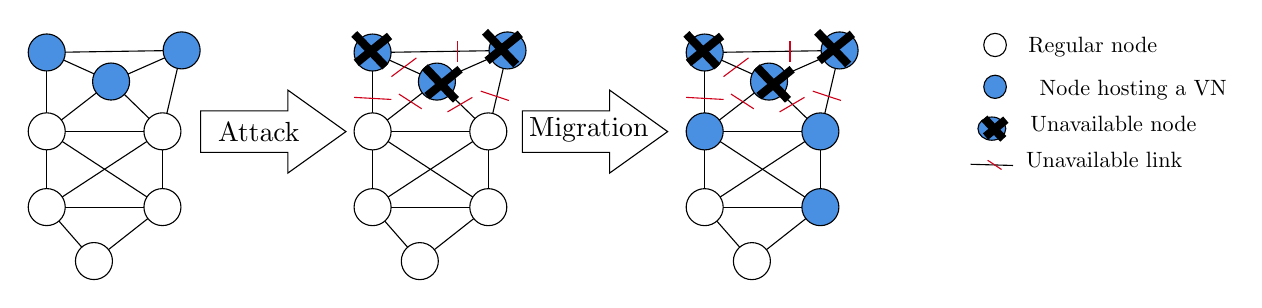
\begin{tikzpicture}[x=0.75pt,y=0.75pt,yscale=-1,xscale=1]
%uncomment if require: \path (0,300); %set diagram left start at 0, and has height of 300

%Shape: Ellipse [id:dp8430130954948494] 
\draw  [fill={rgb, 255:red, 74; green, 144; blue, 226 }  ,fill opacity=1 ] (461.48,51.56) .. controls (461.48,48.47) and (464.48,45.97) .. (468.19,45.97) .. controls (471.9,45.97) and (474.9,48.47) .. (474.9,51.56) .. controls (474.9,54.66) and (471.9,57.16) .. (468.19,57.16) .. controls (464.48,57.16) and (461.48,54.66) .. (461.48,51.56) -- cycle ;
%Shape: Ellipse [id:dp5907962461562573] 
\draw  [fill={rgb, 255:red, 74; green, 144; blue, 226 }  ,fill opacity=1 ] (464.29,31.43) .. controls (464.29,28.34) and (466.73,25.83) .. (469.74,25.83) .. controls (472.75,25.83) and (475.19,28.34) .. (475.19,31.43) .. controls (475.19,34.52) and (472.75,37.02) .. (469.74,37.02) .. controls (466.73,37.02) and (464.29,34.52) .. (464.29,31.43) -- cycle ;
%Straight Lines [id:da1514909222057811] 
\draw [color={rgb, 255:red, 0; green, 0; blue, 0 }  ,draw opacity=1 ]   (458,68.75) -- (478.38,69.32) ;


%Shape: Ellipse [id:dp8047559285598944] 
\draw  [fill={rgb, 255:red, 255; green, 255; blue, 255 }  ,fill opacity=1 ] (464.29,11.26) .. controls (464.29,8.17) and (466.73,5.67) .. (469.74,5.67) .. controls (472.75,5.67) and (475.19,8.17) .. (475.19,11.26) .. controls (475.19,14.35) and (472.75,16.86) .. (469.74,16.86) .. controls (466.73,16.86) and (464.29,14.35) .. (464.29,11.26) -- cycle ;
%Straight Lines [id:da5581047744563914] 
\draw [color={rgb, 255:red, 208; green, 2; blue, 27 }  ,draw opacity=1 ]   (472.87,71.26) -- (466.14,66.8) ;


%Straight Lines [id:da6983464143799673] 
\draw [line width=3]    (464.54,46.62) -- (473.71,56.51) ;


%Straight Lines [id:da20248481970311139] 
\draw [line width=3]    (465.15,55.41) -- (474.93,47.25) ;



%Straight Lines [id:da6176709448343998] 
\draw    (200.83,28.91) -- (225.58,52.91) ;


%Straight Lines [id:da5463688705908274] 
\draw    (200.83,28.91) -- (169.83,52.91) ;


%Straight Lines [id:da11538810799649779] 
\draw    (234.83,13.91) -- (225.92,51.91) ;


%Straight Lines [id:da8853756126147032] 
\draw    (169.83,14.91) -- (169.83,52.91) ;


%Straight Lines [id:da5031310157957251] 
\draw    (169.83,52.91) -- (225.58,89.41) ;


%Straight Lines [id:da8400043886929478] 
\draw    (169.83,89.41) -- (192.58,115.41) ;


%Straight Lines [id:da5242150334882041] 
\draw    (225.58,89.41) -- (192.58,115.41) ;


%Straight Lines [id:da3960630757961663] 
\draw    (225.58,52.91) -- (169.83,89.41) ;


%Shape: Circle [id:dp47175232960651714] 
\draw  [fill={rgb, 255:red, 255; green, 255; blue, 255 }  ,fill opacity=1 ] (160.92,52.91) .. controls (160.92,47.98) and (164.91,43.99) .. (169.83,43.99) .. controls (174.76,43.99) and (178.75,47.98) .. (178.75,52.91) .. controls (178.75,57.83) and (174.76,61.82) .. (169.83,61.82) .. controls (164.91,61.82) and (160.92,57.83) .. (160.92,52.91) -- cycle ;
%Shape: Circle [id:dp5879580381901867] 
\draw  [fill={rgb, 255:red, 255; green, 255; blue, 255 }  ,fill opacity=1 ] (216.67,52.91) .. controls (216.67,47.98) and (220.66,43.99) .. (225.58,43.99) .. controls (230.51,43.99) and (234.5,47.98) .. (234.5,52.91) .. controls (234.5,57.83) and (230.51,61.82) .. (225.58,61.82) .. controls (220.66,61.82) and (216.67,57.83) .. (216.67,52.91) -- cycle ;
%Shape: Circle [id:dp5579759383684684] 
\draw  [fill={rgb, 255:red, 255; green, 255; blue, 255 }  ,fill opacity=1 ] (160.92,89.41) .. controls (160.92,84.48) and (164.91,80.49) .. (169.83,80.49) .. controls (174.76,80.49) and (178.75,84.48) .. (178.75,89.41) .. controls (178.75,94.33) and (174.76,98.32) .. (169.83,98.32) .. controls (164.91,98.32) and (160.92,94.33) .. (160.92,89.41) -- cycle ;
%Shape: Circle [id:dp885869190555082] 
\draw  [fill={rgb, 255:red, 255; green, 255; blue, 255 }  ,fill opacity=1 ] (216.67,89.41) .. controls (216.67,84.48) and (220.66,80.49) .. (225.58,80.49) .. controls (230.51,80.49) and (234.5,84.48) .. (234.5,89.41) .. controls (234.5,94.33) and (230.51,98.32) .. (225.58,98.32) .. controls (220.66,98.32) and (216.67,94.33) .. (216.67,89.41) -- cycle ;
%Shape: Circle [id:dp3254884021888832] 
\draw  [fill={rgb, 255:red, 255; green, 255; blue, 255 }  ,fill opacity=1 ] (183.67,115.41) .. controls (183.67,110.48) and (187.66,106.49) .. (192.58,106.49) .. controls (197.51,106.49) and (201.5,110.48) .. (201.5,115.41) .. controls (201.5,120.33) and (197.51,124.32) .. (192.58,124.32) .. controls (187.66,124.32) and (183.67,120.33) .. (183.67,115.41) -- cycle ;
%Straight Lines [id:da7041582060743201] 
\draw    (178.75,52.91) -- (216.67,52.91) ;


%Straight Lines [id:da26176464493068274] 
\draw    (178.75,89.41) -- (216.67,89.41) ;


%Straight Lines [id:da45312150436944487] 
\draw    (225.58,80.49) -- (225.58,61.82) ;


%Straight Lines [id:da10497643854199257] 
\draw    (169.83,61.82) -- (169.83,80.49) ;


%Straight Lines [id:da023464273570334315] 
\draw    (169.83,14.91) -- (234.83,13.91) ;


%Straight Lines [id:da7461511731963238] 
\draw    (200.83,28.91) -- (234.83,13.91) ;


%Straight Lines [id:da6717008743630867] 
\draw    (169.83,14.91) -- (200.83,28.91) ;


%Shape: Circle [id:dp17672294199894456] 
\draw  [fill={rgb, 255:red, 74; green, 144; blue, 226 }  ,fill opacity=1 ] (160.92,14.91) .. controls (160.92,9.98) and (164.91,5.99) .. (169.83,5.99) .. controls (174.76,5.99) and (178.75,9.98) .. (178.75,14.91) .. controls (178.75,19.83) and (174.76,23.82) .. (169.83,23.82) .. controls (164.91,23.82) and (160.92,19.83) .. (160.92,14.91) -- cycle ;
%Shape: Circle [id:dp8878711028556632] 
\draw  [fill={rgb, 255:red, 74; green, 144; blue, 226 }  ,fill opacity=1 ] (191.92,28.91) .. controls (191.92,23.98) and (195.91,19.99) .. (200.83,19.99) .. controls (205.76,19.99) and (209.75,23.98) .. (209.75,28.91) .. controls (209.75,33.83) and (205.76,37.82) .. (200.83,37.82) .. controls (195.91,37.82) and (191.92,33.83) .. (191.92,28.91) -- cycle ;
%Shape: Circle [id:dp02560438280336974] 
\draw  [fill={rgb, 255:red, 74; green, 144; blue, 226 }  ,fill opacity=1 ] (225.92,13.91) .. controls (225.92,8.98) and (229.91,4.99) .. (234.83,4.99) .. controls (239.76,4.99) and (243.75,8.98) .. (243.75,13.91) .. controls (243.75,18.83) and (239.76,22.82) .. (234.83,22.82) .. controls (229.91,22.82) and (225.92,18.83) .. (225.92,13.91) -- cycle ;
%Straight Lines [id:da7816159630212767] 
\draw [color={rgb, 255:red, 208; green, 2; blue, 27 }  ,draw opacity=1 ]   (210.92,9.51) -- (210.92,19.51) ;


%Straight Lines [id:da23242280473047117] 
\draw [color={rgb, 255:red, 208; green, 2; blue, 27 }  ,draw opacity=1 ]   (221.92,33.51) -- (235.5,38.01) ;


%Straight Lines [id:da25217250177313655] 
\draw [color={rgb, 255:red, 208; green, 2; blue, 27 }  ,draw opacity=1 ]   (160.92,36.51) -- (178.92,37.51) ;


%Straight Lines [id:da8252457737222165] 
\draw [color={rgb, 255:red, 208; green, 2; blue, 27 }  ,draw opacity=1 ]   (178.92,26.51) -- (190.92,17.51) ;


%Straight Lines [id:da6307655523636441] 
\draw [color={rgb, 255:red, 208; green, 2; blue, 27 }  ,draw opacity=1 ]   (205.92,43.51) -- (217.92,36.51) ;


%Straight Lines [id:da5703265914230616] 
\draw [color={rgb, 255:red, 208; green, 2; blue, 27 }  ,draw opacity=1 ]   (193.5,42.01) -- (182.5,34.91) ;


%Straight Lines [id:da3989594608358942] 
\draw [line width=3]    (161,5.93) -- (176,21.68) ;


%Straight Lines [id:da7318288975856456] 
\draw [line width=3]    (162,19.93) -- (178,6.93) ;



%Straight Lines [id:da9963706937012238] 
\draw [line width=3]    (224,4.93) -- (239,20.68) ;


%Straight Lines [id:da43798340024618054] 
\draw [line width=3]    (225,18.93) -- (241,5.93) ;



%Straight Lines [id:da5033136183613764] 
\draw [line width=3]    (195,21.93) -- (210,37.68) ;


%Straight Lines [id:da623542865534238] 
\draw [line width=3]    (196,35.93) -- (212,22.93) ;




%Straight Lines [id:da021425369536150374] 
\draw    (43.83,28.87) -- (68.58,52.87) ;


%Straight Lines [id:da809644771756096] 
\draw    (43.83,28.87) -- (12.83,52.87) ;


%Straight Lines [id:da9075994171710501] 
\draw    (77.83,13.87) -- (68.92,51.87) ;


%Straight Lines [id:da7475460187374237] 
\draw    (12.83,14.87) -- (12.83,52.87) ;


%Straight Lines [id:da06975692875380135] 
\draw    (12.83,52.87) -- (68.58,89.37) ;


%Straight Lines [id:da9394544948671463] 
\draw    (12.83,89.37) -- (35.58,115.37) ;


%Straight Lines [id:da46361116523850066] 
\draw    (68.58,89.37) -- (35.58,115.37) ;


%Straight Lines [id:da9816638193583865] 
\draw    (68.58,52.87) -- (12.83,89.37) ;


%Shape: Circle [id:dp21531756732058427] 
\draw  [fill={rgb, 255:red, 255; green, 255; blue, 255 }  ,fill opacity=1 ] (3.92,52.87) .. controls (3.92,47.95) and (7.91,43.96) .. (12.83,43.96) .. controls (17.76,43.96) and (21.75,47.95) .. (21.75,52.87) .. controls (21.75,57.8) and (17.76,61.79) .. (12.83,61.79) .. controls (7.91,61.79) and (3.92,57.8) .. (3.92,52.87) -- cycle ;
%Shape: Circle [id:dp32258921480580105] 
\draw  [fill={rgb, 255:red, 255; green, 255; blue, 255 }  ,fill opacity=1 ] (59.67,52.87) .. controls (59.67,47.95) and (63.66,43.96) .. (68.58,43.96) .. controls (73.51,43.96) and (77.5,47.95) .. (77.5,52.87) .. controls (77.5,57.8) and (73.51,61.79) .. (68.58,61.79) .. controls (63.66,61.79) and (59.67,57.8) .. (59.67,52.87) -- cycle ;
%Shape: Circle [id:dp7783815840311967] 
\draw  [fill={rgb, 255:red, 255; green, 255; blue, 255 }  ,fill opacity=1 ] (3.92,89.37) .. controls (3.92,84.45) and (7.91,80.46) .. (12.83,80.46) .. controls (17.76,80.46) and (21.75,84.45) .. (21.75,89.37) .. controls (21.75,94.3) and (17.76,98.29) .. (12.83,98.29) .. controls (7.91,98.29) and (3.92,94.3) .. (3.92,89.37) -- cycle ;
%Shape: Circle [id:dp9106798970146953] 
\draw  [fill={rgb, 255:red, 255; green, 255; blue, 255 }  ,fill opacity=1 ] (59.67,89.37) .. controls (59.67,84.45) and (63.66,80.46) .. (68.58,80.46) .. controls (73.51,80.46) and (77.5,84.45) .. (77.5,89.37) .. controls (77.5,94.3) and (73.51,98.29) .. (68.58,98.29) .. controls (63.66,98.29) and (59.67,94.3) .. (59.67,89.37) -- cycle ;
%Shape: Circle [id:dp1831427544072476] 
\draw  [fill={rgb, 255:red, 255; green, 255; blue, 255 }  ,fill opacity=1 ] (26.67,115.37) .. controls (26.67,110.45) and (30.66,106.46) .. (35.58,106.46) .. controls (40.51,106.46) and (44.5,110.45) .. (44.5,115.37) .. controls (44.5,120.3) and (40.51,124.29) .. (35.58,124.29) .. controls (30.66,124.29) and (26.67,120.3) .. (26.67,115.37) -- cycle ;
%Straight Lines [id:da9700158448121917] 
\draw    (21.75,52.87) -- (59.67,52.87) ;


%Straight Lines [id:da010185511635833033] 
\draw    (21.75,89.37) -- (59.67,89.37) ;


%Straight Lines [id:da4677014236726348] 
\draw    (68.58,80.46) -- (68.58,61.79) ;


%Straight Lines [id:da19862578341507608] 
\draw    (12.83,61.79) -- (12.83,80.46) ;


%Straight Lines [id:da6877311034443738] 
\draw    (12.83,14.87) -- (77.83,13.87) ;


%Straight Lines [id:da39601253001890035] 
\draw    (43.83,28.87) -- (77.83,13.87) ;


%Straight Lines [id:da8270994037474519] 
\draw    (12.83,14.87) -- (43.83,28.87) ;


%Shape: Circle [id:dp2984826737185816] 
\draw  [fill={rgb, 255:red, 74; green, 144; blue, 226 }  ,fill opacity=1 ] (3.92,14.87) .. controls (3.92,9.95) and (7.91,5.96) .. (12.83,5.96) .. controls (17.76,5.96) and (21.75,9.95) .. (21.75,14.87) .. controls (21.75,19.8) and (17.76,23.79) .. (12.83,23.79) .. controls (7.91,23.79) and (3.92,19.8) .. (3.92,14.87) -- cycle ;
%Shape: Circle [id:dp6437572475375565] 
\draw  [fill={rgb, 255:red, 74; green, 144; blue, 226 }  ,fill opacity=1 ] (34.92,28.87) .. controls (34.92,23.95) and (38.91,19.96) .. (43.83,19.96) .. controls (48.76,19.96) and (52.75,23.95) .. (52.75,28.87) .. controls (52.75,33.8) and (48.76,37.79) .. (43.83,37.79) .. controls (38.91,37.79) and (34.92,33.8) .. (34.92,28.87) -- cycle ;
%Shape: Circle [id:dp23183818676236623] 
\draw  [fill={rgb, 255:red, 74; green, 144; blue, 226 }  ,fill opacity=1 ] (68.92,13.87) .. controls (68.92,8.95) and (72.91,4.96) .. (77.83,4.96) .. controls (82.76,4.96) and (86.75,8.95) .. (86.75,13.87) .. controls (86.75,18.8) and (82.76,22.79) .. (77.83,22.79) .. controls (72.91,22.79) and (68.92,18.8) .. (68.92,13.87) -- cycle ;

%Right Arrow [id:dp417684980473099] 
\draw   (87,43) -- (129,43) -- (129,33) -- (157,53) -- (129,73) -- (129,63) -- (87,63) -- cycle ;

%Right Arrow [id:dp6623970589974628] 
\draw   (242,43) -- (284,43) -- (284,33) -- (312,53) -- (284,73) -- (284,63) -- (242,63) -- cycle ;
%Straight Lines [id:da22163993557127015] 
\draw    (360.83,28.91) -- (385.58,52.91) ;


%Straight Lines [id:da8341652491193966] 
\draw    (360.83,28.91) -- (329.83,52.91) ;


%Straight Lines [id:da14662408338887967] 
\draw    (394.83,13.91) -- (385.92,51.91) ;


%Straight Lines [id:da1054361182628697] 
\draw    (329.83,14.91) -- (329.83,52.91) ;


%Straight Lines [id:da878058282787745] 
\draw    (329.83,52.91) -- (385.58,89.41) ;


%Straight Lines [id:da5143639640863213] 
\draw    (329.83,89.41) -- (352.58,115.41) ;


%Straight Lines [id:da38106162801473] 
\draw    (385.58,89.41) -- (352.58,115.41) ;


%Straight Lines [id:da9515281954413589] 
\draw    (385.58,52.91) -- (329.83,89.41) ;


%Shape: Circle [id:dp7012949201072771] 
\draw  [fill={rgb, 255:red, 74; green, 144; blue, 226 }  ,fill opacity=1 ] (320.92,52.91) .. controls (320.92,47.98) and (324.91,43.99) .. (329.83,43.99) .. controls (334.76,43.99) and (338.75,47.98) .. (338.75,52.91) .. controls (338.75,57.83) and (334.76,61.82) .. (329.83,61.82) .. controls (324.91,61.82) and (320.92,57.83) .. (320.92,52.91) -- cycle ;
%Shape: Circle [id:dp8511635916765001] 
\draw  [fill={rgb, 255:red, 74; green, 144; blue, 226 }  ,fill opacity=1 ] (376.67,52.91) .. controls (376.67,47.98) and (380.66,43.99) .. (385.58,43.99) .. controls (390.51,43.99) and (394.5,47.98) .. (394.5,52.91) .. controls (394.5,57.83) and (390.51,61.82) .. (385.58,61.82) .. controls (380.66,61.82) and (376.67,57.83) .. (376.67,52.91) -- cycle ;
%Shape: Circle [id:dp10253503783482376] 
\draw  [fill={rgb, 255:red, 255; green, 255; blue, 255 }  ,fill opacity=1 ] (320.92,89.41) .. controls (320.92,84.48) and (324.91,80.49) .. (329.83,80.49) .. controls (334.76,80.49) and (338.75,84.48) .. (338.75,89.41) .. controls (338.75,94.33) and (334.76,98.32) .. (329.83,98.32) .. controls (324.91,98.32) and (320.92,94.33) .. (320.92,89.41) -- cycle ;
%Shape: Circle [id:dp7321236156986349] 
\draw  [fill={rgb, 255:red, 74; green, 144; blue, 226 }  ,fill opacity=1 ] (376.67,89.41) .. controls (376.67,84.48) and (380.66,80.49) .. (385.58,80.49) .. controls (390.51,80.49) and (394.5,84.48) .. (394.5,89.41) .. controls (394.5,94.33) and (390.51,98.32) .. (385.58,98.32) .. controls (380.66,98.32) and (376.67,94.33) .. (376.67,89.41) -- cycle ;
%Shape: Circle [id:dp8317705860942972] 
\draw  [fill={rgb, 255:red, 255; green, 255; blue, 255 }  ,fill opacity=1 ] (343.67,115.41) .. controls (343.67,110.48) and (347.66,106.49) .. (352.58,106.49) .. controls (357.51,106.49) and (361.5,110.48) .. (361.5,115.41) .. controls (361.5,120.33) and (357.51,124.32) .. (352.58,124.32) .. controls (347.66,124.32) and (343.67,120.33) .. (343.67,115.41) -- cycle ;
%Straight Lines [id:da11492821108610518] 
\draw    (338.75,52.91) -- (376.67,52.91) ;


%Straight Lines [id:da6428199077173957] 
\draw    (338.75,89.41) -- (376.67,89.41) ;


%Straight Lines [id:da4443653918115038] 
\draw    (385.58,80.49) -- (385.58,61.82) ;


%Straight Lines [id:da5181998888947625] 
\draw    (329.83,61.82) -- (329.83,80.49) ;


%Straight Lines [id:da8991729748789462] 
\draw    (329.83,14.91) -- (394.83,13.91) ;


%Straight Lines [id:da6133921287796495] 
\draw    (360.83,28.91) -- (394.83,13.91) ;


%Straight Lines [id:da3198353622868253] 
\draw    (329.83,14.91) -- (360.83,28.91) ;


%Shape: Circle [id:dp32555515723538997] 
\draw  [fill={rgb, 255:red, 74; green, 144; blue, 226 }  ,fill opacity=1 ] (320.92,14.91) .. controls (320.92,9.98) and (324.91,5.99) .. (329.83,5.99) .. controls (334.76,5.99) and (338.75,9.98) .. (338.75,14.91) .. controls (338.75,19.83) and (334.76,23.82) .. (329.83,23.82) .. controls (324.91,23.82) and (320.92,19.83) .. (320.92,14.91) -- cycle ;
%Shape: Circle [id:dp479820223624436] 
\draw  [fill={rgb, 255:red, 74; green, 144; blue, 226 }  ,fill opacity=1 ] (351.92,28.91) .. controls (351.92,23.98) and (355.91,19.99) .. (360.83,19.99) .. controls (365.76,19.99) and (369.75,23.98) .. (369.75,28.91) .. controls (369.75,33.83) and (365.76,37.82) .. (360.83,37.82) .. controls (355.91,37.82) and (351.92,33.83) .. (351.92,28.91) -- cycle ;
%Shape: Circle [id:dp49048798397317805] 
\draw  [fill={rgb, 255:red, 74; green, 144; blue, 226 }  ,fill opacity=1 ] (385.92,13.91) .. controls (385.92,8.98) and (389.91,4.99) .. (394.83,4.99) .. controls (399.76,4.99) and (403.75,8.98) .. (403.75,13.91) .. controls (403.75,18.83) and (399.76,22.82) .. (394.83,22.82) .. controls (389.91,22.82) and (385.92,18.83) .. (385.92,13.91) -- cycle ;
%Straight Lines [id:da2877242408536883] 
\draw [color={rgb, 255:red, 208; green, 2; blue, 27 }  ,draw opacity=1 ]   (370.92,9.51) -- (370.92,19.51) ;


%Straight Lines [id:da384891491483089] 
\draw [color={rgb, 255:red, 208; green, 2; blue, 27 }  ,draw opacity=1 ]   (381.92,33.51) -- (395.5,38.01) ;


%Straight Lines [id:da9676951250293255] 
\draw [color={rgb, 255:red, 208; green, 2; blue, 27 }  ,draw opacity=1 ]   (320.92,36.51) -- (338.92,37.51) ;


%Straight Lines [id:da8030081016605746] 
\draw [color={rgb, 255:red, 208; green, 2; blue, 27 }  ,draw opacity=1 ]   (338.92,26.51) -- (350.92,17.51) ;


%Straight Lines [id:da14577170595095879] 
\draw [color={rgb, 255:red, 208; green, 2; blue, 27 }  ,draw opacity=1 ]   (365.92,43.51) -- (377.92,36.51) ;


%Straight Lines [id:da1498283509390178] 
\draw [color={rgb, 255:red, 208; green, 2; blue, 27 }  ,draw opacity=1 ]   (353.5,42.01) -- (342.5,34.91) ;


%Straight Lines [id:da7540175814554593] 
\draw [line width=3]    (321,5.93) -- (336,21.68) ;


%Straight Lines [id:da08956624030773497] 
\draw [line width=3]    (322,19.93) -- (338,6.93) ;



%Straight Lines [id:da4115477309546427] 
\draw [line width=3]    (384,4.93) -- (399,20.68) ;


%Straight Lines [id:da6038706591283135] 
\draw [line width=3]    (385,18.93) -- (401,5.93) ;



%Straight Lines [id:da5077658828074341] 
\draw [line width=3]    (355,21.93) -- (370,37.68) ;


%Straight Lines [id:da9268834839804526] 
\draw [line width=3]    (356,35.93) -- (372,22.93) ;




% Text Node
\draw (516.81,12.09) node [scale=0.8] [align=left] {Regular node};
% Text Node
\draw (536.31,33.08) node [scale=0.8] [align=left] {Node hosting a VN};
% Text Node
\draw (526.81,49.09) node [scale=0.8] [align=left] {Unavailable node};
% Text Node
\draw (522.31,66.56) node [scale=0.8] [align=left] {Unavailable link};
% Text Node
\draw (274,52) node  [align=left] {Migration};
% Text Node
\draw (115,53) node  [align=left] {Attack};


\end{tikzpicture}



\caption{Migration triggered by the attacker}
\label{fig:trigger}

\end{figure*}

\subsubsection{Attacker Model}
\label{sec:attack_model}

Fig.~\ref{fig:trigger} depicts the evolution of the infrastructure after the attacker has rendered part of it unavailable. 
At first, the virtual network is running on a healthy physical substrate; but once the attack is launched, the substrate becomes unavailable and the virtual network must be migrated quickly to reduce the end user's service interruption.

\paragraph{Objectives}
Figure~\ref{fig:data-exfiltration-attack} illustrates the attacker's objective.
In order to exfiltrate the network traffic of his victim, the attacker will compromise nodes in the infrastructure. The nodes he will attack will be used to create a path between the victim's network and an exfiltration point (\eg a Virtual Machine) owned by the attacker.

We make several hypotheses regarding the capacities and resources of an attacker:
\paragraph{Hypotheses}
\begin{itemize}
    \item The attacker can modify the configuration of network nodes.
    
    Modifying a node's configuration has been proven  possible in~\cite{Taxonomy_Hizver2015, Bokani2015, attain-Ujcich2017}.Precisely, the attacker is able to spoof the identity of the network hypervisor, and thus is able to inject malicious flow rules inside the nodes to create the data exfiltration path. 
    However, he is not able to be designated as the original network hypervisor in the nodes' configurations. 
    This can be explained because it requires advanced configuration privileges. Moreover, a physical node missing from the legitimate hypervisor's topology view is easily detectable, in comparison to malicious flow rules injected inside the physical nodes.
    
    \item The attacker is able to exfiltrate data from his victim's VN.
    
    The exfiltration of data from the network only requires a Virtual Machine to forward the traffic to.
    
    \item The attacker only targets one VN during the attack.
    
     The attacker has performed enough information gathering to determine which VN is the most profitable to attack.
     
    
    \item The attacker can collect information to determine which nodes to target.
    
    The attacker has been able to determine which nodes to attack to trigger the migration thanks to prior scanning and information gathering. 
    Nevertheless, he has no exact knowledge about which nodes will be selected as the destination substrate and he will discover it by doing further scanning and fingerprinting  while he is attacking the infrastructure.  
    We can find a description of such techniques in~\cite{Hong2015,Sphinx-Dhawan2015}.
    This information gathering is out of scope of this thesis.
    
    \item The attacker owns several VMs in the infrastructure.
    
     Owning several VMs in the infrastructure only incurs a small financial cost in any existing virtualization environment.
 
    
    \item There may be several attack sources in the infrastructure.
    
    The attacker owns several VMs in the infrastructure and may leverage vulnerabilities in multiple locations.
    
    \item A node will always be attacked by the same source.
    
    Because of the short time interval considered for the migration, we suppose that the attack will always take the same path (\ie no change in the flow rules for routing the attack).
    Additionally, the attacker defines at the beginning the source of each attack for each node and does not deviate from this afterwards.
    Th path of the attack will be considered to determine the global detection probability of the attack.
    
    \item The attacker only attacks one node at a time.
    
    We make this assumption for the consistency with the assumption that the migration process itself is sequential~\cite{Lime-Ghorbani2014}.
    
    
    \item An attacker needs a certain amount of time to complete his attack.
    
    Because the attacker targets one node at a time, it will take several steps to completely establish the full path to exfiltrate data. 
    
    \item The attacker only targets nodes contributing to construct the exfiltration path.
    
     Even if the attacker may target all nodes in the infrastructure, he has no incentives to attack nodes that will not be part of the path to exfiltrate data from his victim's network. We consider that the attacker will choose his targets using the strategy from Section~\ref{sec:target_proba}.
    From the point of view of the defender, it is impossible to accurately know which node will be attacked.
    
\end{itemize}




% , since all the nodes monitoring the path may see the attack come through.
% \GB{so this is very important to understand at what level is located the attacker. Is she another tenant? Or does she have access to the substrate? Do attack packets flow at the data plane or at the control plane?}.\FC{The attack is routed in the control plane but impacts the data plane. I don't want to go to deep in details so we do not add too much confusion. We can simplify by saying that the control plane topology is the same as the data plane topology.}

\subsubsection{Assumptions}
\label{sec:mdp-system-hypotheses}
We describe here the assumptions made about the infrastructure and the migration process.

% \textbf{Migration}
\begin{itemize}
    \item
    The migration will deploy in the target physical substrate all the flow rules necessary to operate the Virtual Network properly. In this chapter the expression ``migrating a node" means deploying configuration rules in a physical node.
    
    \item
    We consider that the migration of the virtual nodes is sequential~\cite{Lime-Ghorbani2014}, thus the nodes will be migrated one at a time.
    We suppose that both Virtual Network and physical infrastructure are static (\ie the topology does not change over time).
    
    \item All nodes in the original substrate have been fully compromised by the attacker and thus are not considered as candidates for the destination substrate.  
    This assumption is reinforced by the fact that forcing all the resources to be reallocated could be leveraged by the attacker in an attempt to have the target Virtual Network relocated closer to his Virtual Machines.
    Virtual Machines are already subject to such attacks, as presented by Atya \etal in~\cite{stalling-atya2017,malicious-atya2017}.

    \item
    We also assume that migration time is uniform across all nodes (\ie no node takes longer to migrate in the infrastructure than another).
    
    \item
     We consider the Virtual Network equivalent to the physical nodes composing its embedding.
     This assumption is used to represent how nodes will be migrated and on which node flow rules will be installed. 
\end{itemize}



\subsubsection{Modeling the RA problem with a MDP}
\label{sec:mdp-model}
In this section, we describe our MDP addressing the problem of optimal defense resource allocation for Virtual Network migration.

\subsubsection{Model assumptions}
\label{sec:mdp-model-assumption}

\textbf{Monitoring}
\begin{itemize}
    \item The deployment of the monitoring on the nodes impacts the infrastructure's performance. 
    
    \item The infrastructure owner is willing to bear a limited impact on the performance.
    % Based on the work of Ismail \etal~\cite{interdep-ismail2017}, we consider the monitoring cost  proportional to the intrinsic value of the nodes (\eg CPU time on a powerful machine is more expensive compared to a smaller one).
    
    \item We consider the monitoring imperfect with a certain attack detection probability.
    Each node on the path of an attack has the same probability to detect it, \ie there is no node more efficient than another. 
\end{itemize}


\textbf{Targeting nodes}
% \label{sec:attacking}
% \GB{one of the main assumptions is therefore that the attack path is in the substrate}
% \FC{The attack path is from attacker to target node. However, the other path, the path used to exfiltrate data will be in the substrate obviously. I will differentiate these two types of paths}
\begin{itemize}
    \item  Physical nodes embedding the VN are more likely to be attacked than other nodes used to construct the exfiltration path.
    
    During the migration, the attacker will target nodes to construct the path to exfiltrate data from the victim's VN.
    Embedding nodes are more important since at least one embedding node must be part of the path leading to the exfiltration point.
    
    \item The attacker's strategy for choosing which nodes he attacks is based on the information gathering he performs while attacking. 
    
    The details of such activity is considered out of the scope of this thesis.
    Similar work on cloud environments for virtual machines colocation has been proposed in~\cite{getoffmucloud-Ristenpart2009, incentivemtd-Zhang2012}.
    Johnson \etal propose in~\cite{mitigateAPT-johnson2013} a real time metric that determines the node that is the most likely to be the next target of an attack.
    
    \item
    If the attacker was able to establish the full path then we consider that the global attack was successful.
    
    A full path between the attacker and his victim's is connecting at least one physical node embedding the victim's VN to a virtual machine owned by the attacker. Such path is illustrated in Figure~\ref{fig:data-exfiltration-attack}.
\end{itemize}



\subsubsection{States}
\label{sec:stateset}
The states in the MDP represent the evolution of the infrastructure, \ie the progress of the migration, the remaining resources as well as the compromised nodes in the infrastructure.
The defender has two different resources: $b_f$, the global amount of time the migration is going to take, and $b_c$ the global computational power available for the monitoring.
Precisely, $b_c$ corresponds to the overall performance impact caused by the monitoring. % the defender is willing to perform.
%  on the network virtualization service
This represents the amount of resources that can be spent to perform monitoring instead of operational tasks.

% \GB{is $b_c = 0$ a halt condition?}\FC{No, monitoring actions are just not available, and choosing them only cost budget with no reward}.

%GB redundancy detected, so I commented out the following lines
We describe the state of the system as the following tuple: $s=<b_f,b_c,Mi,Mo,At>$:
\begin{itemize}
    \item $n$: The number of nodes in the infrastructure.
    \item $\textbf{N} = \{1,..,n\}$ is the set of nodes in the infrastructure.
    \item $Mi^s \subset \textbf{N} $ is the set of currently migrated nodes for state $s\in S$.
    \item $Mo^s \subset \textbf{N}$ is the set of currently monitored nodes for state $s\in S$.
    \item $At^s \subset \textbf{N}$ is the set of compromised nodes for state $s \in S$.
    \item $b_f^s$ is the time left before the end of the migration at state $s$.
    \item $b_c^s$ is the remaining computational power at state $s$.
\end{itemize}

% We remind the reader that an absorbing state is a state where all actions transition back to itself.

\subsubsection{Actions}
\label{sec:actionset}
The defender can either add monitoring on a particular node in the infrastructure, remove this monitoring, or choose to do nothing.
The option of doing nothing prevents counter-productive options like forcing undesired actions (\eg removing monitoring from a node that is not currently monitoring the infrastructure).
We note $m_j$ the action of setting up monitoring on node $j$. Similarly, we note $u_j$ the action of removing monitoring on node $j$.
Finally we note $d$ the action of doing nothing.
%\\With $n$ being the number of nodes in the infrastructure 
\\We define $A = \{m_1,..,m_n,u_1,..,u_n,d\}$ as the set of actions available at each state.
% \GB{you really need to defined this term. What does it involve?}
% \FC{What do you think about that ?}

% \FC{The last node added to the path should be the node belonging to $\mathbb{Z}$ because otherwise exfiltrating data without the full path will raise a lot of unexpected $packet-in$ . This may not be an issue though}
% We also assume he may construct the full path by connecting nodes one after another instead of randomly constructing the chain. 

\subsubsection{Cost of actions}
Choosing an action impacts both $b_f$ and $b_c$ resources. The action will make the migration progress by one step.
We note $c_f$ the time it takes to migrate one node, and based on the assumption made in Section~\ref{sec:mdp-system-hypotheses}, we define it as equal for each action.

Each node $j \in \textbf{N}$ is characterized by an intrinsic value $V_j \in \mathbb{R}$ that can be seen as the financial value of the node.
% , its computing capacities and its function inside the virtualization infrastructure. 
%We note $\{V_1,..,V_n\}, \forall i~V_i \in \mathbb{R}$ as the set of said values, one for each node. 
Based on the work of Ismail~\etal~\cite{interdep-ismail2017}, we consider that the cost of deploying monitoring on each node is not uniform and depends on its intrinsic value. We represent this by assigning a proportionality coefficient to each node.
We note this coefficient $k^j_{c}$, associated to $b_c$ and node $j$.
Then we define the monitoring cost $c_c^j$ for node $j$ as : $\forall j \in \textbf{N},~ c_c^j = k^j_{c}  V_j$

We summarize $c_f$ and $c_c^j$ with:

\begin{equation}
  \begin{cases}
    c_f\text{ is a constant}\\
   \forall j \in \textbf{N},~ c_c^j = k^j_{c}  V_j 
  \end{cases}
\end{equation}

\subsubsection{Probabilistic target determination}
\label{sec:target_proba}
We consider the path taken by the attack as a set of nodes.
% We name $L$ the set of paths inside the infrastructure. 
We define $L_j$ the unique path leading the attacker to node $j$.
We note $\textbf{W}$ the set of non compromised nodes that are currently hosting the migrated Virtual Network (\ie $\textbf{W} = Mi^s \cap \overline{At^s})$.
Similarly, we note $\textbf{T}$ the set of non compromised nodes that are directly connected to a compromised node and are not part of $\textbf{W}$, \ie they are potential candidates for the path between attacker and victim. Alg.~\ref{algo:target} is computed at each state as the sets $\textbf{T}$ and $\textbf{W}$ are changing.
% This implies that compromising a node in $\mathbb{T}$
% \FC{Add algorithm for function q to determine targets}
\begin{algorithm}
 \SetKwInOut{Input}{Input}
 \SetKwInOut{Output}{Output}
 \Input{\textbf{W}, \textbf{T}, current state $s$, \textit{n} nodes}
 \Output{\textit{n} probabilities to attack each of \textit{n} nodes}
 initialization\;
 \ForEach{node $j$ in \{$1,..,n$\}}{
 \tcc{Is the node part of the embedding  and not compromised ?}
  \uIf{$j \in $\textbf{W} and $Mi^s \cap At^s = \emptyset$}{
   $q(j) = \alpha  \frac{\beta}{\beta|\textbf{W}| + |\textbf{T}|}$
   }
  \tcc{Is the node part of the path to exfiltrate data ?}
  \uElseIf{$j \in $\textbf{T}} {
   $q(j) = \alpha  \frac{1}{\beta|\textbf{W}| + |\textbf{T}|}$
  }
  \Else{
  $q(j)=0$
  }
 }
 \caption{Probabilistic target determination}
 \label{algo:target}
\end{algorithm}


We note $q(j)$ the probability of node $j$ to be attacked as the combination of the probability for an attack to be launched (\ie $\alpha$) and the probability of node $j$ to be chosen among all the nodes in $\textbf{T}$ and $\textbf{W}$ (lines 4 and 6). We also use a coefficient $\beta$ to give more weight to the nodes in $\textbf{W}$, referring to the assumption made in~\ref{sec:mdp-model-assumption}.
Once a substrate node has been compromised, the attacker will finalize the exfiltration set-up by completing the path between his VM and the victim's network.


\subsubsection{Transitions}
We describe the coherence of the MDP states with the following transition constraints:

\begin{enumerate}
    \item If there is no time left (\ie the resource $b_f$ is depleted), a state cannot transition to another state (absorbing state)
    \label{cond:c1}
    \item Choosing an action without the required budget $b_c$ will only cost time (resource $b_f$) with no reward
    \label{cond:c2}
    \item As long as there are nodes to be migrated, each transition will include the migration of one node.
    \label{cond:c3}
    \item A state can only transition to states that preserve the coherence of parameters (resources, etc.)
    \label{cond:c4}
    \item If there is an action too expensive for $b_f$ it will consume the remaining $b_f$ without any reward
    \label{cond:c5}
    \item Choosing an action twice (\ie monitoring a node already monitored) only consumes time ($b_f$) with no reward
    \label{cond:c6}
 \end{enumerate}


When in state $s$ and after choosing an action $a \in A$, the system can transition to $|\textbf{W}|+|\textbf{T}| + 1 $ states, whether an attack happened on one of the nodes or no attack was launched.
We define $S' \subset S$ the set of states to which the state $s$ can transition to with a non null probability.
% We note $s'_{a,j} \in S'$ the state depending on which action $a$ has been chosen and which node will be attacked (index $j$), and if no attack was launched we note $s'_a \in S'$. To ease the reading we simplify $s'_{a,j}$ and $s'_a$ to $s'$ for the rest of this paper.
We define the state modifications once action $a \in A$ has been chosen.
% \GB{I assume $S' \in S$, amirite?}.
% We define $s'_{j} \in S'$ as the state where node $j$ has been attacked and $s'_0$ as the state where no attack happened.
% \GB{what about these below impact computations? how come a state equals a substraction of a cost from another state...}
% \FC{I rewrote the definition of an attribute $s.b_c$ is the $b_c$ budget related to s, see section~\ref{sec:stateset}}
\\
\subparagraph*{\textbf{State modifications for action $m_i$}}
When choosing action $m_i$ at state $s$, we compute the resources impact and set changes for every possible state $s'$. One time step is deducted from $b_f$, the cost of monitoring node $i$ is deducted from $b_c$. Node $i$ is added to the set of monitoring nodes $Mo$ and finally, in case of an attack on node $j$, this node is added to the set of compromised nodes $At$.

\begin{equation}
  s \longrightarrow s' =\begin{cases}
    b_f^{s'} = b_f^s - c_f\\
    b_c^{s'} = b_c^s - c_c^i\\
    Mo^{s'} = Mo^s \cup \{i\}\\
    At^{s'} = At^s \cup \{j\} \text{~~if there is an attack}
  \end{cases}
\end{equation}

\subparagraph*{\textbf{State modifications for action $u_i$}}
When choosing action $u_i$ at state $s$, we compute the resources impact and set changes for every possible state $s'$. One time step is deducted from $b_f$, monitoring node $i$ frees $c_c^i$ and is returned to resource $b_c$. Node $i$ is removed from the set of monitoring nodes $Mo$ and finally, in case of an attack on node $j$, this node is added to the set of compromised nodes $At$.

\begin{equation}
  s \longrightarrow s' =\begin{cases}
    b_f^{s'} = b_f^s - c_f\\
    b_c^{s'} = b_c^s + c_c^i\\
    Mo^{s'} = Mo^s \backslash\{i\}\\
    At^{s'} = At^s \cup \{j\}\text{~~if there is an attack}
  \end{cases}
\end{equation}
% \FC{$ Mo(s) \backslash \{n\}$ means removing n from Mo(s)}

\subparagraph*{\textbf{State modifications for action $d$}}
When choosing action $d$ at state $s$, we compute the resources impact and set changes for every possible state $s'$. One time step is deducted from $b_f$ and in case of an attack on node $j$, this node is added to the set of compromised nodes $At$.
\begin{equation}
  s \longrightarrow s' =\begin{cases}
    b_f^{s'} = b_f^s - c_f\\
    At^{s'} = At^s \cup \{j\}\text{~~if there is an attack}
  \end{cases}
\end{equation}


% We note $\alpha$ the probability of an attack occurring, $q(j)$ the probability of node $j$ being the target of the attack.
% We have defined $q(j)$ with Algorithm~\ref{algo:target}.
We define the transition probability with $\alpha$ and $q(j)$ presented in Section~\ref{sec:target_proba}.
% When in state $s$, the system can transition to N+1 different states, whether an attack had not happened or, which one of the N nodes has been attacked.
% We define $S', s' \in S'$ the set of states to which the state $s$ can transition to.
% We define $s'_{j}$ as the state where node $j$ has been attacked and $s'_0$ as the state where no attack happened.

% Therefore, $s$ will transition with probability $1-\alpha$ when there is no attack or will transition with probability $q(j)$ when attacking node j:

% \begin{itemize}
%     \item $\forall a \in A, P(s,s',a)=1-\alpha$ 
%     \\when there is no attack
    
%     \item $\forall j \in \textbf{N}, \forall a \in A$ , $P(s,s',a)= q(j)$ 
%     \\when attacking node $j$.
% \end{itemize}
\begin{equation}
    P(s,a,s') = \begin{cases}
        1-\alpha \text{ if there is no attack}\\
        q(j)\text{ if node $j$ is attacked, cf. Algorithm~\ref{algo:target}}
    \end{cases}
\end{equation}
\subsubsection{Rewards}

The value of the reward for transitioning takes into account three criteria: the intrinsic value of the nodes, the overall progress of the attacker, and the probability of detecting an attack. The probability of an attack occurring is already accounted for in the transitions.
% The reward represents is impacted whether there was an attack, and if it has been detected.
% In addition to that, an attack only targets one node.
% In the previous sections, we have made assumptions on the path that will be used to attack a node.
% \FC{See suggestions}
If no attack was launched, the reward is based on the value of all the nodes in the infrastructure. 
If an attack was launched, there are two cases: whether the attacker has reached his ultimate goal or not.
If he has, we deduct the value of all the compromised nodes. If he has not, we only deduce the value of the attacked node.
This differentiation comes from the fact that the attacker truly benefits from his attack once the full exfiltration path is established. Before that, the threat is focused on the next node to attack.
% \GB{please use equation environments and refrain from using inline equations.}
%  note $(1-p)^{|L_j \cap Mo|}$ the probability of zero nodes detecting the attack on node j. 
\\We note $\Pi(j)=1 - (1-p)^{|L_j \cap Mo|}$ as the probability of detecting the attack on node $j$ by at least one node. $|L_j \cap Mo|$ represents the number of nodes currently monitoring the infrastructure that will be on the path of the attack, thus the probability for every node not to detect the attack on node $j$ is $(1-p)^{|L_j \cap Mo|}$.
\\
Therefore, we define the following reward function: %, with $s' \in S'$ as in Section~\ref{sec:actionset} :
\\
\begin{equation}
  R(s,a,s') =\begin{cases}
    \sum\limits_{i\in \textbf{N}} V_i \text{, if no attack}\\
    \sum\limits_{i\in \textbf{N}}^n V_i - \sum\limits_{k \in At^s} \overline{\Pi(k)}V_k \text{, if finalized attack }\\
    \sum\limits_{i\in \textbf{N}} V_i - \overline{\Pi(j)}V_j \text{, if partial attack on node $j$}\\
  \end{cases}
\end{equation}

The definition of $R(s,a,s')$ includes the impact of action $a$ in the probability of detecting an attack, as $\Pi(j)$ depends on the monitoring set $Mo$ which is modified by $a$.

\newpage
\subsubsection{Generating the states of the MDP}
We describe in Algorithm~\ref{algo:genstate1} how we generated the exhaustive set of states.
We remind the reader that action $m_i$ deploys monitoring on node $i$, action $u_i$ removes monitoring from node $i$, and action $d$ does nothing.
We also remind that when determining the target node $j$, the case $j==0$ in the code corresponds to the case where there is no attack launched.
We also use the function $Select\_node$ presented in Algorithm~\ref{algo:iterative_algo} from Section~\ref{sec:model-migration}.

\paragraph{Initialization}
We generate the current state $s$ and add it to the set of states $S$ (lines 3-4) .
If there are nodes to migrate (line 5), we select the next one (line 6), migrate it (line 7) and remove it from the list of nodes to migrate (line 8).
We check if there is no time left for the migration, and exit if so (lines 9-10).

\paragraph{Processing the action of doing nothing}
We calculate all possible transitions for action $d$.
We modify the $At$ set if there is an attack (lines 12-13) or in case of no attack (lines 14-15).
We then generate the destination state $s'$ (line 16).
We compute the transition probabilities for action $d$ (lines 17-20) and the reward (line 21).
Finally we start a new recursion (line 22).

\paragraph{Processing the actions of monitoring}
We loop over all the nodes to generate their monitoring and unmonitoring action (line 23).
First, we check if there is enough budget $b_c$ to monitor node $i$ (line 24).
If so, we check if it is already monitoring (line 25).
If it is, we repeat the same process as done for action $d$ for the transition generation (lines 26-35).
We assign a null reward for this action (line 36).
We start a new recursion (line 37).
If node $i$ is not monitoring, we add it to the set of monitoring nodes $Mo$ (line 39).
Then we compute the transition as previously done (lines 40-49).
We compute the reward for action $m_i$ (line 50) and start a new recursion (line 51).
If there is not enough $b_c$ budget (line 54), we generate the destination state and compute the attacks and  transitions (lines 55-64).
We assign a null reward (line 65) and start a new recursion (line 66).

\paragraph{Processing the actions of unmonitoring}
We then consider the action $u_i$ and check if node $i$ is monitoring the infrastructure (line 67). 
We remove node $i$ from the set of monitoring nodes $Mo$ (line 68).
We generate the destination state and compute the attacks and transitions (lines 69-78) and assign a reward (line 79).
Then we start a new recursion (line 80).
If node $i$ is not monitoring the infrastructure (line 81), we compute the destination state, attacks and transitions (lines 82-91).
We assign a null reward (line 92) and start a new recursion (line 93).
Finally, we start the generation of the states (line 94).

\begin{algorithm}[htbp]
  \DontPrintSemicolon
  \LinesNumbered
% This is to hide end and get the last vertical line straight
\SetKwBlock{Begin}{Begin}{}
\SetAlgoLined
  \Begin{
  \SetKwFunction{FGenerate}{Generate}
  \SetKwProg{Fn}{Function}{:}{}
  \SetKwInOut{Input}{Input}
  \SetKwInOut{Output}{Output}
  \Input{$nodes\_to\_migrate$ the set of nodes to migrate}
  \Output{$S$ the set of states, $P$ the transition matrix, $R$ the reward matrix}
% %   \tcc{Defining the structure of a transition and a reward}
%   $\text{transition}$ = $<\text{src state}, \text{dst state},\text{action}, \text{proba}>$\;
% %   \tcc{Defining the structure of a reward}
%   $\text{reward}$ = $<\text{src state}, \text{dst state},\text{action}, \text{value}>$\;
  \Fn{\FGenerate{$b_f$, $b_c$, $Mi$, $Mo$, $At$, $lastAttack$}}{
    $s \gets State(b_f,b_c,Mi,Mo,At)$\;
    $S \gets S \cup s$\;
    \uIf{$nodes\_to\_migrate \neq \emptyset$}{
        $NextNode \gets Select\_node(nodes\_to\_migrate)$\;
        $Mi \gets Mi \cup NextNode$\;
        $nodes\_to\_migrate \gets nodes\_to\_migrate \backslash{} NextNode $\;
    }
    \uIf{$b_f < c_f$}{exit()}
    %   \tcc{Looping over the possible attacks}
      \ForEach{$j$ in \{$0,..,n$\}}{
      \uIf{$j>0$}{$At' \gets At \cup j$}
       \uElse{$At' \gets At$}
       $s' \gets State(b_f - c_f,b_c,Mi,Mo',At')$\;
            \uIf{$j==0$}{$P(s,d,s') \gets 1-\alpha$}
      \uElse{$P(s,d,s') \gets \Pi(j)$}
      $R(s,d,s') \gets compute\_reward(j,At')$\;
      Generate($b_f-c_f,b_c,Mi,Mo,At',j)$
      }
      }
            % \tcc{Looping over monitor and unmonitor actions}
      \ForEach{$i$ in \{$1,..,n$\}}{
    %   \tcc{If there is enough budget to monitor}
      \uIf{$b_c > c^i_c$}{
        % \tcc{Is the node already monitored ?}
        \uIf{$i \in Mi$}{
        \ForEach{$j$ in \{$0,..,n$\}}{
            \uIf{$j>0$}{$At' \gets At \cup j$}
       \uElse{$At' \gets At$}
            $s' \gets State(b_f - c_f,b_c,Mi,Mo,At')$\;
            \uIf{$j==0$}{$P(s,m_i,s') \gets 1-\alpha$}
            \uElse{$P(s,m_i,s') \gets \Pi(j)$}
            $R(s,m_i,s') \gets 0$\;
            Generate($b_f-c_f,b_c,Mi,Mo,At',j$)\;
        }
        }
        \uElse{
            $Mo' \gets Mo \cup i$\;
            \ForEach{$j$ in \{$0,..,n$\}}{
                \uIf{$j>0$}{$At' \gets At \cup j$}
                \uElse{$At' \gets At$}
                $s' \gets State(b_f - c_f,b_c - c^i_c,Mi,Mo',At')$\;
                \uIf{$j==0$}{$P(s,m_i,s') \gets 1-\alpha$}
                \uElse{$P(s,m_i,s') \gets \Pi(j)$}
                $R(s,m_i,s') \gets compute\_reward(j,At')$\;
                Generate($b_f-c_f,b_c- c^i_c,Mi,Mo',At',j$)\;
        }
}
        }
      }
    }
    \caption{Generating the MDP (1/3)} 
    \label{algo:genstate1}
    \end{algorithm}


% \SetNlSty{texttt}{(}{)}
% \refstepcounter{algorithm}

% \begin{algorithm}[htbp]
%   \LinesNumbered
% \setcounter{AlgoLine}{22}
% % This is to restore vline mode if you did not take the package as \usepackage[linesnumbered,ruled,vlined]{algorithm2e}
%   \SetAlgoVlined
% %This is to hide Begin keyword
% \SetKwBlock{Begin}{}{end}

% \Begin{
% \Begin{
%       \tcc{Looping over monitor and unmonitor actions}
%       \ForEach{$i$ in \{$1,..,n$\}}{
%       \tcc{If there is enough budget to monitor}
%       \uIf{$b_c > c^i_c$}{
%         \tcc{Is the node already monitored ?}
%         \uIf{$i \in Mi$}{
%         \ForEach{$j$ in \{$0,..,n$\}}{
%             \uIf{$j>0$}{$At' \gets At \cup j$}
%       \uElse{$At' \gets At$}
%             $s' \gets State(b_f - c_f,b_c,Mi,Mo,At')$\;
%             \uIf{$j==0$}{$P(s,m_i,s') \gets 1-\alpha$}
%             \uElse{$P(s,m_i,s') \gets \Pi(j)$}
%             $R(s,m_i,s') \gets 0$\;
%             Generate($b_f-c_f,b_c,Mi,Mo,At',j$)\;
%         }
%         }
%         \uElse{
%             $Mo' \gets Mo \cup i$\;
%             \ForEach{$j$ in \{$0,..,n$\}}{
%                 \uIf{$j>0$}{$At' \gets At \cup j$}
%                 \uElse{$At' \gets At$}
%                 $s' \gets State(b_f - c_f,b_c - c^i_c,Mi,Mo',At')$\;
%                 \uIf{$j==0$}{$P(s,m_i,s') \gets 1-\alpha$}
%                 \uElse{$P(s,m_i,s') \gets \Pi(j)$}
%                 $R(s,m_i,s') \gets compute\_reward(j,At')$\;
%                 Generate($b_f-c_f,b_c- c^i_c,Mi,Mo',At',j$)\;
%         }
% }
%         }
%       }
%       }
%           }
      
% % \caption{Generating the MDP (2/3)} 
% % \label{algo:genstate2}
% \end{algorithm}

% \SetNlSty{texttt}{(}{)}
\begin{algorithm}[htbp]
  \LinesNumbered
\setcounter{AlgoLine}{51}
% This is to restore vline mode if you did not take the package as \usepackage[linesnumbered,ruled,vlined]{algorithm2e}
  \SetAlgoVlined
%This is to hide Begin keyword
\SetKwBlock{Begin}{}{end}

\Begin{
\Begin{
    %   \tcc{If there is not enough computational budget to monitor}
      \uIf{$b_c < c^i_c$}{
        \ForEach{$j$ in \{$0,..,n$\}}{
            \uIf{$j>0$}{$At' \gets At \cup j$}
            \uElse{$At' \gets At$}
            $s' \gets State(b_f - c_f,b_c,Mi,Mo,At')$\;
            \uIf{$j==0$}{$P(s,m_i,s') \gets 1-\alpha$}
            \uElse{$P(s,m_i,s') \gets \Pi(j)$}
            
            $R(s,m_i,s') \gets 0$\;
            Generate($b_f-c_f,b_c,Mi,Mo,At',j$)\;
        }
      }
    %   \tcc{Is node $i$ monitoring the infrastructure }
       \uIf{$i \in Mo$}{
       $Mo' \gets Mo \backslash{} i$\;
       \ForEach{$j$ in \{$0,..,n$\}}{
       \uIf{$j>0$}{$At' \gets At \cup j$}
       \uElse{$At' \gets At$}
       $s' \gets State(b_f - c_f,b_c+c^i_c,Mi,Mo,At')$\;
        \uIf{$j==0$}{$P(s,u_i,s') \gets 1-\alpha$}
        \uElse{$P(s,u_i,s') \gets \Pi(j)$}
        }
        $R(s,m_i,s') \gets compute\_reward(j,At')$\;
        Generate($b_f-c_f,b_c+ c^i_c,Mi,Mo',At',j$)\;
        }
        \uElse{
        % \tcc{Is the node not monitored ?}
        \ForEach{$j$ in \{$0,..,n$\}}{
       \uIf{$j>0$}{$At' \gets At \cup j$}
       \uElse{$At' \gets At$}
       $s' \gets State(b_f - c_f,b_c,Mi,Mo,At')$\;
       \uIf{$j==0$}{$P(s,u_i,s') \gets 1-\alpha$}
        \uElse{$P(s,u_i,s') \gets \Pi(j)$}
        }
        $R(s,m_i,s') \gets 0$\;
        
        Generate($b_f-c_f,b_c,Mi,Mo,At',j$)\;   
        }
       
      }
      }
      

Generate($c^0_f,c^0_c,\emptyset,\emptyset,\emptyset,0$)\;
      
% \caption{Generating the MDP (3/3)} 
% \label{algo:genstate3}
\end{algorithm}

% \newpage
 

\newpage
\subsubsection{Use Cases}
We have implemented several use cases to determine the optimal monitoring deployment.
We propose to evaluate the MDP using three different physical topologies shown in Figure~\ref{fig:mdp-usecase-single}. The first topology is designed to be relatively balanced in terms of connections between nodes. The link between nodes 1 and 4 creates a path so each node can be reached by a single attacker in two steps.
The second topology is full-meshed and is intended to observe the monitoring strategy when the attacker only needs to compromise one node to be successful.
The last topology defines a central communication point, here node 2. This node should be of prime interest in the solution because it is on the path of most attacks in the network.

\begin{figure}[ht]
\centering



\tikzset{every picture/.style={line width=0.75pt}} %set default line width to 0.75pt        

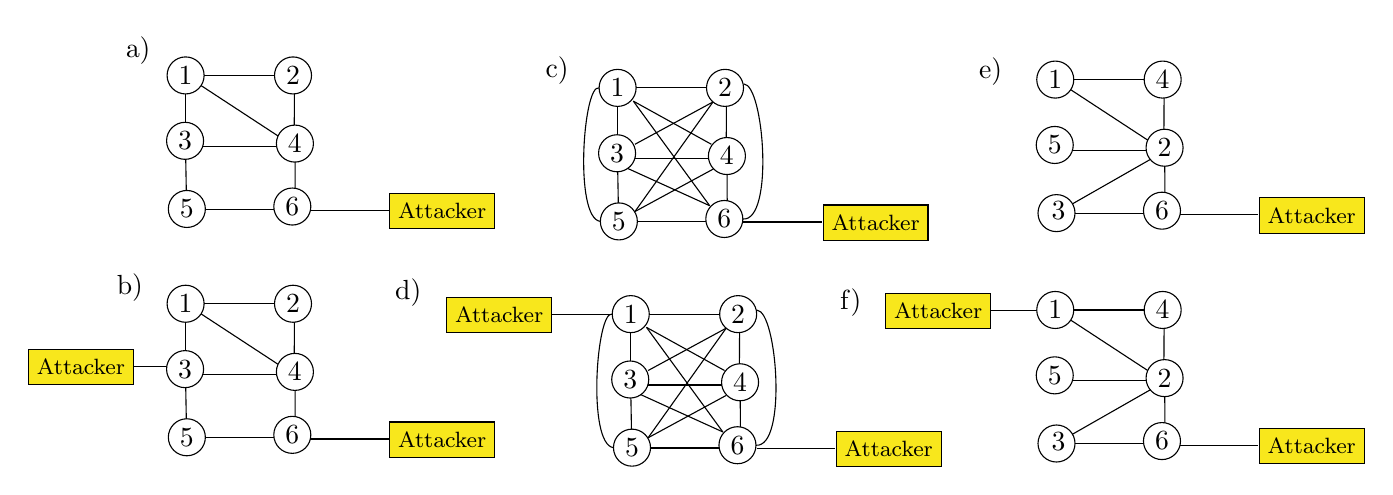
\begin{tikzpicture}[x=0.75pt,y=0.75pt,yscale=-1,xscale=1]
%uncomment if require: \path (0,300); %set diagram left start at 0, and has height of 300

%Straight Lines [id:da21270339539187544] 
\draw    (50.75,166.4) -- (88.67,166.4) ;


%Shape: Rectangle [id:dp19806528063640816] 
\draw  [fill={rgb, 255:red, 248; green, 231; blue, 28 }  ,fill opacity=1 ] (9.2,158.2) -- (59.67,158.2) -- (59.67,175.18) -- (9.2,175.18) -- cycle ;


%Straight Lines [id:da3153834125753151] 
\draw    (137.33,132.22) -- (137.17,163.81) ;


%Straight Lines [id:da7084115546458901] 
\draw    (91.08,200.73) -- (129,200.73) ;


%Straight Lines [id:da9623839826112595] 
\draw    (84.83,136.23) -- (140.58,172.73) ;


%Straight Lines [id:da2909368745777172] 
\draw    (84.83,172.73) -- (85.33,200.55) ;


%Straight Lines [id:da35867881660722734] 
\draw    (137.58,170.73) -- (137.67,202.88) ;


%Shape: Circle [id:dp9939759302306557] 
\draw  [fill={rgb, 255:red, 255; green, 255; blue, 255 }  ,fill opacity=1 ] (75.92,136.23) .. controls (75.92,131.3) and (79.91,127.31) .. (84.83,127.31) .. controls (89.76,127.31) and (93.75,131.3) .. (93.75,136.23) .. controls (93.75,141.15) and (89.76,145.15) .. (84.83,145.15) .. controls (79.91,145.15) and (75.92,141.15) .. (75.92,136.23) -- cycle ;

%Shape: Circle [id:dp34760301125310855] 
\draw  [fill={rgb, 255:red, 255; green, 255; blue, 255 }  ,fill opacity=1 ] (128.58,169.06) .. controls (128.58,164.14) and (132.58,160.15) .. (137.5,160.15) .. controls (142.42,160.15) and (146.42,164.14) .. (146.42,169.06) .. controls (146.42,173.99) and (142.42,177.98) .. (137.5,177.98) .. controls (132.58,177.98) and (128.58,173.99) .. (128.58,169.06) -- cycle ;

%Shape: Circle [id:dp9702116004071654] 
\draw  [fill={rgb, 255:red, 255; green, 255; blue, 255 }  ,fill opacity=1 ] (127.33,199.4) .. controls (127.33,194.47) and (131.33,190.48) .. (136.25,190.48) .. controls (141.17,190.48) and (145.17,194.47) .. (145.17,199.4) .. controls (145.17,204.32) and (141.17,208.31) .. (136.25,208.31) .. controls (131.33,208.31) and (127.33,204.32) .. (127.33,199.4) -- cycle ;

%Straight Lines [id:da8265544446705831] 
\draw    (93.75,136.23) -- (131.67,136.23) ;


%Straight Lines [id:da1435228669726185] 
\draw    (90.75,170.4) -- (128.67,170.4) ;


%Straight Lines [id:da5512583348761163] 
\draw    (84.83,145.15) -- (84.83,163.81) ;


%Shape: Circle [id:dp33954226442737345] 
\draw  [fill={rgb, 255:red, 255; green, 255; blue, 255 }  ,fill opacity=1 ] (76.52,200.56) .. controls (76.52,195.64) and (80.51,191.65) .. (85.43,191.65) .. controls (90.36,191.65) and (94.35,195.64) .. (94.35,200.56) .. controls (94.35,205.49) and (90.36,209.48) .. (85.43,209.48) .. controls (80.51,209.48) and (76.52,205.49) .. (76.52,200.56) -- cycle ;

%Shape: Circle [id:dp027045110799332694] 
\draw  [fill={rgb, 255:red, 255; green, 255; blue, 255 }  ,fill opacity=1 ] (75.67,167.73) .. controls (75.67,162.8) and (79.66,158.81) .. (84.58,158.81) .. controls (89.51,158.81) and (93.5,162.8) .. (93.5,167.73) .. controls (93.5,172.65) and (89.51,176.65) .. (84.58,176.65) .. controls (79.66,176.65) and (75.67,172.65) .. (75.67,167.73) -- cycle ;

%Shape: Circle [id:dp8622510797031577] 
\draw  [fill={rgb, 255:red, 255; green, 255; blue, 255 }  ,fill opacity=1 ] (127.67,136.23) .. controls (127.67,131.3) and (131.66,127.31) .. (136.58,127.31) .. controls (141.51,127.31) and (145.5,131.3) .. (145.5,136.23) .. controls (145.5,141.15) and (141.51,145.15) .. (136.58,145.15) .. controls (131.66,145.15) and (127.67,141.15) .. (127.67,136.23) -- cycle ;

%Straight Lines [id:da8162398929728556] 
\draw    (144.75,201.4) -- (182.67,201.4) ;


%Shape: Rectangle [id:dp15602990655598958] 
\draw  [fill={rgb, 255:red, 248; green, 231; blue, 28 }  ,fill opacity=1 ] (183.2,193.2) -- (233.67,193.2) -- (233.67,210.18) -- (183.2,210.18) -- cycle ;




%Straight Lines [id:da675337569741544] 
\draw    (137.33,22.22) -- (137.17,53.81) ;


%Straight Lines [id:da9770217193149313] 
\draw    (91.08,90.73) -- (129,90.73) ;


%Straight Lines [id:da18857026751215256] 
\draw    (84.83,26.23) -- (140.58,62.73) ;


%Straight Lines [id:da6275844068359788] 
\draw    (84.83,62.73) -- (85.33,90.55) ;


%Straight Lines [id:da3859409733288094] 
\draw    (137.58,60.73) -- (137.67,92.88) ;


%Shape: Circle [id:dp38555186789719464] 
\draw  [fill={rgb, 255:red, 255; green, 255; blue, 255 }  ,fill opacity=1 ] (75.92,26.23) .. controls (75.92,21.3) and (79.91,17.31) .. (84.83,17.31) .. controls (89.76,17.31) and (93.75,21.3) .. (93.75,26.23) .. controls (93.75,31.15) and (89.76,35.15) .. (84.83,35.15) .. controls (79.91,35.15) and (75.92,31.15) .. (75.92,26.23) -- cycle ;

%Shape: Circle [id:dp6614919206504822] 
\draw  [fill={rgb, 255:red, 255; green, 255; blue, 255 }  ,fill opacity=1 ] (128.58,59.06) .. controls (128.58,54.14) and (132.58,50.15) .. (137.5,50.15) .. controls (142.42,50.15) and (146.42,54.14) .. (146.42,59.06) .. controls (146.42,63.99) and (142.42,67.98) .. (137.5,67.98) .. controls (132.58,67.98) and (128.58,63.99) .. (128.58,59.06) -- cycle ;

%Shape: Circle [id:dp4792028510349877] 
\draw  [fill={rgb, 255:red, 255; green, 255; blue, 255 }  ,fill opacity=1 ] (127.33,89.4) .. controls (127.33,84.47) and (131.33,80.48) .. (136.25,80.48) .. controls (141.17,80.48) and (145.17,84.47) .. (145.17,89.4) .. controls (145.17,94.32) and (141.17,98.31) .. (136.25,98.31) .. controls (131.33,98.31) and (127.33,94.32) .. (127.33,89.4) -- cycle ;

%Straight Lines [id:da5503390690988923] 
\draw    (93.75,26.23) -- (131.67,26.23) ;


%Straight Lines [id:da4684291204598492] 
\draw    (90.75,60.4) -- (128.67,60.4) ;


%Straight Lines [id:da14625515615077633] 
\draw    (84.83,35.15) -- (84.83,53.81) ;


%Shape: Circle [id:dp5312971223005962] 
\draw  [fill={rgb, 255:red, 255; green, 255; blue, 255 }  ,fill opacity=1 ] (76.52,90.56) .. controls (76.52,85.64) and (80.51,81.65) .. (85.43,81.65) .. controls (90.36,81.65) and (94.35,85.64) .. (94.35,90.56) .. controls (94.35,95.49) and (90.36,99.48) .. (85.43,99.48) .. controls (80.51,99.48) and (76.52,95.49) .. (76.52,90.56) -- cycle ;

%Shape: Circle [id:dp8123330510491519] 
\draw  [fill={rgb, 255:red, 255; green, 255; blue, 255 }  ,fill opacity=1 ] (75.67,57.73) .. controls (75.67,52.8) and (79.66,48.81) .. (84.58,48.81) .. controls (89.51,48.81) and (93.5,52.8) .. (93.5,57.73) .. controls (93.5,62.65) and (89.51,66.65) .. (84.58,66.65) .. controls (79.66,66.65) and (75.67,62.65) .. (75.67,57.73) -- cycle ;

%Shape: Circle [id:dp008503760549775086] 
\draw  [fill={rgb, 255:red, 255; green, 255; blue, 255 }  ,fill opacity=1 ] (127.67,26.23) .. controls (127.67,21.3) and (131.66,17.31) .. (136.58,17.31) .. controls (141.51,17.31) and (145.5,21.3) .. (145.5,26.23) .. controls (145.5,31.15) and (141.51,35.15) .. (136.58,35.15) .. controls (131.66,35.15) and (127.67,31.15) .. (127.67,26.23) -- cycle ;

%Straight Lines [id:da5256421122460654] 
\draw    (144.75,91.4) -- (182.67,91.4) ;


%Shape: Rectangle [id:dp7797605979818211] 
\draw  [fill={rgb, 255:red, 248; green, 231; blue, 28 }  ,fill opacity=1 ] (183.2,83.2) -- (233.67,83.2) -- (233.67,100.18) -- (183.2,100.18) -- cycle ;




%Straight Lines [id:da22867619419553487] 
\draw    (345.47,28.22) -- (345.31,59.81) ;


%Straight Lines [id:da7366629057200433] 
\draw    (299.22,96.73) -- (337.14,96.73) ;


%Straight Lines [id:da5560609381608291] 
\draw    (292.97,68.73) -- (293.47,96.55) ;


%Straight Lines [id:da4739025620423759] 
\draw    (345.72,66.73) -- (345.81,98.88) ;


%Shape: Circle [id:dp9922005762933758] 
\draw  [fill={rgb, 255:red, 255; green, 255; blue, 255 }  ,fill opacity=1 ] (284.06,32.23) .. controls (284.06,27.3) and (288.05,23.31) .. (292.97,23.31) .. controls (297.9,23.31) and (301.89,27.3) .. (301.89,32.23) .. controls (301.89,37.15) and (297.9,41.15) .. (292.97,41.15) .. controls (288.05,41.15) and (284.06,37.15) .. (284.06,32.23) -- cycle ;

%Shape: Circle [id:dp7388325613342047] 
\draw  [fill={rgb, 255:red, 255; green, 255; blue, 255 }  ,fill opacity=1 ] (336.72,65.06) .. controls (336.72,60.14) and (340.72,56.15) .. (345.64,56.15) .. controls (350.57,56.15) and (354.56,60.14) .. (354.56,65.06) .. controls (354.56,69.99) and (350.57,73.98) .. (345.64,73.98) .. controls (340.72,73.98) and (336.72,69.99) .. (336.72,65.06) -- cycle ;

%Shape: Circle [id:dp3047262312307377] 
\draw  [fill={rgb, 255:red, 255; green, 255; blue, 255 }  ,fill opacity=1 ] (335.47,95.4) .. controls (335.47,90.47) and (339.47,86.48) .. (344.39,86.48) .. controls (349.32,86.48) and (353.31,90.47) .. (353.31,95.4) .. controls (353.31,100.32) and (349.32,104.31) .. (344.39,104.31) .. controls (339.47,104.31) and (335.47,100.32) .. (335.47,95.4) -- cycle ;

%Straight Lines [id:da5232789861595977] 
\draw    (301.89,32.23) -- (339.81,32.23) ;


%Straight Lines [id:da39641445777079876] 
\draw    (298.89,66.4) -- (336.81,66.4) ;


%Straight Lines [id:da6500529894480953] 
\draw    (292.97,41.15) -- (292.97,59.81) ;


%Shape: Circle [id:dp421295758241513] 
\draw  [fill={rgb, 255:red, 255; green, 255; blue, 255 }  ,fill opacity=1 ] (284.66,96.56) .. controls (284.66,91.64) and (288.65,87.65) .. (293.57,87.65) .. controls (298.5,87.65) and (302.49,91.64) .. (302.49,96.56) .. controls (302.49,101.49) and (298.5,105.48) .. (293.57,105.48) .. controls (288.65,105.48) and (284.66,101.49) .. (284.66,96.56) -- cycle ;

%Shape: Circle [id:dp68993621237352] 
\draw  [fill={rgb, 255:red, 255; green, 255; blue, 255 }  ,fill opacity=1 ] (283.81,63.73) .. controls (283.81,58.8) and (287.8,54.81) .. (292.72,54.81) .. controls (297.65,54.81) and (301.64,58.8) .. (301.64,63.73) .. controls (301.64,68.65) and (297.65,72.65) .. (292.72,72.65) .. controls (287.8,72.65) and (283.81,68.65) .. (283.81,63.73) -- cycle ;

%Shape: Circle [id:dp0004348717523896539] 
\draw  [fill={rgb, 255:red, 255; green, 255; blue, 255 }  ,fill opacity=1 ] (335.81,32.23) .. controls (335.81,27.3) and (339.8,23.31) .. (344.72,23.31) .. controls (349.65,23.31) and (353.64,27.3) .. (353.64,32.23) .. controls (353.64,37.15) and (349.65,41.15) .. (344.72,41.15) .. controls (339.8,41.15) and (335.81,37.15) .. (335.81,32.23) -- cycle ;

%Straight Lines [id:da3470843344836425] 
\draw    (297.74,71) -- (337.34,89) ;


%Straight Lines [id:da22385827339648745] 
\draw    (300.54,38.6) -- (338.14,59.4) ;


%Straight Lines [id:da9470627692324495] 
\draw    (301.34,59.4) -- (338.94,39) ;


%Straight Lines [id:da527163614428479] 
\draw    (301.34,91.8) -- (338.94,71.4) ;


%Curve Lines [id:da2659177622157741] 
\draw    (353.81,30.33) .. controls (363.47,30.67) and (368.47,96.67) .. (353.31,95.4) ;


%Curve Lines [id:da3968887523398855] 
\draw    (284.06,32.23) .. controls (276.47,30) and (271.81,95) .. (284.66,96.56) ;


%Straight Lines [id:da4862470624661749] 
\draw    (300.54,38.6) -- (337.34,89) ;


%Straight Lines [id:da9265421066580971] 
\draw    (338.94,39) -- (301.34,91.8) ;


%Straight Lines [id:da7131649869831252] 
\draw    (353.61,96.82) -- (391.52,96.82) ;


%Shape: Rectangle [id:dp3615803597823173] 
\draw  [fill={rgb, 255:red, 248; green, 231; blue, 28 }  ,fill opacity=1 ] (392.06,88.63) -- (442.53,88.63) -- (442.53,105.61) -- (392.06,105.61) -- cycle ;




%Straight Lines [id:da6715977826012206] 
\draw    (351.81,137.22) -- (351.64,168.81) ;


%Straight Lines [id:da9540657786576023] 
\draw    (305.56,205.73) -- (343.48,205.73) ;


%Straight Lines [id:da5731952874596753] 
\draw    (299.31,177.73) -- (299.81,205.55) ;


%Straight Lines [id:da41041637205710924] 
\draw    (352.06,175.73) -- (352.14,207.88) ;


%Shape: Circle [id:dp7490995910930758] 
\draw  [fill={rgb, 255:red, 255; green, 255; blue, 255 }  ,fill opacity=1 ] (290.39,141.23) .. controls (290.39,136.3) and (294.38,132.31) .. (299.31,132.31) .. controls (304.23,132.31) and (308.23,136.3) .. (308.23,141.23) .. controls (308.23,146.15) and (304.23,150.15) .. (299.31,150.15) .. controls (294.38,150.15) and (290.39,146.15) .. (290.39,141.23) -- cycle ;

%Shape: Circle [id:dp21867347242120194] 
\draw  [fill={rgb, 255:red, 255; green, 255; blue, 255 }  ,fill opacity=1 ] (343.06,174.06) .. controls (343.06,169.14) and (347.05,165.15) .. (351.98,165.15) .. controls (356.9,165.15) and (360.89,169.14) .. (360.89,174.06) .. controls (360.89,178.99) and (356.9,182.98) .. (351.98,182.98) .. controls (347.05,182.98) and (343.06,178.99) .. (343.06,174.06) -- cycle ;

%Shape: Circle [id:dp009688206133991684] 
\draw  [fill={rgb, 255:red, 255; green, 255; blue, 255 }  ,fill opacity=1 ] (341.81,204.4) .. controls (341.81,199.47) and (345.8,195.48) .. (350.73,195.48) .. controls (355.65,195.48) and (359.64,199.47) .. (359.64,204.4) .. controls (359.64,209.32) and (355.65,213.31) .. (350.73,213.31) .. controls (345.8,213.31) and (341.81,209.32) .. (341.81,204.4) -- cycle ;

%Straight Lines [id:da45622560516359056] 
\draw    (308.23,141.23) -- (346.14,141.23) ;


%Straight Lines [id:da8381919416870578] 
\draw    (305.23,175.4) -- (343.14,175.4) ;


%Straight Lines [id:da6163529535308253] 
\draw    (299.31,150.15) -- (299.31,168.81) ;


%Shape: Circle [id:dp456728946120202] 
\draw  [fill={rgb, 255:red, 255; green, 255; blue, 255 }  ,fill opacity=1 ] (290.99,205.56) .. controls (290.99,200.64) and (294.98,196.65) .. (299.91,196.65) .. controls (304.83,196.65) and (308.83,200.64) .. (308.83,205.56) .. controls (308.83,210.49) and (304.83,214.48) .. (299.91,214.48) .. controls (294.98,214.48) and (290.99,210.49) .. (290.99,205.56) -- cycle ;

%Shape: Circle [id:dp45682398029629745] 
\draw  [fill={rgb, 255:red, 255; green, 255; blue, 255 }  ,fill opacity=1 ] (290.14,172.73) .. controls (290.14,167.8) and (294.13,163.81) .. (299.06,163.81) .. controls (303.98,163.81) and (307.98,167.8) .. (307.98,172.73) .. controls (307.98,177.65) and (303.98,181.65) .. (299.06,181.65) .. controls (294.13,181.65) and (290.14,177.65) .. (290.14,172.73) -- cycle ;

%Shape: Circle [id:dp20828836021634367] 
\draw  [fill={rgb, 255:red, 255; green, 255; blue, 255 }  ,fill opacity=1 ] (342.14,141.23) .. controls (342.14,136.3) and (346.13,132.31) .. (351.06,132.31) .. controls (355.98,132.31) and (359.98,136.3) .. (359.98,141.23) .. controls (359.98,146.15) and (355.98,150.15) .. (351.06,150.15) .. controls (346.13,150.15) and (342.14,146.15) .. (342.14,141.23) -- cycle ;

%Straight Lines [id:da32117265204513157] 
\draw    (304.08,180) -- (343.68,198) ;


%Straight Lines [id:da6079841314173954] 
\draw    (306.88,147.6) -- (344.48,168.4) ;


%Straight Lines [id:da7680118845457601] 
\draw    (307.68,168.4) -- (345.28,148) ;


%Straight Lines [id:da6389773826545454] 
\draw    (307.68,200.8) -- (345.28,180.4) ;


%Curve Lines [id:da511824766847756] 
\draw    (360.14,139.33) .. controls (369.81,139.67) and (374.81,205.67) .. (359.64,204.4) ;


%Curve Lines [id:da10840460492754567] 
\draw    (290.39,141.23) .. controls (282.81,139) and (278.14,204) .. (290.99,205.56) ;


%Straight Lines [id:da3147720372519749] 
\draw    (306.88,147.6) -- (343.68,198) ;


%Straight Lines [id:da9757233447370841] 
\draw    (345.28,148) -- (307.68,200.8) ;


%Straight Lines [id:da8351826345519837] 
\draw    (359.94,205.82) -- (397.86,205.82) ;


%Shape: Rectangle [id:dp9492523154356004] 
\draw  [fill={rgb, 255:red, 248; green, 231; blue, 28 }  ,fill opacity=1 ] (398.39,197.63) -- (448.86,197.63) -- (448.86,214.61) -- (398.39,214.61) -- cycle ;


%Straight Lines [id:da7783875840754805] 
\draw    (252.23,141.4) -- (290.14,141.4) ;


%Shape: Rectangle [id:dp8219665960733671] 
\draw  [fill={rgb, 255:red, 248; green, 231; blue, 28 }  ,fill opacity=1 ] (210.68,133.2) -- (261.15,133.2) -- (261.15,150.18) -- (210.68,150.18) -- cycle ;



%Straight Lines [id:da7147269629924605] 
\draw    (556.33,24.22) -- (556.17,55.81) ;


%Straight Lines [id:da8277651830187894] 
\draw    (510.08,92.73) -- (548,92.73) ;


%Straight Lines [id:da0013601110130750937] 
\draw    (503.83,28.23) -- (559.58,64.73) ;


%Straight Lines [id:da5364857137309426] 
\draw    (556.58,62.73) -- (504.33,92.55) ;


%Straight Lines [id:da09227991689524317] 
\draw    (556.58,62.73) -- (556.67,94.88) ;


%Shape: Circle [id:dp40945899905332894] 
\draw  [fill={rgb, 255:red, 255; green, 255; blue, 255 }  ,fill opacity=1 ] (494.92,28.23) .. controls (494.92,23.3) and (498.91,19.31) .. (503.83,19.31) .. controls (508.76,19.31) and (512.75,23.3) .. (512.75,28.23) .. controls (512.75,33.15) and (508.76,37.15) .. (503.83,37.15) .. controls (498.91,37.15) and (494.92,33.15) .. (494.92,28.23) -- cycle ;

%Shape: Circle [id:dp7767184939243962] 
\draw  [fill={rgb, 255:red, 255; green, 255; blue, 255 }  ,fill opacity=1 ] (547.58,61.06) .. controls (547.58,56.14) and (551.58,52.15) .. (556.5,52.15) .. controls (561.42,52.15) and (565.42,56.14) .. (565.42,61.06) .. controls (565.42,65.99) and (561.42,69.98) .. (556.5,69.98) .. controls (551.58,69.98) and (547.58,65.99) .. (547.58,61.06) -- cycle ;
%Shape: Circle [id:dp4692699516703288] 
\draw  [fill={rgb, 255:red, 255; green, 255; blue, 255 }  ,fill opacity=1 ] (546.33,91.4) .. controls (546.33,86.47) and (550.33,82.48) .. (555.25,82.48) .. controls (560.17,82.48) and (564.17,86.47) .. (564.17,91.4) .. controls (564.17,96.32) and (560.17,100.31) .. (555.25,100.31) .. controls (550.33,100.31) and (546.33,96.32) .. (546.33,91.4) -- cycle ;

%Straight Lines [id:da9597316941694047] 
\draw    (512.75,28.23) -- (550.67,28.23) ;


%Straight Lines [id:da7708545450116795] 
\draw    (509.75,62.4) -- (547.67,62.4) ;


%Shape: Circle [id:dp40660215241265885] 
\draw  [fill={rgb, 255:red, 255; green, 255; blue, 255 }  ,fill opacity=1 ] (495.52,92.56) .. controls (495.52,87.64) and (499.51,83.65) .. (504.43,83.65) .. controls (509.36,83.65) and (513.35,87.64) .. (513.35,92.56) .. controls (513.35,97.49) and (509.36,101.48) .. (504.43,101.48) .. controls (499.51,101.48) and (495.52,97.49) .. (495.52,92.56) -- cycle ;
%Shape: Circle [id:dp09457558597010363] 
\draw  [fill={rgb, 255:red, 255; green, 255; blue, 255 }  ,fill opacity=1 ] (494.67,59.73) .. controls (494.67,54.8) and (498.66,50.81) .. (503.58,50.81) .. controls (508.51,50.81) and (512.5,54.8) .. (512.5,59.73) .. controls (512.5,64.65) and (508.51,68.65) .. (503.58,68.65) .. controls (498.66,68.65) and (494.67,64.65) .. (494.67,59.73) -- cycle ;
%Shape: Circle [id:dp7445040256787864] 
\draw  [fill={rgb, 255:red, 255; green, 255; blue, 255 }  ,fill opacity=1 ] (546.67,28.23) .. controls (546.67,23.3) and (550.66,19.31) .. (555.58,19.31) .. controls (560.51,19.31) and (564.5,23.3) .. (564.5,28.23) .. controls (564.5,33.15) and (560.51,37.15) .. (555.58,37.15) .. controls (550.66,37.15) and (546.67,33.15) .. (546.67,28.23) -- cycle ;
%Straight Lines [id:da6980179493369204] 
\draw    (563.75,93.4) -- (601.67,93.4) ;


%Shape: Rectangle [id:dp9981691173299058] 
\draw  [fill={rgb, 255:red, 248; green, 231; blue, 28 }  ,fill opacity=1 ] (602.2,85.2) -- (652.67,85.2) -- (652.67,102.18) -- (602.2,102.18) -- cycle ;




%Straight Lines [id:da8092387671610324] 
\draw    (463.75,139.4) -- (501.67,139.4) ;


%Shape: Rectangle [id:dp7958055249044546] 
\draw  [fill={rgb, 255:red, 248; green, 231; blue, 28 }  ,fill opacity=1 ] (422.2,131.2) -- (472.67,131.2) -- (472.67,148.18) -- (422.2,148.18) -- cycle ;


%Straight Lines [id:da8513354272469744] 
\draw    (556.33,135.22) -- (556.17,166.81) ;


%Straight Lines [id:da7992137672953211] 
\draw    (510.08,203.73) -- (548,203.73) ;


%Straight Lines [id:da3954660742507915] 
\draw    (503.83,139.23) -- (559.58,175.73) ;


%Straight Lines [id:da5825560768425334] 
\draw    (556.58,173.73) -- (504.33,203.55) ;


%Straight Lines [id:da5568053188323774] 
\draw    (556.58,173.73) -- (556.67,205.88) ;


%Shape: Circle [id:dp30253748945575554] 
\draw  [fill={rgb, 255:red, 255; green, 255; blue, 255 }  ,fill opacity=1 ] (494.92,139.23) .. controls (494.92,134.3) and (498.91,130.31) .. (503.83,130.31) .. controls (508.76,130.31) and (512.75,134.3) .. (512.75,139.23) .. controls (512.75,144.15) and (508.76,148.15) .. (503.83,148.15) .. controls (498.91,148.15) and (494.92,144.15) .. (494.92,139.23) -- cycle ;

%Shape: Circle [id:dp3641428183407782] 
\draw  [fill={rgb, 255:red, 255; green, 255; blue, 255 }  ,fill opacity=1 ] (547.58,172.06) .. controls (547.58,167.14) and (551.58,163.15) .. (556.5,163.15) .. controls (561.42,163.15) and (565.42,167.14) .. (565.42,172.06) .. controls (565.42,176.99) and (561.42,180.98) .. (556.5,180.98) .. controls (551.58,180.98) and (547.58,176.99) .. (547.58,172.06) -- cycle ;
%Shape: Circle [id:dp08738614749957285] 
\draw  [fill={rgb, 255:red, 255; green, 255; blue, 255 }  ,fill opacity=1 ] (546.33,202.4) .. controls (546.33,197.47) and (550.33,193.48) .. (555.25,193.48) .. controls (560.17,193.48) and (564.17,197.47) .. (564.17,202.4) .. controls (564.17,207.32) and (560.17,211.31) .. (555.25,211.31) .. controls (550.33,211.31) and (546.33,207.32) .. (546.33,202.4) -- cycle ;

%Straight Lines [id:da8382293979078496] 
\draw    (512.75,139.23) -- (550.67,139.23) ;


%Straight Lines [id:da06888701209203096] 
\draw    (509.75,173.4) -- (547.67,173.4) ;


%Shape: Circle [id:dp03475136247746857] 
\draw  [fill={rgb, 255:red, 255; green, 255; blue, 255 }  ,fill opacity=1 ] (495.52,203.56) .. controls (495.52,198.64) and (499.51,194.65) .. (504.43,194.65) .. controls (509.36,194.65) and (513.35,198.64) .. (513.35,203.56) .. controls (513.35,208.49) and (509.36,212.48) .. (504.43,212.48) .. controls (499.51,212.48) and (495.52,208.49) .. (495.52,203.56) -- cycle ;
%Shape: Circle [id:dp825936328113765] 
\draw  [fill={rgb, 255:red, 255; green, 255; blue, 255 }  ,fill opacity=1 ] (494.67,170.73) .. controls (494.67,165.8) and (498.66,161.81) .. (503.58,161.81) .. controls (508.51,161.81) and (512.5,165.8) .. (512.5,170.73) .. controls (512.5,175.65) and (508.51,179.65) .. (503.58,179.65) .. controls (498.66,179.65) and (494.67,175.65) .. (494.67,170.73) -- cycle ;
%Shape: Circle [id:dp10791744420385518] 
\draw  [fill={rgb, 255:red, 255; green, 255; blue, 255 }  ,fill opacity=1 ] (546.67,139.23) .. controls (546.67,134.3) and (550.66,130.31) .. (555.58,130.31) .. controls (560.51,130.31) and (564.5,134.3) .. (564.5,139.23) .. controls (564.5,144.15) and (560.51,148.15) .. (555.58,148.15) .. controls (550.66,148.15) and (546.67,144.15) .. (546.67,139.23) -- cycle ;
%Straight Lines [id:da35173459455787404] 
\draw    (563.75,204.4) -- (601.67,204.4) ;


%Shape: Rectangle [id:dp6910000106247179] 
\draw  [fill={rgb, 255:red, 248; green, 231; blue, 28 }  ,fill opacity=1 ] (602.2,196.2) -- (652.67,196.2) -- (652.67,213.18) -- (602.2,213.18) -- cycle ;




% Text Node
\draw (405.33,135.67) node  [align=left] {f)};
% Text Node
\draw (556.5,172.06) node  [align=left] {2};
% Text Node
\draw (505.43,202.56) node  [align=left] {3};
% Text Node
\draw (503.58,170.73) node  [align=left] {5};
% Text Node
\draw (555.58,139.23) node  [align=left] {4};
% Text Node
\draw (627.44,204.69) node  [align=left] {{\footnotesize Attacker}};
% Text Node
\draw (555.25,202.4) node  [align=left] {6};
% Text Node
\draw (503.83,139.23) node  [align=left] {1};
% Text Node
\draw (447.44,139.69) node  [align=left] {{\footnotesize Attacker}};
% Text Node
\draw (472.67,24.33) node  [align=left] {e)};
% Text Node
\draw (556.5,61.06) node  [align=left] {2};
% Text Node
\draw (505.43,91.56) node  [align=left] {3};
% Text Node
\draw (503.58,59.73) node  [align=left] {5};
% Text Node
\draw (555.58,28.23) node  [align=left] {4};
% Text Node
\draw (627.44,93.69) node  [align=left] {{\footnotesize Attacker}};
% Text Node
\draw (555.25,91.4) node  [align=left] {6};
% Text Node
\draw (503.83,28.23) node  [align=left] {1};
% Text Node
\draw (192.14,131) node  [align=left] {d)};
% Text Node
\draw (235.91,141.69) node  [align=left] {{\footnotesize Attacker}};
% Text Node
\draw (423.63,206.12) node  [align=left] {{\footnotesize Attacker}};
% Text Node
\draw (351.06,141.23) node  [align=left] {2};
% Text Node
\draw (299.06,172.73) node  [align=left] {3};
% Text Node
\draw (299.91,205.56) node  [align=left] {5};
% Text Node
\draw (350.73,204.4) node  [align=left] {6};
% Text Node
\draw (351.98,174.06) node  [align=left] {4};
% Text Node
\draw (299.31,141.23) node  [align=left] {1};
% Text Node
\draw (263.81,24) node  [align=left] {c)};
% Text Node
\draw (417.29,97.12) node  [align=left] {{\footnotesize Attacker}};
% Text Node
\draw (344.72,32.23) node  [align=left] {2};
% Text Node
\draw (292.72,63.73) node  [align=left] {3};
% Text Node
\draw (293.57,96.56) node  [align=left] {5};
% Text Node
\draw (344.39,95.4) node  [align=left] {6};
% Text Node
\draw (345.64,65.06) node  [align=left] {4};
% Text Node
\draw (292.97,32.23) node  [align=left] {1};
% Text Node
\draw (62,14.33) node  [align=left] {a)};
% Text Node
\draw (208.44,91.69) node  [align=left] {{\footnotesize Attacker}};
% Text Node
\draw (136.58,26.23) node  [align=left] {2};
% Text Node
\draw (84.58,57.73) node  [align=left] {3};
% Text Node
\draw (85.43,90.56) node  [align=left] {5};
% Text Node
\draw (136.25,89.4) node  [align=left] {6};
% Text Node
\draw (137.5,59.06) node  [align=left] {4};
% Text Node
\draw (84.83,26.23) node  [align=left] {1};
% Text Node
\draw (58,128.33) node  [align=left] {b)};
% Text Node
\draw (208.44,201.69) node  [align=left] {{\footnotesize Attacker}};
% Text Node
\draw (136.58,136.23) node  [align=left] {2};
% Text Node
\draw (84.58,167.73) node  [align=left] {3};
% Text Node
\draw (85.43,200.56) node  [align=left] {5};
% Text Node
\draw (136.25,199.4) node  [align=left] {6};
% Text Node
\draw (137.5,169.06) node  [align=left] {4};
% Text Node
\draw (84.83,136.23) node  [align=left] {1};
% Text Node
\draw (34.44,166.69) node  [align=left] {{\footnotesize Attacker}};


\end{tikzpicture}


\caption{Use case topologies}
\label{fig:mdp-usecase-single}
\end{figure}
 
We migrate a Virtual Network where the target substrate will be composed of physical nodes 1, 2 and 3.
Node 6 is the exfiltration point of the attacker, which means that the attacker will establish a path between node 6 and one of the nodes embedding the Virtual Network (\ie node 1, node 2 and/or node 3).
% In order to make the generation of the MDP states computationally tractable, we set a constant impact performance on all nodes. 
We set the discount factor of the value iteration algorithm to 0.9, a common value for use cases found in the literature.
We set $\alpha=0.7$, the probability of an attack being launched during the next transition.
We set $\beta=3$ the weight factor to target nodes supporting the embedding.
We set the intrinsic value $V$ of the nodes embedding the Virtual Network (nodes 1, 2 and 3) to be higher than the others (nodes 4, 5 and 6) because they will operate the virtual network.

We summarize these parameters in Table~\ref{tab:mdp-parameters}. 
% \CK{Precise que le choix des Vi est en accord avec le fait que les noeuds qui sont les cibles de l'embedding sont plus importants. Par ailleurs, pourquoi $c_c^j = 10$ partout ? Le cout est cense etre proportionnel a Vj non ?}
We compute the optimal policy of each MDP using MDPToolbox~\cite{Chades2014} and the Value Iteration algorithm~\cite{bellman1957}.

\begin{table}[ht]
\centering
\begin{tabular}{|c|c|l|c|c|c|c|}
\hline
$\alpha$ & \multicolumn{2}{c|}{$\beta$} & Exfiltration point & $c_f$ & $k_c$ & $\gamma$ \\ \hline
0.7      & \multicolumn{2}{c|}{3}       & Node 6             & 10    & 1    & 0.9      \\ \hline
\multicolumn{7}{|c|}{$V_1=10,V_2=10,V_3=10,V_4=5,V_5=5,V_6=5$}                          \\ \hline
\multicolumn{7}{|c|}{$c_c^1=10,c_c^2=10,c_c^3=10,c_c^4=5,c_c^5=5,c_c^6=5$}                          \\ \hline
\multicolumn{7}{|c|}{Physical embedding: Nodes 1 - Node 2 - Node 3}                     \\ \hline
\multicolumn{7}{|c|}{Migration order: 1 $\rightarrow$ 2 $\rightarrow$ 3}                \\ \hline
\end{tabular}
\caption{Use cases parameters}
\label{tab:mdp-parameters}
\end{table}



We run the MDP using different budgets and detection probabilities.
The time required to fully migrate the VN is $b_f=30$, but we explore use cases with a budget $b_f=40$ that gives more time for the attacker to compromise the infrastructure. We considered that the attacker exploits vulnerabilities that are not limited to the migration process, thus he may continue his attacks beyond the end of the migration. We discuss some implications and limitations of this assumption in Section~\ref{sec:mdp-discussion}.

The ordering of the nodes impacts the result sets of Algorithm~\ref{algo:target}, thus which nodes may be attacked at each transition.
Details about the attack source node for attacks against the migration are summarized in Table~\ref{tab:mdp-attack-source}. Each node in the \textbf{Target node} row will be attacked from the corresponding \textbf{Attack source}.

% Please add the following required packages to your document preamble:
% \usepackage{graphicx}
\begin{table}[h]
\resizebox{\textwidth}{!}{%
\begin{tabular}{|c|c|c|c|c|c|c|c|c|c|c|c|c|c|c|c|c|c|c|c|c|c|c|}
\cline{1-7} \cline{9-15} \cline{17-23}
\multicolumn{7}{|c|}{\textbf{Scenario b)}} &  & \multicolumn{7}{c|}{\textbf{Scenario d)}} &  & \multicolumn{7}{c|}{\textbf{Scenario f)}} \\ \cline{1-7} \cline{9-15} \cline{17-23} 
\textbf{Target node}    & 1  & 2  & 3  & 4  & 5 & 6 &  & \textbf{Target node}    & 1  & 2  & 3  & 4 & 5 & 6 &  & \textbf{Target node}    & 1  & 2  & 3  & 4 & 5 & 6 \\ \cline{1-7} \cline{9-15} \cline{17-23} 
\textbf{Attack source}  & 6  & 4  & 6  & 4  & 6 & 6 &  & \textbf{Attack source}  & 6  & 6  & 1  & 6 & 1 & 1 &  & \textbf{Attack source}  & 6  & 6  & 1  & 6 & 1 & 1 \\ \cline{1-7} \cline{9-15} \cline{17-23} 
\end{tabular}%
}
\caption{Attack sources for multiple attackers scenarios}
\label{tab:mdp-attack-source}
\end{table}

\subsection{Reward of the monitoring set}
We have extracted the monitoring set of each absorbing state, and evaluated the overall reward of each monitoring set and each node individually.
We note $R(Mo)$ the reward of a monitoring set as the sum of the rewards of each corresponding absorbing state.
We also note the reward of a state (resp. a node) $R(State)$ (resp. $R(Node)$). Note however that this reward is different from the reward of an action in an MDP.

Let $S^{\text{Mo}}_{\text{abs}}$ be the set of absorbing states with a common  monitoring set $Mo$, $\rho(Mo)$ the percentage of presence of set $Mo$ in the global solution space and $R(s)$ the reward of state $s$.

\begin{equation}
    R(Mo) = \sum\limits_{s \in S^{\text{Mo}}_{\text{abs}}}\rho(Mo^s)R(s)
\end{equation}


The reward of an absorbing state $R(s)$ is the sum of the reward of each path $p$ in the MDP from the initial state and leading to the absorbing state $s$ times the percentage of presence of the $p$ in the solution space. 
Similarly, the reward of one node in the monitoring set is defined as the sum of the reward of each absorbing state where the chosen node is monitoring the infrastructure.

We illustrate these rewards in Figure~\ref{fig:absstate_reward}, where the initial state is $S_1$ and there are three absorbing states $S_4,S_5$ and $S_6$. Each state yields a reward $r_x$ with a transition probability $p_x$.
State $S_5$ is reached by two paths thus its rewards is the sum of the rewards given by each path.
% The weighted reward uses the stationary distribution of the Markov Chain corresponding to the optimal policy.
If $S_4$ and $S_6$ have the same monitoring set (\ie $Mo^{S_4} = Mo^{S_6}$), then $R(Mo^{S_4}) = R(Mo^{S_6}) = R(S_4) + R(S_6)$.
\begin{figure}[h]

\tikzset{every picture/.style={line width=0.75pt}} %set default line width to 0.75pt        

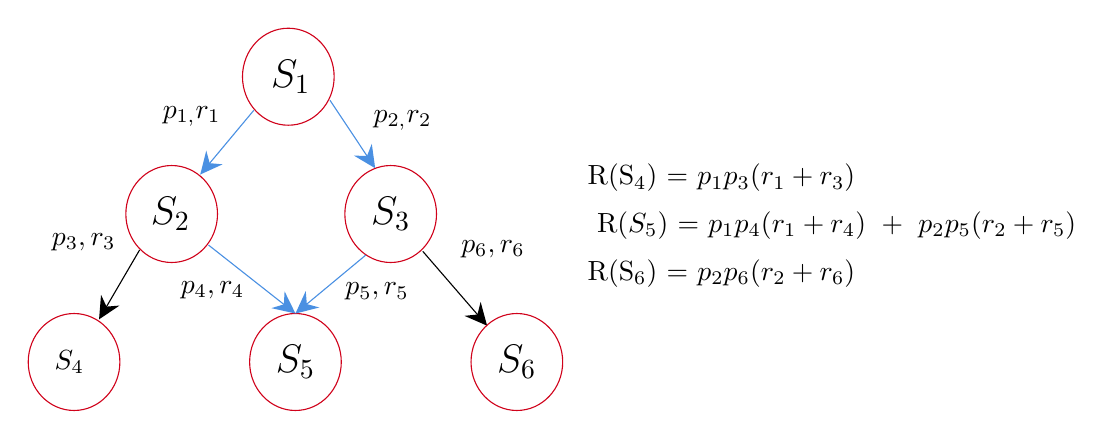
\begin{tikzpicture}[x=0.75pt,y=0.75pt,yscale=-1,xscale=1]
%uncomment if require: \path (0,701.1666717529297); %set diagram left start at 0, and has height of 701.1666717529297

%Straight Lines [id:da8481931635460052] 
\draw    (237.61,125.34) -- (266.62,158.87) ;
\draw [shift={(268.58,161.14)}, rotate = 229.14] [fill={rgb, 255:red, 0; green, 0; blue, 0 }  ][line width=0.08]  [draw opacity=0] (10.72,-5.15) -- (0,0) -- (10.72,5.15) -- (7.12,0) -- cycle    ;

%Shape: Ellipse [id:dp5338816690194331] 
\draw  [color={rgb, 255:red, 208; green, 2; blue, 27 }  ,draw opacity=1 ] (150.73,41.2) .. controls (150.73,28.29) and (160.61,17.83) .. (172.81,17.83) .. controls (185,17.83) and (194.89,28.29) .. (194.89,41.2) .. controls (194.89,54.1) and (185,64.56) .. (172.81,64.56) .. controls (160.61,64.56) and (150.73,54.1) .. (150.73,41.2) -- cycle ;
%Shape: Ellipse [id:dp08323298529021306] 
\draw  [color={rgb, 255:red, 208; green, 2; blue, 27 }  ,draw opacity=1 ] (94.53,107.34) .. controls (94.53,94.44) and (104.41,83.98) .. (116.61,83.98) .. controls (128.8,83.98) and (138.69,94.44) .. (138.69,107.34) .. controls (138.69,120.24) and (128.8,130.7) .. (116.61,130.7) .. controls (104.41,130.7) and (94.53,120.24) .. (94.53,107.34) -- cycle ;
%Shape: Ellipse [id:dp5782501569753735] 
\draw  [color={rgb, 255:red, 208; green, 2; blue, 27 }  ,draw opacity=1 ] (200.05,107.34) .. controls (200.05,94.44) and (209.94,83.98) .. (222.13,83.98) .. controls (234.32,83.98) and (244.21,94.44) .. (244.21,107.34) .. controls (244.21,120.24) and (234.32,130.7) .. (222.13,130.7) .. controls (209.94,130.7) and (200.05,120.24) .. (200.05,107.34) -- cycle ;
%Shape: Ellipse [id:dp9542564413163499] 
\draw  [color={rgb, 255:red, 208; green, 2; blue, 27 }  ,draw opacity=1 ] (47.5,178.64) .. controls (47.5,165.74) and (57.39,155.28) .. (69.58,155.28) .. controls (81.77,155.28) and (91.66,165.74) .. (91.66,178.64) .. controls (91.66,191.54) and (81.77,202) .. (69.58,202) .. controls (57.39,202) and (47.5,191.54) .. (47.5,178.64) -- cycle ;
%Shape: Ellipse [id:dp5730745954231323] 
\draw  [color={rgb, 255:red, 208; green, 2; blue, 27 }  ,draw opacity=1 ] (154.17,178.64) .. controls (154.17,165.74) and (164.06,155.28) .. (176.25,155.28) .. controls (188.44,155.28) and (198.33,165.74) .. (198.33,178.64) .. controls (198.33,191.54) and (188.44,202) .. (176.25,202) .. controls (164.06,202) and (154.17,191.54) .. (154.17,178.64) -- cycle ;
%Shape: Ellipse [id:dp08303160892055261] 
\draw  [color={rgb, 255:red, 208; green, 2; blue, 27 }  ,draw opacity=1 ] (260.84,178.64) .. controls (260.84,165.74) and (270.73,155.28) .. (282.92,155.28) .. controls (295.11,155.28) and (305,165.74) .. (305,178.64) .. controls (305,191.54) and (295.11,202) .. (282.92,202) .. controls (270.73,202) and (260.84,191.54) .. (260.84,178.64) -- cycle ;
%Straight Lines [id:da4561249701318062] 
\draw    (101.12,124.73) -- (83.14,155.52) ;
\draw [shift={(81.62,158.11)}, rotate = 300.3] [fill={rgb, 255:red, 0; green, 0; blue, 0 }  ][line width=0.08]  [draw opacity=0] (10.72,-5.15) -- (0,0) -- (10.72,5.15) -- (7.12,0) -- cycle    ;

%Straight Lines [id:da9228601228550033] 
\draw [color={rgb, 255:red, 74; green, 144; blue, 226 }  ,draw opacity=1 ]   (156.18,57.38) -- (132.29,86.02) ;
\draw [shift={(130.37,88.32)}, rotate = 309.83000000000004] [fill={rgb, 255:red, 74; green, 144; blue, 226 }  ,fill opacity=1 ][line width=0.08]  [draw opacity=0] (10.72,-5.15) -- (0,0) -- (10.72,5.15) -- (7.12,0) -- cycle    ;

%Straight Lines [id:da9215912823895637] 
\draw [color={rgb, 255:red, 74; green, 144; blue, 226 }  ,draw opacity=1 ]   (192.88,52.52) -- (213.01,82.79) ;
\draw [shift={(214.67,85.29)}, rotate = 236.37] [fill={rgb, 255:red, 74; green, 144; blue, 226 }  ,fill opacity=1 ][line width=0.08]  [draw opacity=0] (10.72,-5.15) -- (0,0) -- (10.72,5.15) -- (7.12,0) -- cycle    ;

%Straight Lines [id:da7144026507506241] 
\draw [color={rgb, 255:red, 74; green, 144; blue, 226 }  ,draw opacity=1 ]   (173.89,153.42) -- (134.38,122.31) ;

\draw [shift={(176.25,155.28)}, rotate = 218.22] [fill={rgb, 255:red, 74; green, 144; blue, 226 }  ,fill opacity=1 ][line width=0.08]  [draw opacity=0] (10.72,-5.15) -- (0,0) -- (10.72,5.15) -- (7.12,0) -- cycle    ;
%Straight Lines [id:da10186496684327384] 
\draw [color={rgb, 255:red, 74; green, 144; blue, 226 }  ,draw opacity=1 ]   (178.56,153.36) -- (210.09,127.16) ;

\draw [shift={(176.25,155.28)}, rotate = 320.28] [fill={rgb, 255:red, 74; green, 144; blue, 226 }  ,fill opacity=1 ][line width=0.08]  [draw opacity=0] (10.72,-5.15) -- (0,0) -- (10.72,5.15) -- (7.12,0) -- cycle    ;

% Text Node
\draw (126.24,60.45) node   [align=left] {$\displaystyle p_{1,} r_{1}$};
% Text Node
\draw (227.86,62.45) node   [align=left] {$\displaystyle p_{2,} r_{2}$};
% Text Node
\draw (74.2,121.01) node   [align=left] {$\displaystyle p_{3} ,r_{3}$};
% Text Node
\draw (136.32,143.95) node   [align=left] {$\displaystyle p_{4} ,r_{4}$};
% Text Node
\draw (215.59,144.73) node   [align=left] {$\displaystyle p_{5} ,r_{5}$};
% Text Node
\draw (271.44,124.44) node   [align=left] {$\displaystyle p_{6} ,r_{6}$};
% Text Node
\draw (67.29,178.64) node   [align=left] {$\displaystyle S_{4}$};
% Text Node
\draw (176.25,178.64) node   [align=left] {{\Large $\displaystyle S_{5}$}};
% Text Node
\draw (282.92,178.64) node   [align=left] {{\Large $\displaystyle S_{6}$}};
% Text Node
\draw (116.03,107.34) node  [font=\Large] [align=left] {$\displaystyle S_{2}$};
% Text Node
\draw (222.13,107.34) node  [font=\Large] [align=left] {$\displaystyle S_{3}$};
% Text Node
\draw (173.96,41.2) node  [font=\Large] [align=left] {$\displaystyle S_{1}$};
% Text Node
\draw (381.5,90) node   {R(S$\displaystyle _{4}$) = $\displaystyle p_{1} p_{3}( r_{1} +r_{3})$};
% Text Node
\draw (437,113) node   {R($\displaystyle S_{5}$) = $\displaystyle p_{1} p_{4}( r_{1} +r_{4}) \ +\ p_{2} p_{5}( r_{2} +r_{5})$};
% Text Node
\draw (381.5,136) node   {R(S$\displaystyle _{6}$) = $\displaystyle p_{2} p_{6}( r_{2} +r_{6})$};


\end{tikzpicture}

    \caption{Computing the reward of each absorbing state}
    \label{fig:absstate_reward}
\end{figure}


The reward of each monitoring node is computed the same way, by summing the weighted rewards of each absorbing state containing the chosen node.

For example, if $Mo^{S_4} = Mo^{S_6} =\{2,4\}$ and $Mo^{S_5} = \{1,4\}$, then the reward of node 4 is computed as $R(N_4) = R(S_4) + R(S_5) + R(S_6)$. Indeed, node 4 belongs to the monitoring set of every absorbing state.

% \afterpage{
% \clearpage
% \thispagestyle{empty}
\captionsetup[subfigure]{position=above,labelformat=empty}
% \subfiguretopcaptrue
\begin{figure}[htbp]
    % \centering
% \captionsetup[subfigure]{position=top}        
    % \addtolength{\abovecaptionskip}{20pt}
    \addtolength{\belowcaptionskip}{20pt}
    
\begin{subfigure}{.5\textwidth}
\caption{Scenario a)}
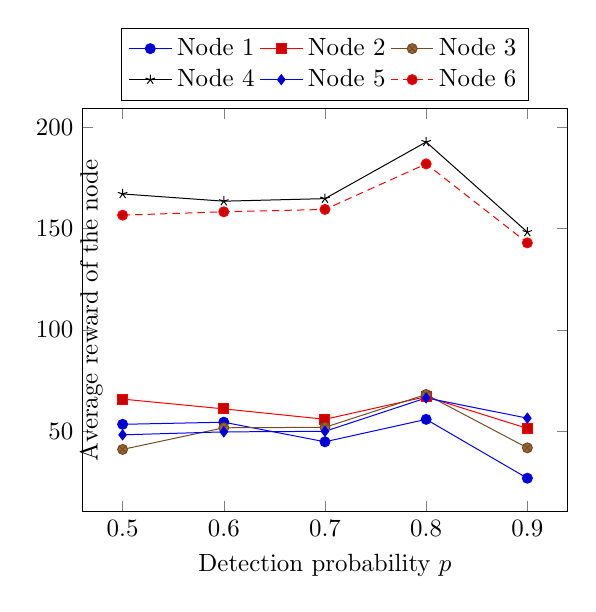
\begin{tikzpicture}[scale=0.9]
\begin{axis}[
  xlabel={Detection probability $p$},
  ylabel={Average reward of the node },
  y label style={at={(0.06,0.5)}},
  xtick={0.5,0.6,0.7,0.8,0.9,1.0},
  legend style={at={(0.5,1.2)},cells={align=right}, anchor=north,legend columns=3},
  grid style=dashed,
]

\addplot+[]
    coordinates {
(0.5,53.3115955435)(0.6,54.3545841648)(0.7,44.6785742262)(0.8,55.7545888625)(0.9,26.6726622755)
};

\addplot+[]
    coordinates {
(0.5,65.7687020142)(0.6,60.9406466924)(0.7,55.8056247195)(0.8,66.9612779492)(0.9,51.2874064555)
};

\addplot+[]
    coordinates {
(0.5,40.908080525)(0.6,51.5966479036)(0.7,51.8294937238)(0.8,68.0588803377)(0.9,41.6899098384)
};

\addplot+[]
    coordinates {
(0.5,167.1425811)(0.6,163.56587834)(0.7,164.826844567)(0.8,192.814744826)(0.9,148.302330965)
};

\addplot+[]
    coordinates {
(0.5,48.1098633801)(0.6,49.569538244)(0.7,49.8423884228)(0.8,66.3485362884)(0.9,56.3535029043)
};

\addplot+[]
    coordinates {
(0.5,156.653749239)(0.6,158.321084535)(0.7,159.485991256)(0.8,181.985919611)(0.9,142.979383044)
};

\legend{Node 1, Node 2, Node 3, Node 4, Node 5, Node 6}
\end{axis}
\end{tikzpicture}
% \label{fig:nodeimp_single}
\end{subfigure}
% \hspace*{\fill}
\begin{subfigure}{.5\textwidth}
\caption{Scenario b)}
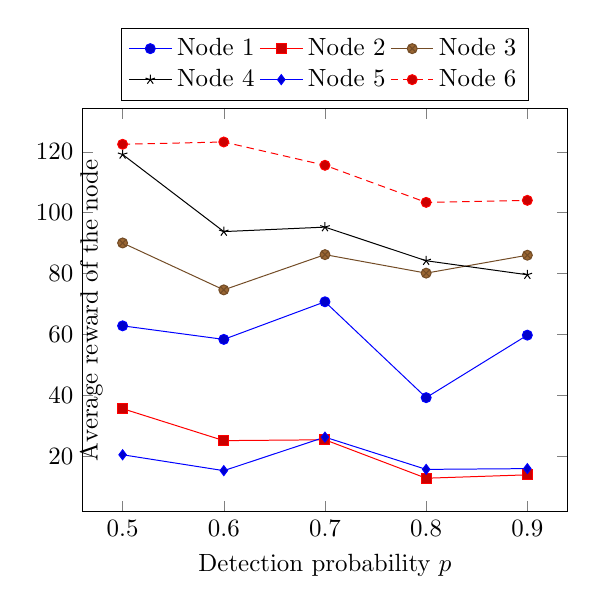
\begin{tikzpicture}[scale=0.9]
\begin{axis}[
  xlabel={Detection probability $p$},
  ylabel={Average reward of the node },
  y label style={at={(0.06,0.5)}},
  xtick={0.5,0.6,0.7,0.8,0.9,1.0},
  legend style={at={(0.5,1.2)},cells={align=right}, anchor=north,legend columns=3},
  grid style=dashed,
]

\addplot+[]
    coordinates {
(0.5,62.8521432343)(0.6,58.3969143024)(0.7,70.7528787794)(0.8,39.262008432)(0.9,59.7930672705)
};

\addplot+[]
    coordinates {
(0.5,35.6477622245)(0.6,25.1466084924)(0.7,25.4245369898)(0.8,12.7966666667)(0.9,13.9088095238)
};

\addplot+[]
    coordinates {
(0.5,90.0722009288)(0.6,74.6625998331)(0.7,86.2388746563)(0.8,80.1605264877)(0.9,86.0444903266)
};

\addplot+[]
    coordinates {
(0.5,119.130037557)(0.6,93.8066520365)(0.7,95.2732464682)(0.8,84.2315618108)(0.9,79.6278821173)
};

\addplot+[]
    coordinates {
(0.5,20.5031617844)(0.6,15.2818516008)(0.7,26.2961789474)(0.8,15.7022412698)(0.9,15.9502350792)
};

\addplot+[]
    coordinates {
(0.5,122.48657341)(0.6,123.23710488)(0.7,115.578393437)(0.8,103.398742076)(0.9,104.070036133)
};

\legend{Node 1, Node 2, Node 3, Node 4, Node 5, Node 6}
\end{axis}
\end{tikzpicture}
% \label{fig:nodeimp_topo1_multiple}
\end{subfigure}
\begin{subfigure}{.5\textwidth}
\caption{Scenario c)}
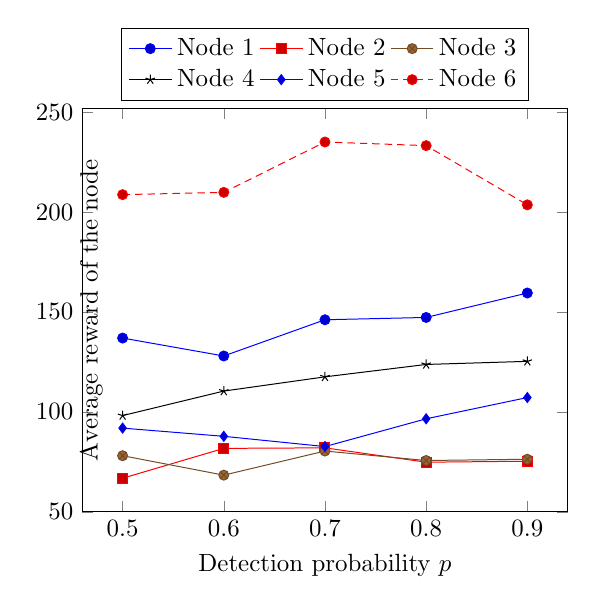
\begin{tikzpicture}[scale=0.9]
\begin{axis}[
  xlabel={Detection probability $p$},
  ylabel={Average reward of the node },
  y label style={at={(0.06,0.5)}},
  xtick={0.5,0.6,0.7,0.8,0.9,1.0},
  legend style={at={(0.5,1.2)},cells={align=right}, anchor=north,legend columns=3},
  grid style=dashed,
]

\addplot+[]
    coordinates {
(0.5,136.927310407)(0.6,127.960388869)(0.7,146.086472254)(0.8,147.235410707)(0.9,159.469537067)
};

\addplot+[]
    coordinates {
(0.5,66.7988560021)(0.6,81.7311837411)(0.7,82.0017291916)(0.8,74.8192160051)(0.9,75.3089759032)
};

\addplot+[]
    coordinates {
(0.5,78.0634438963)(0.6,68.3402801041)(0.7,80.4009699099)(0.8,75.6559526089)(0.9,76.2953944418)
};

\addplot+[]
    coordinates {
(0.5,98.1369317879)(0.6,110.402016785)(0.7,117.520015671)(0.8,123.721254753)(0.9,125.271778646)
};

\addplot+[]
    coordinates {
(0.5,91.8750388819)(0.6,87.764930694)(0.7,82.6400238592)(0.8,96.5305636149)(0.9,107.164379512)
};

\addplot+[]
    coordinates {
(0.5,208.678957661)(0.6,209.815036383)(0.7,235.024736742)(0.8,233.211114765)(0.9,203.573491786)
};

\legend{Node 1, Node 2, Node 3, Node 4, Node 5, Node 6}
\end{axis}
\end{tikzpicture}
\label{fig:nodeimp_topofullmesh_single}
\end{subfigure}
\begin{subfigure}{.5\textwidth}
\caption{Scenario d)}
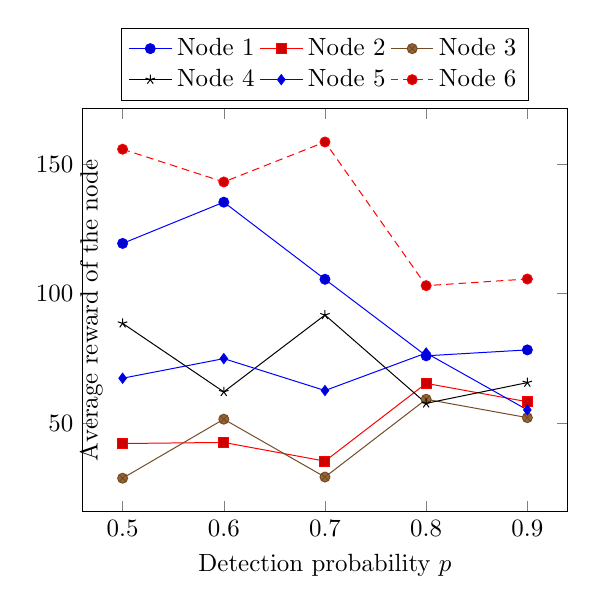
\begin{tikzpicture}[scale=0.9]
\begin{axis}[
  xlabel={Detection probability $p$},
  ylabel={Average reward of the node },
  y label style={at={(0.06,0.5)}},
  xtick={0.5,0.6,0.7,0.8,0.9,1.0},
  legend style={at={(0.5,1.2)},cells={align=right}, anchor=north,legend columns=3},
  grid style=dashed,
]
\addplot+[]
    coordinates {
(0.5,119.371712601)(0.6,135.286667912)(0.7,105.529600824)(0.8,75.9989590936)(0.9,78.2753189412)
};

\addplot+[]
    coordinates {
(0.5,42.1375403255)(0.6,42.565143412)(0.7,35.3397856269)(0.8,65.3575977521)(0.9,58.2605813704)
};

\addplot+[]
    coordinates {
(0.5,28.7468808547)(0.6,51.5357784637)(0.7,29.2058743109)(0.8,59.2143811265)(0.9,52.1289422766)
};

\addplot+[]
    coordinates {
(0.5,88.5226866406)(0.6,62.0702732607)(0.7,91.7445586432)(0.8,57.6471392951)(0.9,65.6462507676)
};

\addplot+[]
    coordinates {
(0.5,67.3444699973)(0.6,74.9142598942)(0.7,62.5913086947)(0.8,77.0770283465)(0.9,55.1241141827)
};

\addplot+[]
    coordinates {
(0.5,155.731553105)(0.6,143.087791722)(0.7,158.519494584)(0.8,103.069877877)(0.9,105.637179687)
};


\legend{Node 1, Node 2, Node 3, Node 4, Node 5, Node 6}
\end{axis}
\end{tikzpicture}
% \label{fig:nodeimp_topofullmesh_multiple}
\end{subfigure}
\begin{subfigure}{.5\textwidth}
\caption{Scenario e)}
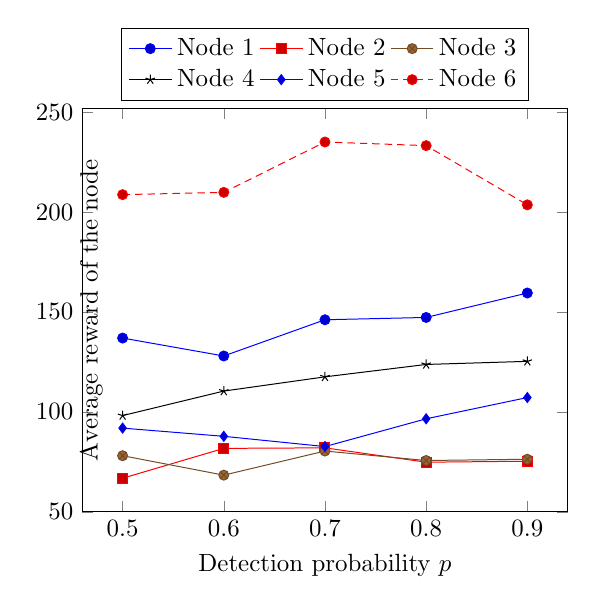
\begin{tikzpicture}[scale=0.9]
\begin{axis}[
  xlabel={Detection probability $p$},
  ylabel={Average reward of the node },
  y label style={at={(0.06,0.5)}},
  xtick={0.5,0.6,0.7,0.8,0.9,1.0},
  legend style={at={(0.5,1.2)},cells={align=right}, anchor=north,legend columns=3},
  grid style=dashed,
]

\addplot+[]
    coordinates {
(0.5,136.927310407)(0.6,127.960388869)(0.7,146.086472254)(0.8,147.235410707)(0.9,159.469537067)
};

\addplot+[]
    coordinates {
(0.5,66.7988560021)(0.6,81.7311837411)(0.7,82.0017291916)(0.8,74.8192160051)(0.9,75.3089759032)
};

\addplot+[]
    coordinates {
(0.5,78.0634438963)(0.6,68.3402801041)(0.7,80.4009699099)(0.8,75.6559526089)(0.9,76.2953944418)
};

\addplot+[]
    coordinates {
(0.5,98.1369317879)(0.6,110.402016785)(0.7,117.520015671)(0.8,123.721254753)(0.9,125.271778646)
};

\addplot+[]
    coordinates {
(0.5,91.8750388819)(0.6,87.764930694)(0.7,82.6400238592)(0.8,96.5305636149)(0.9,107.164379512)
};

\addplot+[]
    coordinates {
(0.5,208.678957661)(0.6,209.815036383)(0.7,235.024736742)(0.8,233.211114765)(0.9,203.573491786)
};

\legend{Node 1, Node 2, Node 3, Node 4, Node 5, Node 6}
\end{axis}
\end{tikzpicture}
% \label{fig:nodeimp_topo2_single}
\end{subfigure}
\begin{subfigure}{0.5\textwidth}
\caption{Scenario f)}
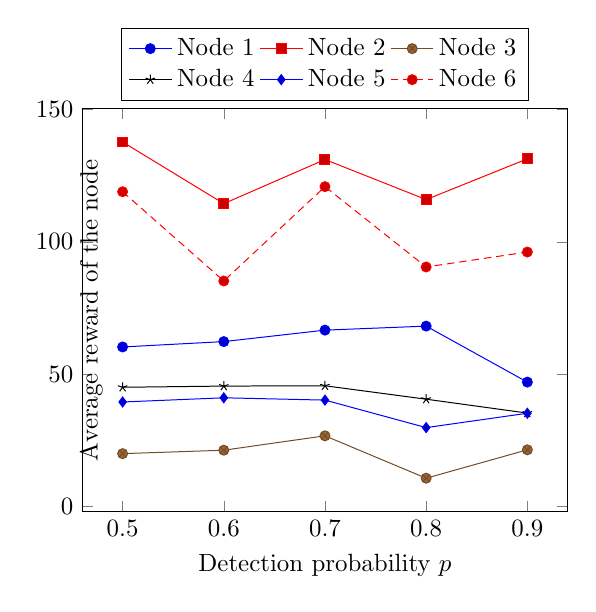
\begin{tikzpicture}[scale=0.9]
\begin{axis}[
  xlabel={Detection probability $p$},
  ylabel={Average reward of the node },
  y label style={at={(0.06,0.5)}},
  xtick={0.5,0.6,0.7,0.8,0.9,1.0},
  legend style={at={(0.5,1.2)},cells={align=right}, anchor=north,legend columns=3},
  grid style=dashed,
]

\addplot+[]
    coordinates {
(0.5,60.2573589594)(0.6,62.2897498389)(0.7,66.6189296773)(0.8,68.1381242941)(0.9,46.9747690794)
};

\addplot+[]
    coordinates {
(0.5,137.718591959)(0.6,114.415855021)(0.7,131.098099496)(0.8,115.956525872)(0.9,131.342366518)
};

\addplot+[]
    coordinates {
(0.5,19.9434781525)(0.6,21.2453007497)(0.7,26.6861654702)(0.8,10.6570889308)(0.9,21.3953375637)
};

\addplot+[]
    coordinates {
(0.5,45.028440798)(0.6,45.476076193)(0.7,45.5952834274)(0.8,40.5190352759)(0.9,35.2739320333)
};

\addplot+[]
    coordinates {
(0.5,39.4612966034)(0.6,41.0516205098)(0.7,40.1801733076)(0.8,29.7830035165)(0.9,35.211062317)
};

\addplot+[]
    coordinates {
(0.5,118.924992552)(0.6,85.1897448279)(0.7,120.841664824)(0.8,90.4846271321)(0.9,96.1337520102)
};

\legend{Node 1, Node 2, Node 3, Node 4, Node 5, Node 6}
\end{axis}
\end{tikzpicture}


% \label{fig:nodeimp_topo2_multiple}
\end{subfigure}
    \caption{Results for single and multiple attackers}
    \label{fig:mdp-results}
\end{figure}
% \clearpage

% }

% \FC{a relire}
\subsection{Experimental results: individual performance}
 We detail the results for each use case, and the performance of each node monitoring the infrastructure.
 Results are shown in Figure~\ref{fig:mdp-results}.
%  \GB{The figure is dense. Subfigures are too close to each other, in particular, the title of one subfigure with the caption of the below subfigure. Also captions for the right column are not centered.}.

\subsubsection*{Balanced topology: Scenarios a) and b)}
Based on the paths taken by the attacks and the ordering of the migration, we categorize the nodes into three categories: source, intermediate and border nodes. Source nodes are the origins of the attacks, intermediate nodes are the first hop from an attack node and border nodes are two hops or more away.
Scenario a) sets node 6 as the source; nodes 4 and 5 as intermediate nodes; and finally nodes 1, 2 and 3 as border nodes.
Scenario b) sets nodes 3 and 6 as sources; nodes 1 and 4 as intermediate nodes; and nodes 2 and 5 as border nodes.
The first observation is that nodes 4 and 6 are the most rewarding nodes.
This is explained as node 6 is the source of most of the attacks, and the exfiltrated data are redirected there. Node 4 is the next hop of attacks directed toward the Virtual Network (nodes 1, 2, and 3).

In both scenarios, the importance of nodes is separated according to our categorization. 
This means that the nodes pertaining to the majority of attack paths are the most rewarding.
This observation is reinforced in scenario b) where nodes 1 and 4 are closer to attack sources while nodes 2 and 5 are further away.

% In scenario a) results are stable from $p=0.6$ where node 6 overcomes node 4 in reward until $p=0.9$. All other nodes remain closely grouped, and no intermediate or border nodes is standing out.
In scenario b) the importance of node 3 increases as the importance of node 6 decreases.
The performance of the monitoring makes it more efficient to monitor the second source of attacks.


\subsubsection*{Full-mesh topology: Scenarios c) and d)}
In these scenarios, the considered topology is full-meshed, which means that each physical node is connected to every other node of the infrastructure. This topology has been chosen to minimize the impact of the routing on the detection path because the attacker is always directly connected to the target node.
Therefore, there are only two categoeries: attack nodes and intermediate nodes.
We make two observations from the results of both scenarios.
The first observation is that this topology is very sensitive to the number of attackers in the infrastructure. In the balanced topology, the nodes have the same ranking whether there is one or two attackers. This result does not hold for a full-meshed topology. In scenario c), the source of attacks globally performs better than intermediate nodes, while in scenario d) both attack and intermediate nodes have more similar rewards.

The second observation is that the detection probability tends to be more impacting in scenario d) than c). This can be explained because detection paths are more diverse with multiple attackers. Indeed, in scenario c) the focus is set on the source of attacks and then determining which nodes are the most attacked.
In scenario d) it becomes more complex to find a monitoring node that covers most attacks, as the detection can only be performed at the source of attacks and at the targeted node.

% Finally, we have examined the different optimal policies for these scenarios, and observed that some corner cases have appeared.
% Overall, the fact that for each attack only the origin of the attack and the target node may contribute to the detection has generated a diverse solution state. Simply put, 

% Each solution is composed of only two nodes. Because of the fullmesh aspect of the topology, it is complex to obtain a solution state 
% Indeed, depending on which node is targeted, there are only two nodes in the solution for the detection of the attack. and the fullmesh aspect of the topology makes it hard for those solution sets to overlap and give a better coverage.

\subsubsection*{Central topology: Scenarios e) and f)}
Using the same categorization as scenarios a) and b), we consider node 6 as a source node, node 2 as an intermediate node and nodes 1, 3, 4 and 5 as border nodes. 
Scenario f) sets nodes 1 and 6 as source nodes, nodes 2 and 4 as intermediate nodes and nodes  3 and 5 as border nodes.

In scenario e), the importance of each node reflects their role. Nodes 3, 4 and 5 do not have much impact in the solution set as they are not on the path of most attacks, while node 1 remains the main target at the beginning of the migration. The attack source, node 6, is still considered important to monitor.

Scenario f) highlights similar results. There are now two attack sources, nodes 1 and 6. Moreover, the geographical distribution of migrated nodes gives more importance to node 2 which becomes even more present on the attack paths, as shown in Table~\ref{tab:mdp-attack-source}. The fact that node 2 acts as a ``bridge" is really highlighted with two attackers.


% Optimal policies also have some corner cases with counter intuitive optimal monitoring nodes but those remain marginal considering the solution space. 

% \FC{Ajout - A relire}
\subsection{Summary}

The analysis of the results outlines several aspects common to each scenario.
The detection rate does not have a significant impact on the importance of nodes, as they remain ranked in the same order, except for scenario d) as we detailed.
% The steadiness in the evolution of each node shows that the performance of the detection is not a major factor in determining which nodes are best suited for the monitoring.
% We formulate some hypotheses in Section~\ref{sec:mdp-discussion}.

Detailed examination of the optimal policy for each budget also shows that the monitoring action is rarely used to redeploy resources elsewhere in the infrastructure.
Instead of unmonitoring nodes, the MDP chooses to do nothing to preserve the global detection probability.
Unmonitoring actions are only chosen when the the node to be unmonitored is not on the path of the next attacks, thus having the same impact as doing nothing. 
This situation happens rarely, when the attacker launches a limited number of attacks on the infrastructure.

% \begin{figure}
    \centering
    \captionsetup[subfigure]{labelformat=empty}
\begin{subfigure}{.5\textwidth}
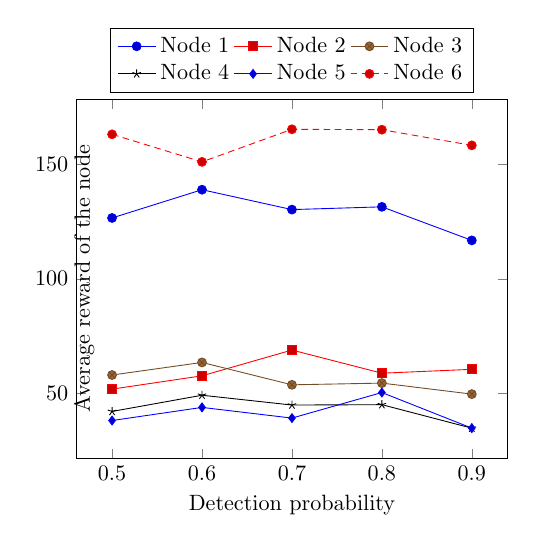
\begin{tikzpicture}[scale=0.8]
\begin{axis}[
  xlabel={Detection probability},
  ylabel={Average reward of the node },
  y label style={at={(0.06,0.5)}},
  xtick={0.5,0.6,0.7,0.8,0.9,1.0},
  legend style={at={(0.5,1.2)},cells={align=right}, anchor=north,legend columns=3},
  grid style=dashed,
]

\addplot+[]
    coordinates {
(0.5,126.469294224)(0.6,138.768688772)(0.7,130.10979383)(0.8,131.308647284)(0.9,116.70873472)
};

\addplot+[]
    coordinates {
(0.5,51.9774584454)(0.6,57.7615872131)(0.7,68.9811633084)(0.8,58.9060250618)(0.9,60.5911805552)
};

\addplot+[]
    coordinates {
(0.5,58.112876005)(0.6,63.5894390224)(0.7,53.8483204974)(0.8,54.5969922461)(0.9,49.8027670671)
};

\addplot+[]
    coordinates {
(0.5,42.2594496478)(0.6,49.3133895991)(0.7,45.0502147208)(0.8,45.20918204)(0.9,34.9808016775)
};

\addplot+[]
    coordinates {
(0.5,38.3055097066)(0.6,44.0188235767)(0.7,39.3680288222)(0.8,50.4912779668)(0.9,34.9978557067)
};

\addplot+[]
    coordinates {
(0.5,162.87848727)(0.6,150.876767477)(0.7,165.06110317)(0.8,164.882126918)(0.9,158.067481047)
};

\legend{Node 1, Node 2, Node 3, Node 4, Node 5, Node 6}
\end{axis}
\end{tikzpicture}

\caption{Scenario c)}
\label{fig:nodeimp_topofullmesh_single}
\end{subfigure}
\begin{subfigure}{.33\textwidth}
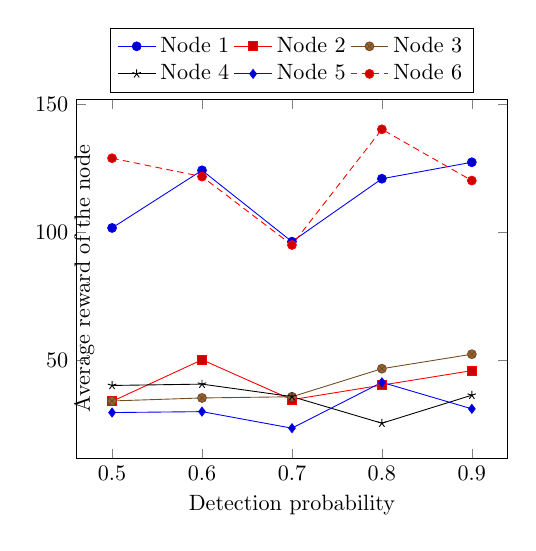
\begin{tikzpicture}[scale=0.8]
\begin{axis}[
  xlabel={Detection probability},
  ylabel={Average reward of the node },
  y label style={at={(0.06,0.5)}},
  xtick={0.5,0.6,0.7,0.8,0.9,1.0},
  legend style={at={(0.5,1.2)},cells={align=right}, anchor=north,legend columns=3},
  grid style=dashed,
]
\addplot+[]
    coordinates {
(0.5,101.616873023)(0.6,124.145242333)(0.7,96.2616914651)(0.8,120.862819291)(0.9,127.305784272)
};

\addplot+[]
    coordinates {
(0.5,33.8037034841)(0.6,50.0693289402)(0.7,34.460597311)(0.8,40.1535742549)(0.9,45.8166364524)
};

\addplot+[]
    coordinates {
(0.5,33.9581528218)(0.6,35.1326808601)(0.7,35.6074089582)(0.8,46.5769811834)(0.9,52.2400544067)
};

\addplot+[]
    coordinates {
(0.5,40.0224063598)(0.6,40.5434953331)(0.7,35.6681036149)(0.8,25.2556265302)(0.9,36.2111392677)
};

\addplot+[]
    coordinates {
(0.5,29.4251886633)(0.6,29.7859232959)(0.7,23.3183642626)(0.8,41.2471235042)(0.9,30.8838558151)
};

\addplot+[]
    coordinates {
(0.5,128.882560148)(0.6,121.704109507)(0.7,94.9489538016)(0.8,140.19719198)(0.9,120.142225907)
};


\legend{Node 1, Node 2, Node 3, Node 4, Node 5, Node 6}
\end{axis}
\end{tikzpicture}

\caption{Scenario d)}
\label{fig:nodeimp_topofullmesh_multiple}
\end{subfigure}
\caption{Results for single and multiple attackers - Scenarios c) and d)}
    \label{fig:mdp-result-fullmesh}
\end{figure}
% \begin{figure}
    \centering
    \captionsetup[subfigure]{labelformat=empty}
\begin{subfigure}{.5\textwidth}
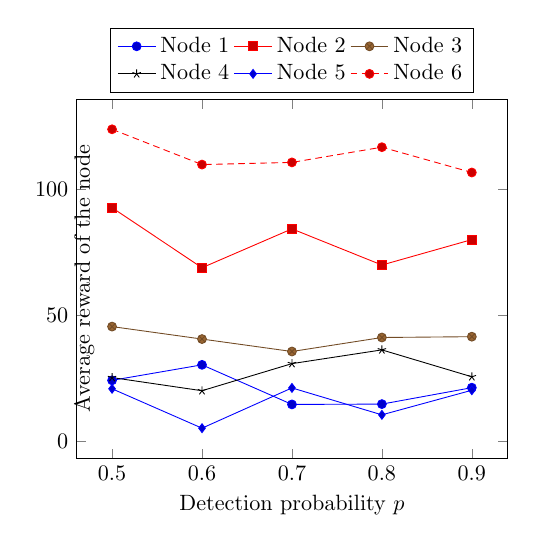
\begin{tikzpicture}[scale=0.8]
\begin{axis}[
  xlabel={Detection probability $p$},
  ylabel={Average reward of the node },
  y label style={at={(0.06,0.5)}},
  xtick={0.5,0.6,0.7,0.8,0.9,1.0},
  legend style={at={(0.5,1.2)},cells={align=right}, anchor=north,legend columns=3},
  grid style=dashed,
]
\addplot+[]
    coordinates {
(0.5,24.2596903238)(0.6,30.4098004181)(0.7,14.7157392372)(0.8,14.8410159329)(0.9,21.3512325325)
};

\addplot+[]
    coordinates {
(0.5,92.6967638225)(0.6,68.892572501)(0.7,84.3050837463)(0.8,69.9668923619)(0.9,80.051680541)
};

\addplot+[]
    coordinates {
(0.5,45.5695982478)(0.6,40.6246377658)(0.7,35.692885081)(0.8,41.2436256503)(0.9,41.5670235599)
};

\addplot+[]
    coordinates {
(0.5,25.3670893308)(0.6,20.1438895136)(0.7,30.888009803)(0.8,36.3312849347)(0.9,25.6728772368)
};

\addplot+[]
    coordinates {
(0.5,20.9174008986)(0.6,5.30161144168)(0.7,21.2602459651)(0.8,10.5837610733)(0.9,20.3331330431)
};

\addplot+[]
    coordinates {
(0.5,123.776293271)(0.6,109.788318837)(0.7,110.653974948)(0.8,116.685625909)(0.9,106.649803871)
};

\legend{Node 1, Node 2, Node 3, Node 4, Node 5, Node 6}
\end{axis}
\end{tikzpicture}

\caption{Scenario e)}
\label{fig:nodeimp_topo2_single}
\end{subfigure}
\begin{subfigure}{.33\textwidth}
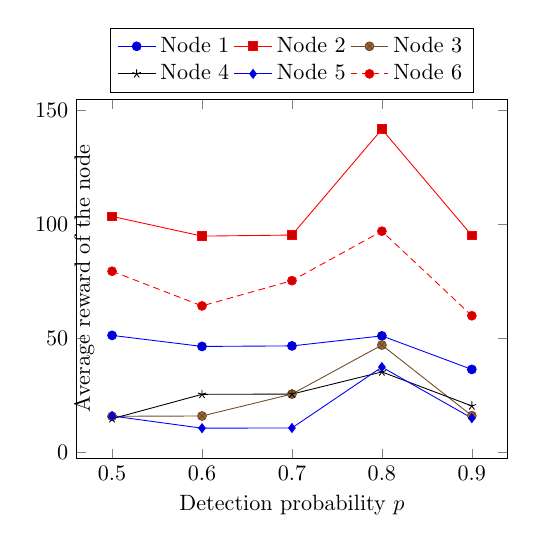
\begin{tikzpicture}[scale=0.8]
\begin{axis}[
  xlabel={Detection probability $p$},
  ylabel={Average reward of the node },
  y label style={at={(0.06,0.5)}},
  xtick={0.5,0.6,0.7,0.8,0.9,1.0},
  legend style={at={(0.5,1.2)},cells={align=right}, anchor=north,legend columns=3},
  grid style=dashed,
]

\addplot+[]
    coordinates {
(0.5,51.2408756424)(0.6,46.3989088055)(0.7,46.629281859)(0.8,51.0165854846)(0.9,36.3262102772)
};

\addplot+[]
    coordinates {
(0.5,103.390154828)(0.6,94.7445634867)(0.7,95.2136135648)(0.8,141.564157095)(0.9,95.0544799628)
};

\addplot+[]
    coordinates {
(0.5,15.7876437463)(0.6,15.9058652472)(0.7,25.5235856726)(0.8,47.0026051031)(0.9,16.0455657836)
};

\addplot+[]
    coordinates {
(0.5,14.6911918445)(0.6,25.4076999562)(0.7,25.5090975344)(0.8,35.2122191081)(0.9,20.3233753667)
};

\addplot+[]
    coordinates {
(0.5,15.9163072098)(0.6,10.573393829)(0.7,10.6704256682)(0.8,37.3424358141)(0.9,14.9838488261)
};

\addplot+[]
    coordinates {
(0.5,79.3520830459)(0.6,64.1507914239)(0.7,75.2190374666)(0.8,96.912552594)(0.9,59.8478399229)
};

\legend{Node 1, Node 2, Node 3, Node 4, Node 5, Node 6}
\end{axis}
\end{tikzpicture}

\caption{Scenario f)}
\label{fig:nodeimp_topo2_multiple}
\end{subfigure}
\caption{Results for single and multiple attackers - Scenarios e) and f)}
    \label{fig:mdp-result-topo2}
\end{figure}



\subsubsection{Determining the optimal monitoring nodes}
When solving a problem using an MDP, the solution is a dynamic proposition to choose actions as the system evolves.
However, from a technical aspect, the defender needs to have the nodes already monitoring the infrastructure before starting the migration process.
It becomes necessary to translate the dynamic answer of the MDP into a static \textit{a priori} deployment.
After determining the individual importance of each node, we propose to determine the optimal set of monitoring nodes.

The main difference is that each node was evaluated based on all the possible budget combinations, whereas what is defined here is a particular answer for a specific budget.
For each budget, the maximum reward is $\frac{b_f}{c_f} \sum\limits_{i \in \textbf{N}}V_i(1-\alpha) $ which corresponds to the corner case where the attacker never launched an attack, and we can evaluate the efficiency of the  monitoring nodes thanks to the associated reward.
Even if a particular monitoring set achieves close to the maximum reward, it is also because this monitoring set is the optimal solution to a specific subset of all possible attacks.
We propose to determine the optimal monitoring state for each budget by weighting the reward they achieve with their occupation of the total solution space.

% We note $S_{\text{abs}}$ the set of absorbing states, 
We note $S^{\text{Mo}}_{\text{abs}}$ the set of absorbing states with a common  monitoring set $Mo$, $\rho(Mo)$ the percentage of presence of set $Mo$ in the solution space and $R(Mo)$ the reward of monitoring set $Mo$.
% \begin{equation}
%     R(Mo) = \sum\limits_{s \in S_{Mo}^{abs}}\rho(Mo^s)R(Mo^s)
% \end{equation}
Then we propose to choose the optimal monitoring set $Mo^*$ with:
\begin{equation}
    Mo^* = \argmax\limits_{\text{Mo}} \left \{\sum\limits_{s \in S^{\text{Mo}}_{\text{abs}}}\rho(Mo^s)R(Mo^s) \right \}
\end{equation}

The optimal monitoring set is determined by choosing the set giving the maximum weighted reward.

% \CK{Les tables sont un peu enormes, reduis un peu leur taille}

% Please add the following required packages to your document preamble:
% \usepackage{multirow}
% \usepackage{graphicx}
\begin{table}[h]
\resizebox{\textwidth}{!}{%
\begin{tabular}{ccccccc}
\multicolumn{3}{c}{\textbf{Scenario a)}}                                                                     &                       & \multicolumn{3}{c}{\textbf{Scenario b)}}                                                                    \\ \cline{1-3} \cline{5-7} 
\multicolumn{1}{|c|}{p}                    & \multicolumn{1}{c|}{($b_f,b_c$)} & \multicolumn{1}{c|}{$Mo^*$}  & \multicolumn{1}{c|}{} & \multicolumn{1}{c|}{p}                    & \multicolumn{1}{c|}{($b_f,b_c$)} & \multicolumn{1}{c|}{$Mo^*$}  \\ \cline{1-3} \cline{5-7} 
\multicolumn{1}{|c|}{\multirow{2}{*}{0.5}} & \multicolumn{1}{c|}{(30,30)}     & \multicolumn{1}{c|}{2,4,6}   & \multicolumn{1}{c|}{} & \multicolumn{1}{c|}{\multirow{2}{*}{0.5}} & \multicolumn{1}{c|}{(30,30)}     & \multicolumn{1}{c|}{2,4,6}   \\ \cline{2-3} \cline{6-7} 
\multicolumn{1}{|c|}{}                     & \multicolumn{1}{c|}{(40,40)}     & \multicolumn{1}{c|}{1,2,4,6} & \multicolumn{1}{c|}{} & \multicolumn{1}{c|}{}                     & \multicolumn{1}{c|}{(40,40)}     & \multicolumn{1}{c|}{1,2,4,6} \\ \cline{1-3} \cline{5-7} 
\multicolumn{1}{|c|}{\multirow{2}{*}{0.7}} & \multicolumn{1}{c|}{(30,30)}     & \multicolumn{1}{c|}{1,4,6}   & \multicolumn{1}{c|}{} & \multicolumn{1}{c|}{\multirow{2}{*}{0.7}} & \multicolumn{1}{c|}{(30,30)}     & \multicolumn{1}{c|}{1,4,6}   \\ \cline{2-3} \cline{6-7} 
\multicolumn{1}{|c|}{}                     & \multicolumn{1}{c|}{(40,40)}     & \multicolumn{1}{c|}{2,3,4,6} & \multicolumn{1}{c|}{} & \multicolumn{1}{c|}{}                     & \multicolumn{1}{c|}{(40,40)}     & \multicolumn{1}{c|}{2,3,4,6} \\ \cline{1-3} \cline{5-7} 
\multicolumn{1}{|c|}{\multirow{2}{*}{0.9}} & \multicolumn{1}{c|}{(30,30)}     & \multicolumn{1}{c|}{4,5,6}   & \multicolumn{1}{c|}{} & \multicolumn{1}{c|}{\multirow{2}{*}{0.9}} & \multicolumn{1}{c|}{(30,30)}     & \multicolumn{1}{c|}{4,5,6}   \\ \cline{2-3} \cline{6-7} 
\multicolumn{1}{|c|}{}                     & \multicolumn{1}{c|}{(40,40)}     & \multicolumn{1}{c|}{1,4,5,6} & \multicolumn{1}{c|}{} & \multicolumn{1}{c|}{}                     & \multicolumn{1}{c|}{(40,40)}     & \multicolumn{1}{c|}{1,4,5,6} \\ \cline{1-3} \cline{5-7} 
                                           &                                  &                              &                       &                                           &                                  &                              \\
\multicolumn{3}{c}{\textbf{Scenario c)}}                                                                     &                       & \multicolumn{3}{c}{\textbf{Scenario d)}}                                                                    \\ \cline{1-3} \cline{5-7} 
\multicolumn{1}{|c|}{p}                    & \multicolumn{1}{c|}{($b_f,b_c$)} & \multicolumn{1}{c|}{$Mo^*$}  & \multicolumn{1}{c|}{} & \multicolumn{1}{c|}{p}                    & \multicolumn{1}{c|}{($b_f,b_c$)} & \multicolumn{1}{c|}{$Mo^*$}  \\ \cline{1-3} \cline{5-7} 
\multicolumn{1}{|c|}{\multirow{2}{*}{0.5}} & \multicolumn{1}{c|}{(30,30)}     & \multicolumn{1}{c|}{1,2,6}   & \multicolumn{1}{c|}{} & \multicolumn{1}{c|}{\multirow{2}{*}{0.5}} & \multicolumn{1}{c|}{(30,30)}     & \multicolumn{1}{c|}{1,3,6}   \\ \cline{2-3} \cline{6-7} 
\multicolumn{1}{|c|}{}                     & \multicolumn{1}{c|}{(40,40)}     & \multicolumn{1}{c|}{1,3}     & \multicolumn{1}{c|}{} & \multicolumn{1}{c|}{}                     & \multicolumn{1}{c|}{(40,40)}     & \multicolumn{1}{c|}{1,2,3,6} \\ \cline{1-3} \cline{5-7} 
\multicolumn{1}{|c|}{\multirow{2}{*}{0.7}} & \multicolumn{1}{c|}{(30,30)}     & \multicolumn{1}{c|}{1,3,6}   & \multicolumn{1}{c|}{} & \multicolumn{1}{c|}{\multirow{2}{*}{0.7}} & \multicolumn{1}{c|}{(30,30)}     & \multicolumn{1}{c|}{1,2,6}   \\ \cline{2-3} \cline{6-7} 
\multicolumn{1}{|c|}{}                     & \multicolumn{1}{c|}{(40,40)}     & \multicolumn{1}{c|}{1,2,3,6} & \multicolumn{1}{c|}{} & \multicolumn{1}{c|}{}                     & \multicolumn{1}{c|}{(40,40)}     & \multicolumn{1}{c|}{1,2,5,6} \\ \cline{1-3} \cline{5-7} 
\multicolumn{1}{|c|}{\multirow{2}{*}{0.9}} & \multicolumn{1}{c|}{(30,30)}     & \multicolumn{1}{c|}{1,3,6}   & \multicolumn{1}{c|}{} & \multicolumn{1}{c|}{\multirow{2}{*}{0.9}} & \multicolumn{1}{c|}{(30,30)}     & \multicolumn{1}{c|}{1,2,6}   \\ \cline{2-3} \cline{6-7} 
\multicolumn{1}{|c|}{}                     & \multicolumn{1}{c|}{(40,40)}     & \multicolumn{1}{c|}{1,2,3,6} & \multicolumn{1}{c|}{} & \multicolumn{1}{c|}{}                     & \multicolumn{1}{c|}{(40,40)}     & \multicolumn{1}{c|}{1,2,3,6} \\ \cline{1-3} \cline{5-7} 
                                           &                                  &                              &                       &                                           &                                  &                              \\
\multicolumn{3}{c}{\textbf{Scenario e)}}                                                                     &                       & \multicolumn{3}{c}{\textbf{Scenario f)}}                                                                    \\ \cline{1-3} \cline{5-7} 
\multicolumn{1}{|c|}{p}                    & \multicolumn{1}{c|}{($b_f,b_c$)} & \multicolumn{1}{c|}{$Mo^*$}  & \multicolumn{1}{c|}{} & \multicolumn{1}{c|}{p}                    & \multicolumn{1}{c|}{($b_f,b_c$)} & \multicolumn{1}{c|}{$Mo^*$}  \\ \cline{1-3} \cline{5-7} 
\multicolumn{1}{|c|}{\multirow{2}{*}{0.5}} & \multicolumn{1}{c|}{(30,30)}     & \multicolumn{1}{c|}{2,3,6}   & \multicolumn{1}{c|}{} & \multicolumn{1}{c|}{\multirow{2}{*}{0.5}} & \multicolumn{1}{c|}{(30,30)}     & \multicolumn{1}{c|}{1,2,6}   \\ \cline{2-3} \cline{6-7} 
\multicolumn{1}{|c|}{}                     & \multicolumn{1}{c|}{(40,40)}     & \multicolumn{1}{c|}{1,2,3,6} & \multicolumn{1}{c|}{} & \multicolumn{1}{c|}{}                     & \multicolumn{1}{c|}{(40,40)}     & \multicolumn{1}{c|}{1,2,3,6} \\ \cline{1-3} \cline{5-7} 
\multicolumn{1}{|c|}{\multirow{2}{*}{0.7}} & \multicolumn{1}{c|}{(30,30)}     & \multicolumn{1}{c|}{2,3,6}   & \multicolumn{1}{c|}{} & \multicolumn{1}{c|}{\multirow{2}{*}{0.7}} & \multicolumn{1}{c|}{(30,30)}     & \multicolumn{1}{c|}{1,2,6}   \\ \cline{2-3} \cline{6-7} 
\multicolumn{1}{|c|}{}                     & \multicolumn{1}{c|}{(40,40)}     & \multicolumn{1}{c|}{2,6}     & \multicolumn{1}{c|}{} & \multicolumn{1}{c|}{}                     & \multicolumn{1}{c|}{(40,40)}     & \multicolumn{1}{c|}{1,2,3,6} \\ \cline{1-3} \cline{5-7} 
\multicolumn{1}{|c|}{\multirow{2}{*}{0.9}} & \multicolumn{1}{c|}{(30,30)}     & \multicolumn{1}{c|}{2,3,6}   & \multicolumn{1}{c|}{} & \multicolumn{1}{c|}{\multirow{2}{*}{0.9}} & \multicolumn{1}{c|}{(30,30)}     & \multicolumn{1}{c|}{1,2,6}   \\ \cline{2-3} \cline{6-7} 
\multicolumn{1}{|c|}{}                     & \multicolumn{1}{c|}{(40,40)}     & \multicolumn{1}{c|}{2,3,5,6} & \multicolumn{1}{c|}{} & \multicolumn{1}{c|}{}                     & \multicolumn{1}{c|}{(40,40)}     & \multicolumn{1}{c|}{1,2,4,6} \\ \cline{1-3} \cline{5-7} 
\end{tabular}%
}
\caption{Optimal monitoring sets of the use cases}
\label{tab:mdp-usecase-optiset}
\end{table}
% \FC{a relire}

\subsection{Experimental results: Monitoring sets}

We describe the optimal monitoring sets for each use case.
Results for all scenarios are summarized in Table~\ref{tab:mdp-usecase-optiset}. 

\subsubsection*{Balanced topology: Scenarios a) and b)}
We note that node 6 is always chosen in the monitoring, as it is the main source of attacks.
Node 4 also always appears as a good candidate for a fourth node if it is not already chosen third.
In both scenarios, we observe that third and fourth nodes rarely coincide between (30, 30) and (40, 40) budgets.
In scenario a), for a (40,40) budget at $p=0.7$,  nodes 2 and 3 are selected instead of reusing the node 1 that was selected for the (30,30) budget.
This suggests that combining two nodes increases their individual performance.
In scenario b) at $p=0.5$, we obtain a similar result where nodes 3 and 4 are considered over node 2.

% We suppose this is because node 1 is surrounded by nodes 2 and 3 in the topology.
% This is explained because other budgets impact the individual importance of each node.

\subsubsection*{Full-mesh topology: Scenarios c) and d)}
One notable result is in scenario c) for $p=0.5,  (b_f,b_c) = (40,40)$ and in scenario d) for $p=0.7,  (b_f,b_c) = (40,40)$, where the optimal monitoring set is \{1,2,5,6\} which does not include node 3 like other budgets.  The explanation comes from the fact that it takes less time to establish the path between the victim's network and the extraction point because of the full-mesh topology. There are only two nodes capable of detecting an attack every time it is started, thus the monitoring of extra nodes does not contribute to a better reward.

We conclude that our results confirm the intuition that a low detection probability ($p=0.5$) coupled to a full-mesh topology may not be the ideal conditions to improve the security of the migration process. 


\subsubsection*{Central topology: Scenarios e) and f)}
Both scenarios exhibit similar results, where nodes 2 and 6 are consistently picked every time.
Indeed, node 6 is the source of attacks, and the MDP also selects node 2 because it is on the path of most attacks as a valuable node.
In scenario e) node 3 is often picked first over node 1, in opposition to scenario f).
This choice is due to the second attack source becoming more valuable in scenario f).

\subsection{Summary}
We have confirmed in every scenario the intuition that the attack source must be part of the monitoring set. Results also show that the second attacker should be monitored.
In some cases, it seems that combining the monitoring of two nodes increases their individual performance (\eg Scenario a) at $p=0.9$, node 5 for budget (30,30) and nodes 2 and 3 for budget (40,40) ).
% Overall, the model outlines which nodes take part in m
% \FC{Verifier p=0.7 scenario e)}

% The other part of the counter intuitive result (not shown in Table~\ref{tab:mdp-usecase-optiset}) is due to removing node 6, the source of attacks from the monitoring. It is worth noting that this particular case represents a negligible portion of the solution space, and most of the counter intuitive results are due to the previous explanation. Considering that node 6 is removed at a point where the consequences of attacks will be minimal, it was deemed equivalent to the ``do nothing" action by the MDP. \CK{Je trouve ce paragraphe (a partir de "The other part of...") pas clair du tout et je ne pense pas qu'il apporte grand chose, je suggere de le supprimer}




\subsubsection{Discussion}
During the evaluation of our model, we have produced several results that shed light on several aspects of our modeling choices.

First of all, the use of budgets as part of the MDP state is a root cause for the complexity in generating the MDP states. Indeed, these budgets act as a sort of "identifiers`` that make the number of states grow exponentially compared to the available budgets.

The second aspect is the use of the financial budget to describe the duration of the migration. The attacker keeps compromising nodes while there can be transitions toward another state. This makes the financial budget behave more like the time period defined to study the migration and its security. This also questions the meaning of the performance impact budget. It appears that the available computational power defines the solution space, the number of different monitoring sets that can exist \etc. 
It can be interesting to explore different budget formats to improve the model.

In the literature the rewards concept does not always account for both current and next state, and sometimes one of the two states is ignored, because the transition probability account for it. We used the MDPToolbox~\cite{Chades2014} to determine the optimal policy  of the MDP, and it considers the reward using the current state only and not the one the system will transition to. We postulate that this simplification does not impact the model very much because the system will always transition toward an absorbing state.
The matter can be worth investigating in case of major changes in the model.

The use cases we proposed did not distinguish virtual networks between one-to-one mapping and one to many-to-many mapping. While arbitrary topologies are an important feature of a virtualization service, in our case we can easily alleviate this issue because physical nodes embedding one single node are part of the virtual topology and thus part of the migration, whether they are made visible to the end user or not.


\subsubsection{Conclusion}
\label{sec:mdp-conclusion}
In this section, we investigated the Resource Allocation problem in a security context. Our objective was to determine which nodes of the infrastructure should be performing monitoring tasks to detect attacks against the migration process.
we proposed a Markovian Decision Process to represent how an infrastructure provider can answer to this RA problem and what are the optimal choices.
We introduced the attacker in the definition of the model, which is a novel approach from a security perspective. MDPs often are modeling only one agent to interact with the system, but the inclusion of an actor of a different nature is rarely considered\GB{so it is not novel, since already proposed.}.
We also provided an experimental prototype for the MDP generation, solving and results analysis  (\url{https://github.com/FabienCharmet/MDPRA}).
Results show that we can determine which nodes provide the best security with regard to current attacks, as well as how the dynamic aspect of the optimal policy can be translated into an \textit{a priori} deployment of the monitoring resources on the nodes.
When the attacker can launch attacks from several sources, the impact of the nodes on the monitoring is much more differentiated and gives a better understanding of their role in the infrastructure.
We also run the simulations on several network topologies to evaluate the impact of the attack routing on the optimal solution. Results show that a full-mesh topology is more complex to defend because of the multitude of attack paths.
% Markov Decision Processes are rarely used for a resource allocation problem in a security context.
We advocate that the flexibility of the formalism can be leveraged to dynamically recompute the destination substrate while the migration is ongoing.
Instead of deciding where to deploy the monitoring, the migration process would use the MDP to predict the target of the next attack and should recompute the embedding of the VN if the next virtual node will be embedded on a compromised physical node. The approach would give additional flexibility to the VNE algorithm and make it more secure\GB{this becomes a Reinforcement Learning approach, right?}.


\subsection{Experimental Results}

\section{Conclusion}
\FC{Leveraging security techniques to determine a better substrate for the migration during an attack }
\FC{Check reference architecture -> security component ideas}


\bibliography{references}{}
\bibliographystyle{ieeetr}

\end{document}
